%% Преамбула TeX-файла

% 1. Стиль и язык
\documentclass[utf8x, times, 14pt]{G7-32} % Стиль (по умолчанию будет 14pt)
\bibliographystyle{gost780u}

% Остальные стандартные настройки убраны в preamble.inc.tex.
\sloppy

% Настройки стиля ГОСТ 7-32
% Для начала определяем, хотим мы или нет, чтобы рисунки и таблицы нумеровались в пределах раздела, или нам нужна сквозная нумерация.
\EqInChapter % формулы будут нумероваться в пределах раздела
\TableInChapter % таблицы будут нумероваться в пределах раздела
\PicInChapter % рисунки будут нумероваться в пределах раздела

% Добавляем гипертекстовое оглавление в PDF
\usepackage[
bookmarks=true, colorlinks=true, unicode=true,
urlcolor=black,linkcolor=black, anchorcolor=black,
citecolor=black, menucolor=black, filecolor=black,
]{hyperref}

\AfterHyperrefFix

\usepackage{microtype}% полезный пакет для микротипографии, увы под xelatex мало чего умеет, но под pdflatex хорошо улучшает читаемость

% Тире могут быть невидимы в Adobe Reader
\ifInvisibleDashes
\MakeDashesBold
\fi


\usepackage{graphicx}   % Пакет для включения рисунков

% С такими оно полями оно работает по-умолчанию:
% \RequirePackage[left=20mm,right=10mm,top=20mm,bottom=20mm,headsep=0pt,includefoot]{geometry}
% Если вас тошнит от поля в 10мм --- увеличивайте до 20-ти, ну и про переплёт не забывайте:
\geometry{right=20mm}
\geometry{left=30mm}
\geometry{bottom=20mm}
\geometry{ignorefoot}% считать от нижней границы текста

\usepackage{rotating}

% доп. позиционирование таблиц
\usepackage{float}

% таблицы с автоматическим определением ширины
\usepackage{tabularx}

% для ультра лютой большой таблицы
\usepackage{xltabular}

% Пакет Tikz
\usepackage{tikz}
\usetikzlibrary{arrows,positioning,shadows}

% Произвольная нумерация списков.
\usepackage{enumerate}

% ячейки в несколько строчек
\usepackage{multirow}

% itemize внутри tabular
\usepackage{paralist,array}
\newcolumntype{Y}{>{\centering\arraybackslash}X}

%\setlength{\parskip}{1ex plus0.5ex minus0.5ex} % разрыв между абзацами
\setlength{\parskip}{1ex} % разрыв между абзацами
\setlength{\intextsep}{4pt}
\setlength{\abovecaptionskip}{4pt}
\setlength{\floatsep}{5pt plus 1.0pt minus 1.0pt}
\usepackage{blindtext}

% Центрирование подписей к плавающим окружениям
%\usepackage[justification=centering]{caption}

\usepackage{newfloat}
\DeclareFloatingEnvironment[
placement={!ht},
name=Equation
]{eqndescNoIndent}
\edef\fixEqndesc{\noexpand\setlength{\noexpand\parindent}{\the\parindent}\noexpand\setlength{\noexpand\parskip}{\the\parskip}}
\newenvironment{eqndesc}[1][!ht]{%
    \begin{eqndescNoIndent}[#1]%
\fixEqndesc%
}
{\end{eqndescNoIndent}}

% Настройки листингов.
\ifPDFTeX
% 8 Листинги

\usepackage{listings}

% Значения по умолчанию
\lstset{
  basicstyle= \footnotesize,
  breakatwhitespace=true,% разрыв строк только на whitespacce
  breaklines=true,       % переносить длинные строки
%   captionpos=b,          % подписи снизу -- вроде не надо
  inputencoding=koi8-r,
  numbers=left,          % нумерация слева
  numberstyle=\footnotesize,
  showspaces=false,      % показывать пробелы подчеркиваниями -- идиотизм 70-х годов
  showstringspaces=false,
  showtabs=false,        % и табы тоже
  stepnumber=1,
  tabsize=4,              % кому нужны табы по 8 символов?
  frame=single
}

% Стиль для псевдокода: строчки обычно короткие, поэтому размер шрифта побольше
\lstdefinestyle{pseudocode}{
  basicstyle=\small,
  keywordstyle=\color{black}\bfseries\underbar,
  language=Pseudocode,
  numberstyle=\footnotesize,
  commentstyle=\footnotesize\it
}

% Стиль для обычного кода: маленький шрифт
\lstdefinestyle{realcode}{
  basicstyle=\scriptsize,
  numberstyle=\footnotesize
}

% Стиль для коротких кусков обычного кода: средний шрифт
\lstdefinestyle{simplecode}{
  basicstyle=\footnotesize,
  numberstyle=\footnotesize
}

% Стиль для BNF
\lstdefinestyle{grammar}{
  basicstyle=\footnotesize,
  numberstyle=\footnotesize,
  stringstyle=\bfseries\ttfamily,
  language=BNF
}

% Определим свой язык для написания псевдокодов на основе Python
\lstdefinelanguage[]{Pseudocode}[]{Python}{
  morekeywords={each,empty,wait,do},% ключевые слова добавлять сюда
  morecomment=[s]{\{}{\}},% комменты {а-ля Pascal} смотрятся нагляднее
  literate=% а сюда добавлять операторы, которые хотите отображать как мат. символы
    {->}{\ensuremath{$\rightarrow$}~}2%
    {<-}{\ensuremath{$\leftarrow$}~}2%
    {:=}{\ensuremath{$\leftarrow$}~}2%
    {<--}{\ensuremath{$\Longleftarrow$}~}2%
}[keywords,comments]

% Свой язык для задания грамматик в BNF
\lstdefinelanguage[]{BNF}[]{}{
  morekeywords={},
  morecomment=[s]{@}{@},
  morestring=[b]",%
  literate=%
    {->}{\ensuremath{$\rightarrow$}~}2%
    {*}{\ensuremath{$^*$}~}2%
    {+}{\ensuremath{$^+$}~}2%
    {|}{\ensuremath{$|$}~}2%
}[keywords,comments,strings]

% Подписи к листингам на русском языке.
\renewcommand\lstlistingname{Листинг}
\renewcommand\lstlistlistingname{Листинги}

\else
\usepackage{local-minted}
\fi

% Полезные макросы листингов.
%% Любимые команды
\newcommand{\Code}[1]{\textbf{#1}}

%\usepackage{unicode-math}
\DeclareMathOperator*{\Dap}{Δ P_c}

% Стиль титульного листа и заголовки
%\include{00-title}


\begin{document}

\frontmatter % выключает нумерацию ВСЕГО; здесь начинаются ненумерованные главы: реферат, введение, глоссарий, сокращения и прочее.

\maketitle %создает титульную страницу


%\begin{executors}
%\personalSignature{Первый исполнитель}{ФИО}
%
%\personalSignature{Второй исполнитель}{ФИО}
%\end{executors}


%\listoffigures                         % Список рисунков

%\listoftables                          % Список таблиц

%\NormRefs % Нормативные ссылки 
% Команды \breakingbeforechapters и \nonbreakingbeforechapters
% управляют разрывом страницы перед главами.
% По-умолчанию страница разрывается.

% \nobreakingbeforechapters
% \breakingbeforechapters

%% Также можно использовать \Referat, как в оригинале
\begin{abstract}

   Для электрической сети, схема которой показана на *, на основании исходных данных по узлам и ветвям, приведенных в табл. * и *:
   
   \begin{enumerate}[1.]
   	\item Составить схему замещения сети и определить ее параметры
   	\item Выполнить расчеты потокораспределения и напряжений в узлах сети в нормальном режиме наибольших нагрузок.
   	\item Выполнить расчеты потокораспределения и напряжений в узлах сети в нормальном режиме наименьших нагрузок.
   	\item Выполнить расчеты потокораспределения и напряжений в узлах сети в послеаварийном
   	режиме (отключение одной цепи линии).
   	\item Оценить достаточность регулировочных диапазонов устройств РПН трансформаторов на
   	подстанции.
   	\item Рассчитать потери активной мощности и годовые потери электроэнергии в сети.
   \end{enumerate}

\end{abstract}

%%% Local Variables: 
%%% mode: latex
%%% TeX-master: "rpz"
%%% End: 


\tableofcontents

%\printnomenclature % Автоматический список сокращений



\include{00-intro}

\mainmatter % это включает нумерацию глав и секций в документе ниже

\chapter{Характеристика исходных данных курсового проекта}
\label{cha:ish_dannie}

\newcolumntype{Z}{>{\centering\arraybackslash}X}

\section{Исходные данные для проектирования}

Электрическая сеть сооружается в Костромской области на железобетонных опорах.

\begin{figure}[h]
	\centering
	\includegraphics[width=0.7\textwidth]{inc/svg/scheme}
	\caption{Схема расположения пунктов}
	\label{fig:scheme}
\end{figure}

Питание района электроэнергией будет осуществляться от шин 220 кВ подстанции "К" работающей в составе электроэнергетической системы. Источник питания в режиме наибольших нагрузок обеспечивает полную выдачу необходимой для потребителей активной мощности, а также 87 Мвар реактивной мощности. На шинах источника питания района в режиме наибольших нагрузок обеспечивается напряжение, равно 110 \%, а в режиме наименьших нагрузок 100 \% от номинального.

Для всех пунктов наименьшая нагрузка принимается 37 \% от наибольшей; число часов использования наибольших нагрузок составляет \(4350\; \frac{\textup{ч}}{\textup{год}}\).

Вторичное напряжение на всех сооружаемых подстанциях 10 кВ.

\section{Исходные данные по климатическим условиям и нагрузкам в пунктах потребления}

Среднеянварская температура: \(-11,8\; ^oC\)

Среднегодовая температура: \(2,7\; ^oC\)

Среднеиюльская температура: \(17,6\; ^oC\)

Ветровой район: I

Район по гололёду: I

Определим коэффициент реактивной мощности нагрузки \(\tg \, \varphi_\textup{нб1}\), потребляемую реактивную мощность \(Q_\textup{нб1}\) и полную мощность \(S_\textup{нб1}\) для пункта 1:
\[\tg \, \varphi_\textup{нб1} = \tg(\arccos(\cos\, \varphi_\textup{нб1})) = \tg(\arccos(0,92)) = 0,426\]
\[Q_\textup{нб1} = P_\textup{нб1} \cdot \tg\, \varphi_\textup{нб1} = 70 \cdot 0,426 = 29,8\; \textup{Мвар}\]
\[S_\textup{нб1} = \sqrt{P_\textup{нб1}^2 + Q_\textup{нб1}^2} = \sqrt{70^2 + 29,8^2} = 76,1\; \textup{МВА}\]

Сведем результаты расчета для всех пяти пунктов в таблицу \ref{tab:nagruzki}


\begin{table}[ht]
	\small
	\caption{Исходные данные по нагрузкам в пунктах потребления}
	\begin{tabularx}{\textwidth}{|X|Z|Z|Z|Z|Z|Z|}
		\hline
		Пункт                             & 1     & 2     & 3     & 4     & 5     & $\Sigma$ \\ \hline
		$P_\textup{нб},\; \textup{МВт}$   & 70    & 70    & 30    & 40    & 35    & 245 \\ \hline
		$\cos\, \varphi_\textup{нб}$      & 0,92  & 0,92  & 0,91  & 0,89  & 0,91  & "--- \\ \hline
		$\tg\, \varphi_\textup{нб}$       & 0,426 & 0,426 & 0,456 & 0,512 & 0,456 & "--- \\ \hline
		$Q_\textup{нб}, \; \textup{Мвар}$ & 29,8  & 29,8  & 13,7  & 20,5  & 16,0  & 109,8 \\ \hline
		$S_\textup{нб}, \; \textup{МВА}$  & 76,1  & 76,1  & 33,0  & 44,9  & 38,5  & 268,6 \\ \hline
	\end{tabularx}
	\label{tab:nagruzki}
\end{table}

\section{Определение длин пролётов}
Определим длины воздушных линий между пунктами и сведем результаты в таблицу \ref{tab:dlina}
\begin{table}[H]
	\small
	\caption{Расстояние между пунктами $l_{ij(m)}$, в клеточках}
	\begin{tabularx}{\textwidth}{|X|Z|Z|Z|Z|Z|Z|}
		\hline
		Пункты & К    & 1     & 2     & 3     & 4     & 5     \\ \hline
		К      & "--- & 3,606 & 4,243 & "---  & "---  & "---  \\ \hline
		1      &      & "---  & 5     & 4,243 & 5,385 & "---  \\ \hline
		2      &      &       & "---  & 3,606 & "---  & "---  \\ \hline
		3      &      &       &       & "---  & 2,236 & 4     \\ \hline
		4      &      &       &       &       & "---  & 2,236 \\ \hline
		5      &      &       &       &       &       & "---  \\ \hline
	\end{tabularx}
	\label{tab:dlina}
\end{table}

Протяженность намечаемых воздушных линий при отсутствии точных данных рекомендуется принимать с учетом удлинения трасс линий (по сравнению с наикратчайшим расстоянием между пунктами по воздушной прямой) за счет их непрямолинейности:
\begin{eqndesc}[H]
	\begin{equation}
		L_{ij} = l_{ij} k_\textup{удл},
	\end{equation}

	где $L_{ij}$ "--- длина воздушной линии между пунктами i и j, км; \\
	$l_{ij}$ "--- наикратчайшее расстояние между пунктами i и j по воздушной прямой, км; \\
	$k_\textup{удл}$ "--- коэффициент удлинения трассы воздушной линии (табл. \ref{tab:k_udl}).
\end{eqndesc}

\begin{table}[H]
	\small
	\caption{Коэффициенты удлинения трассы воздушных линий ($k_\textup{удл}$)}
	\begin{tabularx}{\textwidth}{|X|Z|Z|Z|Z|Z|Z|Z|}
		\hline
		Регион           & Центр & Северо-Запад & Северный Кавказ & Средняя Волга & Урал & Сибирь & Восток \\ \hline
		$k_\textup{удл}$ & 1,16  & 1,20         & 1,26            & 1,16          & 1,16 & 1,20   & 1,20   \\ \hline
	\end{tabularx}
	\label{tab:k_udl}
\end{table}
Для Костромы (Центр) $k_\textup{удл} = 1,16$

Наикратчайшее расстояние между пунктами i и j по воздушной прямой пересчитаем в масштабе по формуле:
\[l_{ij} = l_{ij(m)} \cdot m\]

Соотношение масштаба m равно 1:10. Тогда пересчитаем длины воздушных линий между пунктами и сведем результаты в таблицу \ref{tab:dlina_pereschet}
\begin{table}[H]
	\small
	\caption{Расстояние между пунктами $L_{ij}$, км}
	\begin{tabularx}{\textwidth}{|X|Z|Z|Z|Z|Z|Z|}
		\hline
		Пункты & К    & 1    & 2    & 3    & 4    & 5    \\ \hline
		К      & "--- & 41,8 & 49,2 & "--- & "--- & "--- \\ \hline
		1      &      & "--- & 58,0 & 49,2 & 62,5 & "--- \\ \hline
		2      &      &      & "--- & 41,8 & "--- & "--- \\ \hline
		3      &      &      &      & "--- & 25,9 & 46,4 \\ \hline
		4      &      &      &      &      & "--- & 25,9 \\ \hline
		5      &      &      &      &      &      & "--- \\ \hline
	\end{tabularx}
	\label{tab:dlina_pereschet}
\end{table}

\section{Оценка суммарной активной мощности, потребляемой в проектируемой сети, и значения коэффициентов реактивной мощности}
При определении одновременно потребляемой активной мощности (с учетом наибольших нагрузок пунктов потребления и потерь активной мощности в элементах электрической сети) следует учитывать несовпадения по времени суток наибольших нагрузок (НБ) отдельных потребителей. При перспективном проектировании, когда точные графики нагрузок потребителей неизвестны, используют среднестатистические значения  коэффициентов одновременности нагрузок. Таким образом, суммарая активная мощность, потребляемая в проектируемой сети, составляет:
\begin{eqndesc}[H]
	\begin{equation}
		P_{\textup{треб}\Sigma} = k_\textup{однP} \cdot \sum^n_{i=1} P_{\textup{нб}i} + \Dap_* \cdot \sum^n_{i=1} P_{\textup{нб}i},
		\label{eqn:p_treb_sum}
	\end{equation}
	где $P_{\textup{нб}i}$ "--- наибольшая активная нагрузка \textit{i}-го пункта потребления; \\
	\textit{n} "--- число пунктов потребления электроэнергии; \\
	$k_\textup{однP}$ "--- коэффициент одновременности наибольших активных нагрузок подстанций; \\
	${\displaystyle \Dap_*}$ "--- суммарные потери активной мощности в элементах сети в долях от суммарной нагрузки подстанций.
\end{eqndesc}

При четырех и более пунктах среднестатистическое значение $k_{\textup{одн}}$ на шинах 220 кВ источника питания (ИП) составляет 0,95-0,96 \%

Характерные значения суммарных потерь активной мощности в электрических сетях 110-220 кВ оставляют (4-5)\%. Тогда по формуле \eqref{eqn:p_treb_sum}:

\[P_{\textup{треб}\Sigma} = 0,95 \cdot (70 + 70 + 30 + 40 + 50) + 0,05 \cdot (70 + 70 + 30 + 40 + 50) = 260\; \textup{МВт}\]

В соответствии с Приказом Министерства промышленности и энергетики от 22.02.2007 N 49 предельное значение коэффициента реактивной мощности на шинах 10 кВ понижающий ПС: \(\tg\, \varphi_\textup{пред} = 0,4\)

Из таблицы \ref{tab:nagruzki} видно, что во всех пяти пунктах потребления значение коэффициента реактивной мощности больше предельного значения \(\tg\, \varphi_\textup{пред} = 0,4\), следовательно на этих ПС нужно установить компенсирующие устройства (КУ). Мощность требуемых КУ рассчитывается по формуле:

\begin{equation}
	Q_{\textup{КУ}i} = P_{\textup{нб}i} (\tg\, \varphi_i - \tg\, \varphi_\textup{пред})
	\label{eqn:pow_comp_device}
\end{equation}

В качестве примера рассчитаем мощность требуемых КУ для ПС1 по формуле \eqref{eqn:pow_comp_device}:
\[
Q_\textup{КУ1} = 70(0,426 - 0,4) = 1,82\; \textup{Мвар}
\]

Для остальных пунктов расчет выполняется аналогично. Результат запишем в табл. \ref{tab:q_ku}

\begin{table}[ht]
	\small
	\caption{Исходные данные по нагрузкам в пунктах потребления}
	\begin{tabularx}{\textwidth}{|l|Z|Z|Z|Z|Z|Z|}
		\hline
		Пункт                             & 1    & 2    & 3    & 4    & 5    & $\Sigma$ \\ \hline
		$Q_\textup{КУ},\; \textup{МВар}$  & 1,82 & 1,82 & 1,68 & 4,48 & 1,96 & 118     \\ \hline
		$Q_\textup{БСК},\; \textup{МВар}$ & 2,4  & 2,4  & 2,4  & 4,8  & 2,4  & 14,4     \\ \hline
		$Q_\textup{нб},\; \textup{МВар}$  & 27,4 & 27,4 & 11,3 & 15,7 & 13,6 & 95,4     \\ \hline
	\end{tabularx}
	\label{tab:q_ku}
\end{table}

Основным типом компенсирующих устройств условно устанавливаемых на шинах 10 кВ понижающих ПС являются батареи статических конденсаторов (БСК). Устанавливаемая мощность БСК выбирается соответствующей стандартным современным комплектным конденсаторным установкам с шагом дискретности 1,2 Мвар (до 12 Мвар). С учетом дискретности мощность устанавливаемых БСК должна быть не меньше рассчитанной по формуле \eqref{eqn:pow_comp_device}, а их количество должно быть четным. Поэтому требуется установить: на ПС1 \(Q_\textup{БСК1} = 2,4\) Мвар (2 БСК); на ПС2 \(Q_\textup{БСК2} = 2,4\) Мвар (2 БСК); на ПС3 \(Q_\textup{БСК3} = 2,4\) Мвар (2 БСК); на ПС4 \(Q_\textup{БСК2} = 4.8\) Мвар (4 БСК); на ПС5 \(Q_\textup{БСК2} = 2,4\) Мвар (2 БСК).

%%% Local Variables:
%%% mode: latex
%%% TeX-master: "rpz"
%%% End:
\chapter{Формирование конкурентных вариантов схем сети, включая выбор номинального напряжения участков сети}
\label{cha:var_scheme}

\section{Разработка вариантов схем сети}

В рамках данного курсового проекта необходимо сформировать два варианта схем электрической сети включающих в себя как сети радиально-магистрального типа, так и кольцевую сеть.

Поскольку в составе потребителей всех пунктов имеется нагрузка I и II категории надежности, для обеспечения бесперебойности электроснабжения согласно пункту п. 1.2.19 и п. 1.2.20 ПУЭ \cite{пуэ7} требуется предусмотреть возможность получения электроэнергии от двух независимых взаимнорезервирующих источников питания. Это требование исключает возможность применения одноцепных линий в составе разомкнутых сетей радиально-магистрального типа. Таким образом, проектируемая районная электрическая сеть должна содержать участки двухцепных радиально-магистральных линий, либо сформированные в кольцевую сеть одноцепные линии.

Выбор среди конкурирующих вариантов осуществляется, опираясь на технические и технико-экономические показатели:
\begin{itemize}
	\item передача электроэнергии потребителям должна осуществляться по возможно кратчайшему пути, что обеспечивает снижение стоимости сооружения линий и экономию потерь мощности и электроэнергии;
	\item схема сети должна обеспечивать требуемый уровень надежности электроснабжения потребителей;
	\item схема сети должна быть по возможности (обснованно) простой;
	\item следует стремиться к минимизации количества трансформаций напряжения, что снижает необходимую установленную мощность трансформаторов и автотрансформаторов и, соответственно, капиталовложения на сооружение сети, а также - потери мощности и электроэнергии;
	\item не допускается сооружение линий по параллельным, рядом идущим трассам;
	\item следует избегать строительства малозагруженных линий, используемых только во время отключения элементов сети;
	\item не рекомендуется сооружать кольцевые сети, обеспечивающие электроснабжение 4-5 подстанций, из-за недопустимо больших потерь напряжения в послеаварийных режимах;
	\item комплекс номинального напряжения и схемы сети должны обеспечивать необходимое качество электроснабжения потребителей и выполнение технических ограничений по параметрам электрооборудования линий и подстанций;
	\item возможность сохранения принятых решений по развитию сети при небольших отклонениях нагрузок от прогнозируемых.
\end{itemize}

Изобразим возможные варианты схем районных сетей для наших исходных данных на рисунке \ref{fig:variant_scheme}.

Первый вариант [рисунок \ref{fig:variant_scheme} (а)] "--- кольцевая схема сети. Данный вариант соответствует требованиям по уровню надежности, обладает малым количеством числа трансформации уровней напряжения. Так же этот вариант обладает простыми схемами транзитных распределительных устройств (РУ). К недостатком такой схемы сети можно отнести повышенные потери мощности и электроэнергии и большими потерями напряжения в послеаварийных режимах, а также повышенная длина трасс линий.

Второй вариант [рисунок \ref{fig:variant_scheme} (б)] "--- радиально-магистральная схема сети с небольшой кольцевой сетью в конце. Такой вариант мы сразу можем отбросить, так как не допускается сооружение линий по рядом идущим трассам.

Третий вариант [рисунок \ref{fig:variant_scheme} (в)] "--- схема сети радиально-магистрального типа. Такие схемы обладают наименьшей длиной трасс линий, наименьшими потерями напряжения, мощности и электроэнергии и большими резервами по пропускной способности линий при перспективном росте нагрузок в заданных пунктах по сравнению с кольцевыми сетями. Однако этот вариант не рекомендуется к выбору, так как в нем соединяются все 5 ПС в одну линию, что из опыта проектирования ведет к тому, что на дальних пунктах тяжело поддерживается нужное напряжение.

Четвертый вариант [рисунок \ref{fig:variant_scheme} (г)] "--- является более оптимальной радиально-магистральной схемой сети, по сравнению с предыдущим вариантом, так как она лишена недостатка поддержания напряжения на последней ПС.

Таким образом, можем сделать вывод, что наиболее целесообразными конкурентными схемами, будут первая и четвертая (рисунки \ref{fig:variant_scheme} (а) и (г) соответственно), далее схемы №1 и №2.

\begin{figure}[h]
	\centering
	\includegraphics[width=0.7\textwidth]{inc/svg/variant_scheme}
	\caption{Варианты схем районных сетей}
	\label{fig:variant_scheme}
\end{figure}


\section{Выбор номинальных напряжений участков сети}

Экономически целесообразное номинальное напряжение участка сети зависит от некоторых параметров, среди которых основными являются передаваемая активная мощность по одной цепи линии и длина линии электропередачи.

\begin{table}[ht]
	\small
	\caption{Ориентировочные значения длин линий, дальности электропередачи и передаваемых мощностей для номинальных напряжений 35-220 кВ электрических сетей}
	\begin{tabularx}{\textwidth}{|X|Z|Z|Z|}
		\hline
		Номинальное напряжение, кВ & Экономически целесообразная передаваемая мощность на одну цепь линии, МВт & Средняя длина линий между соседними подстанциями, км & Средняя дальность электропередачи, км \\ \hline
		35 & 3 "--- 8 & 10 & 20 \\ \hline
		110 & 10 "--- 45 & 25 & 75 \\ \hline
		220 & 70 "--- 140 & 100 & 200 \\ \hline
	\end{tabularx}
	\label{tab:orient_l}
\end{table}

\subsection{Расчет для схемы №1:}

Выполним предварительный расчет потокораспределения активной мощности, передаваемой по одной цепи каждой линии, при котором допускается не учитывать потери мощности в сети.
\[P_{4-5}^{\textup{1ц}} = \frac{P_5}{2} = \frac{35}{2} = 17,5\; \textup{МВт}\]
\[P_{3-4}^{\textup{1ц}} = \frac{P_4 + P_5}{2} = \frac{40 + 35}{2} = 37,5\; \textup{МВт}\]
	
Для предварительного расчета потокораспределения активной мощности в кольцевой сети К-1-3-2-К представим нагрузки пунктов 3-4-5 в виде нагрузки одного эквивалентного пункта 3':
\[P_3{'} = P_3 + P_4 + P_5 = 30 + 40 + 35 = 105\; \textup{МВт}\]

Вычислим активную мощность передаваемую по головным участкам кольцевой сети. Принимаем во внимание, что на этапе проектирования, когда сечение проводов ЛЭП еще не выбраны, для всех линий кольцевой сети, разрешается рассчитывать предварительное потокораспределение по длинам линии вместо сопротивлений.

Для участка K-1:
%\begin{eqndesc}[H]
\begin{equation*}
	\begin{split}
		P_\textup{К-1} &= \frac{P_1(L_{13} + L_{23} + L_\textup{К'-2}) + P_3{'}(L_{23} + L_\textup{К'-2}) + P_2\cdot L_\textup{К'-2}}{L_\textup{К-1} + L_{13} + L_{23} + L_\textup{К'-2}} = \\
			  &= \frac{70(49,2 + 41,8 + 49,2) + 105(41,8 + 49,2) + 70\cdot 49,2}{41,8 + 49,2 + 41,8 + 49,2} = 125,3\; \textup{МВт}
	\end{split}
\end{equation*}
%\end{eqndesc}

Для участка К'-2:
\begin{equation*}
	\begin{split}
		P_\textup{К'-2} &= \frac{P_2(L_{23} + L_{13} + L_\textup{К-1}) + P_3{'}(L_{13} + L_\textup{К-1}) + P_1\cdot L_\textup{K-1}}{L_\textup{К-1} + L_{13} + L_{23} + L_\textup{К'-2}} = \\
		&= \frac{70(41,8 + 49,2 + 41,8) + 105(49,2 + 41,8) + 70\cdot 41,8}{41,8 + 49,2 + 41,8 + 49,2} = 119,7\; \textup{МВт}
	\end{split}
\end{equation*}

Проверим правильность полученных результатов расчета активной мощности на головных участках кольцевой сети посредством оценки баланса мощности:
\[P_\textup{К-1} + P_\textup{К'-2} = 125,3 + 119,7 = 245\; \textup{МВт}\]
\[P_1 + P_3{'} + P_2 = 70 + 105 + 70 = 245\; \textup{МВт}\]
проверка сошлась

Теперь определим потокораспределение активной мощности на участках 1-3 и 2-3:
\[P_{13} = P_\textup{K-1} - P_1 = 125,3 - 70 = 55,3\; \textup{МВт}\]
\[P_{23} = P_\textup{K'-1} - P_2 = 119,7 - 70 = 49,7\; \textup{МВт}\]

Так как \(P_{13} > 0\) и \(P_{23} > 0\), то точка потокораздела находтся в третьем пункте потребления.

Полученные результаты предварительного потокораспределения активной мощности для удобства последующих рассуждений о выборе номинального напряжения сведем в табл. \ref{tab:vybor_u_n1}

\begin{table}[H]
	\small
	\caption{Выбор номинального напряжения участков сети}
	\begin{tabularx}{\textwidth}{|l|Z|Z|Z|Z|Z|Z|}
		\hline
		Линия                  & K1    & K2    & 13   & 23   & 34   & 45   \\ \hline
		\(P_\textup{1ц}\) МВт  & 125,3 & 119,7 & 55,3 & 49,7 & 37,5 & 17,5 \\ \hline
		L, км                  & 41,8  & 49,2  & 49,2 & 41,8 & 25,9 & 25,9 \\ \hline
		\(U_\textup{ном}\), кВ & 220   & 220   & 110  & 110  & 110  & 110  \\ \hline
	\end{tabularx}
	\label{tab:vybor_u_n1}
\end{table}

Все участки кольцевой сети следует проектировать на одно номинальное напряжение, выбираемое по наиболее загруженным головным участкам. Поскольку по головным участкам кольцевой сети К-1, К-2 длиной 41,8 и 49,2 км передается активная мощность более 70 МВт, в соответствии с таблицей \ref{tab:orient_l} для всех участков кольцевой сети следует выбрать номинальное напряжение 220 кВ.

\subsection{Расчет для схемы №2:}

Участок 4-5:
\[P_{4-5}^\textup{1ц} = \frac{P_5}{2} = \frac{70}{2} = 35\; \textup{МВт}\]

Участок 3-4:
\[P_{3-4}^\textup{1ц} = \frac{P_4 + P_5}{2} = \frac{40 + 35}{2} = 37,5\; \textup{МВт}\]

Участок 3-2:
\[P_{3-2}^\textup{1ц} = \frac{P_2}{2} = \frac{70}{2} = 35\; \textup{МВт}\]

Участок 1-3:
\[P_{1-3}^\textup{1ц} = \frac{P_2 + P_3 + P_4 + P_5}{2} = \frac{70 + 30 + 40 + 35}{2} = 87,5\; \textup{МВт}\]

Участок К-1:
\[P_\textup{K-2}^\textup{1ц} = \frac{P_1 + P_2 + P_3 + P_4 + P_5}{2} = \frac{70 + 70 + 30 + 40 + 35}{2} = 122,5\; \textup{МВт}\]

Аналогично рассчитываем передаваемую мощность в линиях схемы №1 и сводим в таблицу \ref{tab:vybor_u_n2}.

\begin{table}[H]
	\small
	\caption{Выбор номинального напряжения участков сети}
	\begin{tabularx}{\textwidth}{|l|Z|Z|Z|Z|Z|}
		\hline
		Линия                  & K1    & 13   & 32   & 34   & 45   \\ \hline
		\(P_\textup{1ц}\) МВт  & 122,5 & 87,5 & 35   & 37,5 & 35   \\ \hline
		L, км                  & 41,8  & 49,2 & 41,8 & 25,9 & 25,9 \\ \hline
		\(U_\textup{ном}\), кВ & 220   & 220  & 110  & 110  & 110  \\ \hline
	\end{tabularx}
	\label{tab:vybor_u_n2}
\end{table}

%%% Local Variables:&
%%% mode: latex
%%% TeX-master: t
%%% End:
\chapter{Оценка баланса реактивной мощности в проектируемой сети}
\label{cha:ocenka_brm}

На основе оптимизационных расчетов распределения реактивной мощности в электроэнергетической системе для каждого ее узла определяется реактивная мощность, которую целесообразно передавать из электроэнергетической системы в распределительные сети, питающиеся от того или иного узла. Поэтому при проектировании электрической сети, получающей питание от подстанций электроэнергетической системы, задается реактивная мощность \(Q_{\textup{расп}\Sigma}\), которую целесообразно потреблять из системы (в заданном узле присоединения) в режиме наибольших нагрузок, или же коэффициент реактивной мощности. Потребление большей реактивной мощности приведет к дополнительным затратам на передачу этой мощности и, следовательно, к отступлению от оптимального режима питающей системы. В связи с этим, в проекте оценивается выполнение баланса реактивной мощности в проектируемой сети и при необходимости устанавливаются компенсирующие устройства.

\section{Проверка по условию выполнения баланса реактивной мощности и расстановка дополнительных батарей статических конденсаторов для варианта схемы сети 1}

Потребление реактивной мощности в проектируемой сети в период наибольших нагрузок складывается из заданных реактивных нагрузок в пунктах потребления, рассчитанных с учетом предварительного этапа установки БСК с целью выполнения условия \(\tg\,{\varphi_i} \le \tg\,{\varphi_\textup{пред}}\) и потерь реактивной мощности в линиях и понижающих трансформаторах с учетом зарядных мощностей линий. При определении одновременно потребляемой реактивной мощности следует учитывать несовпадение по времени суток наибольших нагрузок отдельных потребителей.

При четырех и более пунктах потребления среднестатистическое значение коэффициента одновременности реактивных нагрузок на шинах 220 кВ источника питания составляет 0,98 \cite{глазунов_шведов}. Наибольшая суммарная реактивная мощность потребляемая в проектируемой сети в период наибольших нагрузок рассчитывается по формуле:
\begin{eqndesc}[H]
	\begin{equation}
		Q_{\textup{треб}\Sigma} = k_{\textup{одн}Q} \cdot \sum_{i=1}^{n} Q_{\textup{нб}i} + \Delta Q_{\textup{т}\Sigma} + \sum_{j=1}^{m}\left(\Delta Q_{\textup{л}j} - Q_{cj}\right)
		\label{eqn:sum_q_treb}
	\end{equation}
где \(Q_{\textup{нб}i}\) "--- наибольшая реактивная нагрузка \textit{i}-го пункта с учетом установленных конденсаторных батарей по условию не превышения предельных значений коэффициента реактивной мощности;
\textit{n} "--- число пунктов потребления электроэнергии;
\(k_{\textup{одн}Q}\) "--- коэффициент одновременности наибольших реактивных нагрузок подстанций;
\(\Delta Q_{\textup{т}\Sigma}\) "--- суммарные потери в трансформаторах подстанций сети;
\(Q_{\textup{л}j}\) "--- потери реактивной мощности в \textit{j}-й линии электропередачи;
\(Q_{cj}\) "--- зарядная мощность \textit{j}-й линии электропередачи;
\textit{m} "--- число линий электропередачи в сети.
\end{eqndesc}

Для удобства рассчитаем составляющие формулы \eqref{eqn:sum_q_treb} по-отдельности

а) \textit{Суммарная реактивная нагрузка на шинах 220 кВ источника питания К}:
\[k_{\textup{одн}Q} \cdot  \sum_{i=1}^{5} Q_{\textup{нб}i}^{'} = 0,98 \cdot 95,4 = 93,5\; \textup{МВар}\]

Суммарная реактивная нагрузка в пунктах потребления \(Q_{\textup{нб}i}\) берется из табл. \ref{tab:первичная_компенсация}.

б) \textit{Суммарные потери реактивной мощности в трансформаторах проектируемой сети}

В электрических сетях номинальным напряжением до 220 кВ основным типом подстанций являются подстанции с двухобмоточными трансформаторами, для которых при двух параллельно включенных трансформаторах и коэффициенте аварийной перегрузки 1,4 потери реактивной мощности приближенно оцениваются в размере 8 \% от полной нагрузки подстанции \(S_\textup{нб}\) \cite{глазунов_шведов}.

Мощность нагрузки \textit{i}-й подстанции на пути от источника питания проходит через несколько трансформаций. Если считать, что на каждой из них теряется 8 \% от полной мощности этой нагрузки, то можно оценить суммарные потери реактивной мощности в трансформаторах подстанций сети следующим образом:
\begin{eqndesc}[h]
\[
\Delta Q_{\textup{т}\Sigma} = \sum_{i=1}^{n} \Delta Q_{\textup{т}i} \cong 0,08 \sum_{i=1}^{n} m_{\textup{т}i} \cdot S_{\textup{нб}i},\]
где \(m_{\textup{т}i}\) "--- число трансформации \textit{i}-й ПС.
\end{eqndesc}
\[
%\begin{split}
\Delta Q_{\textup{т}\Sigma} \cong 0,08 \sum_{i=1}^{n} m_{\textup{т}i} \cdot S_{\textup{нб}i} =\] \[= 0,08(1\cdot 75,2 + 1\cdot 75,2 + 1\cdot 32,1 + 2\cdot 43,0 + 2\cdot 37,5) = 27,5\; \textup{МВар}
%\end{split}
\]

в) \textit{Генерация и потери реактивной мощности в ВЛ:}

Зарядная мощность в линии рассчитывается по формуле:
\begin{eqndesc}[h]
\begin{equation}
	Q_c = n_\textup{ц} \cdot q_{c0} \cdot L,
	\label{eqn:зарядная_мощность}
\end{equation}
где \(n_\textup{ц}\) "--- количество цепей в линии;
\(q_{c0}\) "--- удельная генерация зарядной мощности, \(\frac{\textup{МВар}}{\textup{км}}\);
\(q_\textup{с0}^{220} = 0,14\; \frac{\textup{МВар}}{\textup{км}}\) - для ВЛ 220 кВ, \(q_{c0}^{110} = 0,036\; \frac{\textup{МВар}}{\textup{км}}\) - для ВЛ 110 кВ \cite{глазунов_шведов}.
\end{eqndesc}

В качестве примера рассчитаем по формуле \eqref{eqn:зарядная_мощность} зарядную мощность в линии К-1:
\[Q_{cK1} = 1 \cdot 0,14 \cdot 41,8 = 5,85\; \textup{МВар}\]

Для оценки потерь реактивной мощности в ВЛ, воспользуемся известным соотношением \cite{глазунов_шведов}:
\begin{eqndesc}[h]
	\begin{equation}
		\frac{\Delta Q_\textup{л}}{Q_c} \cong \left(\frac{P_\textup{л}}{P_\textup{нат}\cdot n_\textup{ц}}\right)^2 \rightarrow \Delta Q_\textup{л} \cong \left(\frac{P_\textup{1ц}}{P_\textup{нат}}\right)^2 \Delta Q_c,
		\label{eqn:потери_реактивной_мощности_вл}
	\end{equation}
где \(P_\textup{нат}\) "--- натуральная мощность при передаче которой по одной цепи линии, потери реактивной мощности в сопротивлении линии равны зарядной мощности в линии.
\end{eqndesc}

Натуральная мощность для ВЛ 220 и 110 кВ \cite{пуэ7}:
\[P_\textup{нат}^{220} = 130\; \textup{МВт};\]
\[P_\textup{нат}^{110} = 30\; \textup{МВт}\]

Для ВЛ 110 кВ с \(P_\textup{1ц} \leq P_\textup{нат}^{110} = 30\; \textup{кВ}\) допускается принять \(\Delta Q_\textup{л} \approx Q_c\). В данном случае можно исключить линию 4-5, так как \(P_\textup{1ц(45)} = 17,5\; \textup{МВт}\leq P_\textup{нат}^{110} = 30\; \textup{МВт}\).

Оценим потери реактивной мощности в сопротивлении линии K1 по формуле \eqref{eqn:потери_реактивной_мощности_вл}:
\[\Delta Q_\textup{лК1} = \left(\frac{P_\textup{1ц(К1)}}{P_\textup{нат}^{220}}\right)^2 \cdot Q_{cK1} = \left(\frac{125,3}{130}\right)^2 \cdot 5,85 = 5,43\; \textup{МВар}\]

Расчет для остальных линий проводится аналогично. Сведем результаты в таблицу \ref{tab:рез_расчета_q_c0}.

\begin{table}[H]
	\small
	\caption{Результаты расчета зарядной мощности и потерь реактивной мощности в линиях электропередачи для варианта схемы сети 1}
	\begin{tabularx}{\textwidth}{|l|Z|Z|Z|Z|Z|Z|}
		\hline
		Линия                  & К-1   & К-2   & 1-3  & 2-3  & 3-4  & \(\Sigma\) \\ \hline
		L, км                  & 41,8  & 49,2  & 49,2 & 41,8 & 25,9 & 207,9          \\ \hline
		\(n_\textup{ц}\)       & 1     & 1     & 1    & 1    & 2    & -          \\ \hline
		\(P_\textup{1ц}\), МВт & 125,3 & 119,7 & 55,3 & 49,7 & 37,5 & -        \\ \hline
		\(Q_c\), МВар          & 5,85  & 6,89  & 6,89 & 5,85 & 1,86 & 27,3       \\ \hline
		\(\Delta Q_\textup{л}\), МВар & 5,43 & 5,84 & 1,25 & 0,86 & 2,91 & 16,3 \\ \hline
	\end{tabularx}
	\label{tab:рез_расчета_q_c0}
\end{table}

Суммарное значение разности потерь реактивной мощности в сопротивлениях линий и зарядной мощности линий (без учета ВЛ 4-5):
\[\sum_{j=1}^{5}(\Delta Q_{\textup{л}j} - Q_{cj}) = 16,3 - 27,3 = -11,0\; \textup{МВар}\]

По формуле \eqref{eqn:sum_q_treb} определим суммарную реактивную мощность потребляемую в проектируемой сети:
\[Q_{\textup{треб}\Sigma} = k_{\textup{одн}Q} \cdot \sum_{i=1}^{n} Q_{\textup{нб}i} + \Delta Q_{\textup{т}\Sigma} + \sum_{j=1}^{m}\left(\Delta Q_{\textup{л}j} - Q_{cj}\right) =\] \[= 93,5 + 27,5 - 11,0 = 110\; \textup{МВар}\]

Так как \(Q_{\textup{треб}\Sigma} = 110\; \textup{МВар} > Q_{\textup{расп}\Sigma} = 87\; \textup{МВар}\), то в сети требуется установка дополнительных БСК по условию баланса реактивной мощности.

Суммарная мощность требуемых БСК:
\[Q_{\textup{КУдоп}\Sigma} = Q_{\textup{треб}\Sigma} - Q_{\textup{расп}\Sigma} = 110 - 87 = 23,0\; \textup{МВар}\]

\subsection*{Расстановка дополнительных компенсирующих устройств}
Произведем расстановку батарей статических конденсаторов на шинах 10 кВ подстанций проектируемой сети с учетом следующих рекомендаций \cite{глазунов_шведов}:
\begin{enumerate}
	\item В электрических сетях двух и более номинальных напряжений (например, 220/110 кВ) следует в первую очередь устанавливать компенсирующие устройства на шинах 10 кВ подстанций сети более низкого номинального напряжения (например, 110 кВ)
	\item В сети одного номинального напряжения необходимо в первую очередь компенсировать реактивную мощность на наиболее электрически удаленных подстанция (по активному сопротивлению сети) вплоть до полной компенсации реактивной нагрузки подстанции.
	\item При незначительной разнице в электрической удаленности подстанций от источника питания в сети одного номинального напряжения расстановка компенсирующих устройств может производиться по условию равенства коэффициентов реактивной мощности нагрузок на шинах 10 кВ, удовлетворяющему условию выполнения баланса реактивной мощности в проектируемой сети:
	\begin{equation}
		\tg\, \varphi_\textup{б} = \frac{\sum_{i=1}^{n} Q_{\textup{нб}i} - Q_{\textup{КУ}\Sigma}}{\sum_{i=1}^{n} P_{\textup{нб}i}},
		\label{eqn:тангенс_баланса}
	\end{equation}
	где \(Q_{\textup{нб}i}\) "--- действительные реактиывные нагрузки подстанций с учетом мощности установленных конденсаторных батарей
\end{enumerate}

Тогда мощность устанавливаемых конденсаторных батарей (сверх установленных по условию не превышения предельных значений коэффициента реактивной мощности) на \textit{i}-й подстанции:
\begin{equation}
Q_{\textup{БСК}i}^{\textup{треб}} = P_{\textup{нб}i}\cdot (\tg\, \varphi_i - \tg \, \varphi_\textup{б})
\label{eqn:Q_бск_треб}
\end{equation}

Необходимое число дополнительных компенсирующих устройств:
\[N_\textup{БСК}^{\textup{треб}} = \frac{Q_{\textup{КУдоп}\Sigma}}{1,2} = \frac{23,0}{1,2} = 19,2 \rightarrow N_\textup{БСК} = 20\]

Из условия равенства коэффициентов реактивной мощности нагрузок на шинах 10 кВ \eqref{eqn:тангенс_баланса}:
\[\tg\, \varphi_\textup{б} = \frac{\sum_{i=1}^{n} Q_{\textup{нб}i}^{'} - Q_{\textup{КУдоп}\Sigma}}{\sum_{i=1}^{n} P_{\textup{нб}i}} =\]  \[ = \frac{95,4 - 23,0}{245} = 0,296\]

На примере пункта 1 произведем расчет необходимого количества БСК для дополнительной установки по формуле \eqref{eqn:Q_бск_треб}:
\[Q_{\textup{БСК1}}^{\textup{треб}} = P_{\textup{нб}1}\cdot (\tg\, \varphi_1 - \tg \, \varphi_\textup{б}) = 70 \cdot (0,391 - 0,296) = 6,65\; \textup{МВар}\]
\[N_\textup{БСК1}^\textup{треб} = \frac{Q_\textup{БСК1}^\textup{треб}}{1,2} = \frac{6,65}{1,2} = 5,54 \rightarrow N_\textup{БСК1} = 6\]

Результаты расчета приведенных нагрузок для варианта схемы сети 1 сведем в таблицу \ref{tab:нагрузки_с_батареями_кольцо}

\begin{table}[H]
	\small
	\caption{Оценка баланса реактивной мощности с учетом установки дополнительных батарей статических конденсаторов}
	\label{tab:нагрузки_с_батареями_кольцо}
	\begin{tabularx}{\textwidth}{|l|Z|Z|Z|Z|Z|Z|}
		\hline
		№ Пункта                               & 1     & 2     & 3     & 4     & 5     & \(\Sigma\) \\ \hline
		\(P_\textup{нб}\), МВт                 & 70    & 70    & 30    & 40    & 35    & 245        \\ \hline
		\(Q_\textup{нб}^{'}\), МВар            & 27,4  & 27,4  & 11,3  & 15,7  & 13,6  & 95,4       \\ \hline
		\(\tg\, \varphi^{'}\)                  & 0,391 & 0,391 & 0,377 & 0,393 & 0,389 & -          \\ \hline
		\multicolumn{7}{|l|}{\(\tg\, \varphi_\textup{б} = 0,296\)}                                  \\ \hline
		\(Q_\textup{БСК}^\textup{треб}\), МВар            & 6,65  & 6,65  & 2,50  & 3,90  & 3,30  & 23,0       \\ \hline
		\(N_\textup{БСК}^{\textup{треб}}\) & 5,54  & 5,54  & 2,08  & 3,25  & 2,75  & 19,2       \\ \hline
		\(N_\textup{БСК}\)                 & 6     & 6     & 2     & 4     & 2     & 20         \\ \hline
		\(Q_\textup{БСК.доп}\), МВар           & 7,2   & 7,2   & 2,4   & 4,8   & 2,4   & 24         \\ \hline
		\(Q_\textup{нб}^{''}\), МВар           & 20,2  & 20,2  & 8,9   & 10,9  & 11,2  & 71,4       \\ \hline
		\(S_\textup{нб}^{''}\), МВА            & 72,9  & 72,9  & 31,3  & 41,5  & 36,7  & -          \\ \hline
		\(Q_\textup{прив}\), МВар              & 26,0  & 26,0  & 46,1  & 14,2  & 14,1  & -          \\ \hline
		\(S_\textup{прив}\), МВар              & 74,7  & 74,7  & 114,7 & 42,4  & 37,7  & -          \\ \hline
	\end{tabularx}
\end{table}

После расстановки на подстанциях проектируемой сети батарей статических конденсаторов по условию выполнения баланса реактивной мощности необходимо определить действительные реактивные и полные нагрузи подстанций \(Q_{\textup{нб}i}^{''}\) и \(S_{\textup{нб}i}^{''}\).

В качестве примера рассчитаем приведенную нагрузку подстанции 1:
\[Q_\textup{БСК.доп1} = N_\textup{БСК1} \cdot Q_\textup{бк(1)} = 6 \cdot 1,2 = 7,2\; \textup{МВар}\]
\[Q_\textup{нб1}^{''} = Q_\textup{нб1}^{'} - Q_\textup{БСК1} = 27,4 - 7,2 = 20,2\; \textup{МВар}\]
\[S_\textup{нб1}^{''} = \sqrt{P_\textup{нб1}^2 + Q_\textup{нб1}^{''2}} = \sqrt{70^2 + 20,2^2} = 72,9\; \textup{МВА}\]
\[Q_\textup{прив1} = Q_\textup{нб1}^{''} + 0,08 \cdot S_\textup{нб1}^{''} = 20,2 + 72,9 \cdot 0,08 = 26,0\; \textup{МВар}\]
\[S_\textup{прив1} = \sqrt{P_\textup{нб1}^2 + Q_\textup{прив1}^2} = \sqrt{70^2 + 26,0^2} = 74,7\; \textup{МВар}\]

Для остальных подстанций 2, 4 и 5 с двухобмоточными трансформаторами расчет выполняется аналогично. Исключение составляет автотрансформаторная подстанция 3, для которой приведенная нагрузка складывается из нагрузок на шинах низшего и среднего напряжения:
\begin{equation*}
	\begin{split}
		Q_\textup{прив3} &= Q_\textup{нб3}^{''} + Q_\textup{прив4} + Q_\textup{прив5} + \\
		&+ 0,08 \sqrt{(P_\textup{нб3} + P_\textup{нб4} + P_\textup{прив5})^2 + (Q_\textup{нб3}^{''} + Q_\textup{прив4} + Q_\textup{прив5})^2} =\\
		&= 8,9 + 14,2 + 14,1 + \\
		&+ 0,08 \sqrt{(30 + 40 + 35)^2 + (8,9 + 14,2 + 14,1)^2} = 46,1\; \textup{МВар}
	\end{split}
\end{equation*}

\begin{equation*}
	\begin{split}
		S_\textup{прив3} &= \sqrt{(P_\textup{нб3} + P_\textup{нб4} + P_\textup{нб5})^2 + (Q_\textup{прив3})^2} = \\
		&= \sqrt{(30 + 40 + 35)^2 + (46,1)^2} = 114,7\; \textup{МВА}
	\end{split}
\end{equation*}

\section{Проверка по условию выполнения баланса реактивной мощности и расстановка дополнительных батарей статических конденсаторов для варианта схемы сети 2}

Расчёт для варианта схемы сети 2 во многом выполняется аналогично варианту схемы сети 1, поэтому упустим пояснения в некоторых подпунктах.

а) \textit{Суммарная реактивная нагрузка на шинах 220 кВ источника питания К:}
\[k_{\textup{одн}Q} \cdot  \sum_{i=1}^{5} Q_{\textup{нб}i}^{'} = 0,98 \cdot 95,4 = 93,5\; \textup{МВар}\]

б) \textit{Суммарные потери реактивной мощности в трансформаторах проектируемой сети:}

\[\Delta Q_{\textup{т}\Sigma} \cong 0,08 \sum_{i=1}^{n} m_{\textup{т}i} \cdot S_{\textup{нб}i} =\] \[= 0,08(1\cdot 75,2 + 2\cdot 75,2 + 1\cdot 32,1 + 2\cdot 43,0 + 2\cdot 37,5) = 33,5\; \textup{МВар}\]

в) \textit{Генерация и потери реактивной мощности в ВЛ}

Рассчитаем по формуле \eqref{eqn:зарядная_мощность} зарядную мощность в линии К-1:
\[Q_{cK1} = 2 \cdot 0,14 \cdot 41,8 = 11,7\; \textup{МВар}\]

Потери реактивной мощности в сопротивлении линии К1 по формуле \eqref{eqn:потери_реактивной_мощности_вл}:
\[\Delta Q_\textup{лК1} = \left(\frac{P_\textup{1ц(К1)}}{P_\textup{нат}^{220}}\right)^2 \cdot Q_{cK1} = \left(\frac{122,5}{130}\right)^2 \cdot 11,7 = 10,4\; \textup{МВар}\]

Расчет для остальных линий проводится аналогично. Сведем результаты в таблицу \ref{tab:рез_расчета_q_c0_схема2}.

\begin{table}[H]
	\small
	\caption{Результаты расчета зарядной мощности и потерь реактивной мощности в линиях электропередачи для варианта схемы сети 2}
	\begin{tabularx}{\textwidth}{|l|Z|Z|Z|Z|Z|}
		\hline
		Линия                         & К-1   & 1-3  & 3-2  & 3-4  & \(\Sigma\) \\ \hline
		L, км                         & 41,8  & 49,2 & 41,8 & 25,9 & 184,6      \\ \hline
		\(n_\textup{ц}\)              & 2     & 2    & 2    & 2    & -          \\ \hline
		\(P_\textup{1ц}\), МВт        & 122,5 & 87,5 & 35   & 37,5 & 300        \\ \hline
		\(Q_c\), МВар                 & 11,7  & 13,8 & 3,01 & 1,86 & 30,4       \\ \hline
		\(\Delta Q_\textup{л}\), МВар & 10,4  & 6,24 & 4,10 & 2,91 & 23,7       \\ \hline
	\end{tabularx}
	\label{tab:рез_расчета_q_c0_схема2}
\end{table}

Суммарное значение разности потерь реактивной мощности в сопротивлениях линий и зарядной мощности линии (без учета ВЛ 4-5):
\[\sum_{j=1}^{4} (\Delta Q_{\textup{л}j} - Q_{cj}) = 23,7 - 30,4 = -6,70\; \textup{МВар}\]

По формуле \eqref{eqn:sum_q_treb} определим суммарную реактивную мощность потребляемую в проектируемой сети::
\[Q_{\textup{треб}\Sigma} = k_{\textup{одн}Q} \cdot \sum_{i=1}^{n} Q_{\textup{нб}i} + \Delta Q_{\textup{т}\Sigma} + \sum_{j=1}^{m}\left(\Delta Q_{\textup{л}j} - Q_{cj}\right) =\] \[= 93,5 + 33,5 - 6,70 = 120,3\; \textup{МВар}\]

Так как \(Q_{\textup{треб}\Sigma} = 120,3\; \textup{МВар} > Q_{\textup{расп}\Sigma} = 87\; \textup{МВар}\), то в сети требуется установка дополнительных БСК по условию баланса реактивной мощности.

Суммарная мощность требуемых БСК:
\[Q_{\textup{КУдоп}\Sigma} = Q_{\textup{треб}\Sigma} - Q_{\textup{расп}\Sigma} = 120,3 - 87 = 33,3\; \textup{МВар}\]

\subsection*{Расстановка дополнительных компенсирующих устройств}

Из условия равенства коэффициентов реактивной мощности нагрузок на шинах 10 кВ ПС \eqref{eqn:тангенс_баланса}:
\[\tg\, \varphi_\textup{б} = \frac{\sum_{i=1}^{n} Q_{\textup{нб}i}^{'} - Q_{\textup{КУдоп}\Sigma}}{\sum_{i=1}^{n} P_{\textup{нб}i}} = \frac{95,4 - 33,3}{245} = 0,253\]

Необходимое число дополнительных КУ:
\[N_\textup{БСК}^{\textup{треб}} = \frac{Q_{\textup{КУдоп}\Sigma}}{1,2} = \frac{33,3}{1,2} = 27,8 \rightarrow N_\textup{БСК} = 28\]

На примере пункта 1 произведем расчет необходимого количества БСК для дополнительной установки:
\[Q_{\textup{БСК1}}^{\textup{треб}} = P_{\textup{нб}1}\cdot (\tg\, \varphi_1 - \tg \, \varphi_\textup{б}) = 70 \cdot (0,391 - 0,253) = 9,7\; \textup{МВар}\]
\[N_\textup{БСК1}^{\textup{треб}} = \frac{Q_\textup{БСК1}^\textup{треб}}{1,2} = \frac{9,7}{1,2} = 8,1 \rightarrow N_\textup{БСК1} = 8\]
\[Q_\textup{БСК1} = N_\textup{БСК1} \cdot 1,2 = 8 \cdot 1,2 = 9,6\; \textup{МВар}\]
\[Q_\textup{нб1}^{''} = Q_\textup{нб1}^{'} - Q_\textup{БСК1} = 27,4 - 9,6 = 17,8\; \textup{МВар}\]

Результаты расчета приведенных нагрузок для варианта схемы сети 2 сведем в таблицу \ref{tab:брм_батареи_2}

\begin{table}[h]
	\small
	\caption{Оценка баланса реактивной мощности с учетом установки дополнительных батарей статических конденсаторов.}
	\label{tab:брм_батареи_2}
	\begin{tabularx}{\textwidth}{|l|Z|Z|Z|Z|Z|Z|}
		\hline
		№ Пункта                           & 1     & 2     & 3     & 4     & 5     & \(\Sigma\) \\ \hline
		\(P_\textup{нб}\), МВт             & 70    & 70    & 30    & 40    & 35    & 245        \\ \hline
		\(Q_\textup{нб}^{'}\), МВар        & 27,4  & 27,4  & 11,3  & 15,7  & 13,6  & 95,4       \\ \hline
		\(\tg\, \varphi^{'}\)              & 0,391 & 0,391 & 0,377 & 0,393 & 0,389 & -          \\ \hline
		\multicolumn{7}{|l|}{\(\tg\, \varphi_\textup{б} = 0,253\)}                              \\ \hline
		\(Q_\textup{БСК}^\textup{треб}\), МВар   & 9,7   & 9,7   & 3,5   & 5,6   & 4,8   & 33,3       \\ \hline
		\(N_\textup{БСК}^{\textup{треб}}\) & 8,1   & 8,1   & 2,9   & 4,7   & 4,0   & 27,8       \\ \hline
		\(N_\textup{БСК}\)                 & 8     & 8     & 2     & 6     & 4     & 28         \\ \hline
		\(Q_\textup{БСК.доп}\), МВар       & 9,6   & 9,6   & 2,4   & 7,2   & 4,8   & 33,6       \\ \hline
		\(Q_\textup{нб}^{''}\), МВар       & 17,8  & 17,8  & 8,9   & 8,5   & 8,8   & 61,8       \\ \hline
		\(S_\textup{нб}^{''}\), МВА        & 72,2  & 72,2  & 31,3  & 40,9  & 36,1  & -          \\ \hline
		\(Q_\textup{прив}\), МВар          & 23,6  & 23,6  & 70,7  & 11,8  & 11,7  & -          \\ \hline
		\(S_\textup{прив}\), МВар          & 73,9  & 73,9  & 188,7 & 41,7  & 36,9  & -          \\ \hline
	\end{tabularx}
\end{table}

В качестве примера рассчитаем приведенную нагрузку подстанции 1:
\[Q_\textup{БСК.доп1} = N_\textup{БСК1} \cdot 1,2 = 8 \cdot 1,2 = 9,6\; \textup{МВар}\]
\[Q_\textup{нб1}^{''} = Q_\textup{нб1}^{'} - Q_\textup{БСК.доп1} = 27,4 - 9,6 = 17,8\; \textup{МВар}\]
\[S_\textup{нб}^{''} = \sqrt{P_\textup{нб1}^2 + Q_\textup{нб1}^{''2}} = \sqrt{70^2 + 17,8^2} = 72,2\; \textup{МВА}\]
\[Q_\textup{прив1} = Q_\textup{нб1}^{''} + 0,08 \cdot S_\textup{нб1}^{''} = 17,8 + 72,2 \cdot 0,08 = 23,6\; \textup{МВар}\]
\[S_\textup{прив1} = \sqrt{P_\textup{нб1}^2 + Q_\textup{прив1}^2} = \sqrt{70^2 + 23,6^2} = 73,9\; \textup{МВар}\]

Для остальных подстанций 2, 4 и 5 с двухобмоточными трансформаторами расчет выполняется аналогично. Исключение составляет автотрансформаторная подстанция 3, для которой приведенная нагрузка складывается из нагрузок на шинах низшего и среднего напряжения:
\begin{equation*}
	\begin{split}
		&Q_\textup{прив3} = Q_\textup{нб3}^{''} + Q_\textup{прив4} + Q_\textup{прив5} + Q_\textup{прив2} + 0,08 \times\\
		&\times \sqrt{(P_\textup{нб3} + P_\textup{нб4} + P_\textup{нб5} + P_\textup{нб2})^2 + (Q_\textup{нб3}^{''} + Q_\textup{прив4} + Q_\textup{прив5} + Q_\textup{прив2})^2} =\\
		&= 8,9 + 11,8 + 11,7 + 23,6 +\\
		&+ 0,08 \sqrt{(30 + 40 + 35 + 70)^2 + (8,9 + 11,8 + 11,7 + 23,6)^2} = 70,7\; \textup{МВар}
	\end{split}
\end{equation*}

\begin{equation*}
	\begin{split}
		S_\textup{прив3} &= \sqrt{(P_\textup{нб3} + P_\textup{нб4} + P_\textup{нб5} + P_\textup{нб2})^2 + (Q_\textup{прив3})^2} = \\
		&= \sqrt{(30 + 40 + 35 + 70)^2 + (70,7)^2} = 188,7\; \textup{МВА}
	\end{split}
\end{equation*}

%%% Local Variables:
%%% mode: latex
%%% TeX-master: "rpz"
%%% End:
\chapter{Выбор сечений проводов линий электропередачи и их проверка по условиям технических ограничений}
\label{cha:sech_provod}

В справочнике под редакцией Д.Л. Файбисовича \cite{файбисович} указывается, что технико-экономические расчеты по выбору сечения проводов каждой конкретной линии выполняется только для ВЛ 750 кВ и передач постоянного тока. Для ВЛ до 500 кВ включительно выбор сечения проводов производится по нормированным обощенным показателям. В качестве таких показателей используется нормированные в ПУЭ \cite{пуэ7} значения экономической плотности тока (см. табл. \ref{tab:j_ek_norm}).

\begin{table}[H]
	\small
	\caption{Нормированные значения плотности тока}
	\begin{tabularx}{\linewidth}{|Z|Z|Z|Z|}
		\hline
		\multirow{2}{*}{Проводники} & \multicolumn{3}{c|}{\(j_\textup{эк}\), \(\frac{\textup{А}}{\textup{мм}}^2\) при \(T_\textup{нб}\), \(\frac{\textup{ч}}{\textup{год}}\)} \\ \cline{2-4}
		                            & от 1000 до 3000 & от 3000 до 5000 & более 5000                                                                                          \\ \hline
		\multicolumn{4}{|c|}{Неизолированные провода и шины}                                                                                                                  \\ \hline
		Медные                      & 2,0             & 1,7             & 1,4                                                                                                 \\ \hline
		Алюминиевые                 & 1,0             & 0,9             & 0,8                                                                                                 \\ \hline
	\end{tabularx}
	\label{tab:j_ek_norm}
\end{table}

\section{Выбор экономически целесообразных сечений проводов}

Выбор сечений проводов ВЛ до 500 кВ выполняется по методу экономической плотности тока, согласно которому экономически целесообразное сечение токопроводящей (алюминиевой) части провода:
\begin{eqndesc}[H]
	\begin{equation}
		\label{eqn:ekonom_sech}
		F_\textup{эк} = \frac{I_\textup{р}}{j_\textup{эк}},
	\end{equation}
где \(I_\textup{р}\) "--- расчетный ток одной цепи ВЛ, А; \(j_\textup{эк}\) "--- нормированное значение экономической плотности тока, \(\frac{\textup{А}}{\textup{мм}}^2\) (см. табл. \ref{tab:j_ek_norm}).
\end{eqndesc}

Значение расчетного тока одной цепи линии:
\begin{eqndesc}[H]
	\begin{equation}
		I_\textup{р} = \alpha_i \cdot T_\textup{нб(5)},
		\label{eqn:расч.ток_1цепи}
	\end{equation}
где \(I_\textup{нб(5)}\) "--- наибольший ток одной цепи ВЛ на пятый год эксплуатации, А; \(\alpha_i\) "--- коэффициент, учитывающий рост нагрузки по годам эксплуатации линии за расчетный период (\(T_\textup{р}\) = 10 лет).
\end{eqndesc}



Согласно \cite{глазунов_шведов} для ВЛ 110-220 кВ значение коэффициента \(\alpha_i = 1,05\), что соответствует наиболее часто встречающимся темпам роста нагрузки. Значение наибольшего тока одной цепи линии на пятый год эксплуатации вычисляется по полной мощности \textit{S}, передаваемой по линии в режиме наибольших нагрузок и определяется по приведенным к шинам ВН нагрузкам ПС:
\begin{equation}
	I_\textup{нб(5)} = \frac{S}{\sqrt{3}\cdot U_\textup{ном}\cdot n_\textup{ц}}
	\label{eqn:наиб_ток_1цепи}
\end{equation}

Полученное по формуле (\ref{eqn:ekonom_sech}) экономически целесообразное сечение округляется до ближайшего стандартного. Для ВЛ 110 кВ: \(F_\textup{а} = 70 \div 240\; \textup{мм}^2\). Для ВЛ 220 кВ: \(F_\textup{а} = 240 \div 400\; \textup{мм}^2\).

При проектировании ВЛ 220 кВ и выше с проводами АС конструкцию провода, то есть \(m = \frac{F_a}{F_c}\) следует выбирать с учетом рекомендаций в соответствии с п. 2.5.80 ПУЭ \cite{пуэ7} в зависимости от района по гололеду. Для Костромской области с районом по гололеду I с толщиной стенки 25 мм и менее при \(F_\textup{а} \leq 185\; \textup{мм}^2\) "--- \(m \approx 6\), а для \(F_\textup{а} \geq 240\; \textup{мм}^2\) "--- \(m \approx 8\).

\subsection{Расчет для варианта схемы сети 1}
\label{sec:эконом_сечение_кольца}

Поскольку потокораспределение активной мощности в проектируемой сети известно, для определения значения полной мощности передаваемой по ВЛ в режиме наибольших нагрузок, необходимо выполнить расчет предварительного (без учета потерь мощности) потокораспределения реактивной мощности по участкам сети.
\[Q_{45} = Q_\textup{прив5} = 14,1\; \textup{МВар}\]
\[Q_{34} = Q_{45} + Q_\textup{прив4} = 14,1 + 14,2 = 28,3\; \textup{МВар}\]

На данном этапе сечения проводов пока неизвестны, поэтому потокораспределения реактивной мощности в кольцевой сети оценивается по длинам линии, вместо комплексно-сопряженных сопротивлений.

Реактивная мощность передаваемая по головным участкам сети:
\[
\begin{split}
	Q_{K1} &= \frac{Q_\textup{прив1} (L_{13} + L_{32} + L_{K2}) + Q_\textup{прив3}(L_{32} + L_{K2}) + Q_\textup{прив2}\cdot L_{K2}}{L_{13} + L_{23} + L_{K2} + L_{K1}} = \\ &= \frac{26(49,2 + 41,8 + 49,2) + 46,1(41,8 + 49,2) + 26\cdot 49,2}{49,2 + 41,8 + 49,2 + 41,8} = 50,1\; \textup{МВар}
\end{split}
\]

\[
	\begin{split}
		Q_{K2} &= \frac{Q_\textup{прив2}(L_{23} + L_{13} + L_{K1}) + Q_\textup{прив3}(L_{13} + L_{K1}) + Q_\textup{прив1}\cdot L_{K1}}{L_{23} + L_{13} + L_{K1} + L_{K2}} = \\ &= \frac{26(41,8 + 49,2 + 41,8) + 46,1(49,2 + 41,8) + 26\cdot 41,8}{41,8 + 49,2 + 41,8 + 49,2} = 48,0\; \textup{МВар}
	\end{split}
\]

Сделаем проверку:
\[Q_{K1} + Q_{K3} = 50,1 + 48,0 = 98,1\; \textup{МВар}\]
\[Q_\textup{прив1} + Q_\textup{прив2} + Q_\textup{прив3} = 26 + 26 + 46,1 = 98,1\; \textup{МВар},\]
следовательно можно сделать вывод, что потокораспределение посчитано правильно.

\[Q_{13} = Q_{K1} - Q_\textup{прив1} = 50,1 - 26 = 24,1\; \textup{МВар}\]
\[Q_{23} = Q_{K2} - Q_\textup{прив2} = 48 - 26 = 22,0\; \textup{МВар}\]

Так как \(Q_{13} > 0\) и \(Q_{23} > 0\), следовательно точкой потокораздела по реактивной мощности является точка 3.

Согласно табл. \ref{tab:j_ek_norm} для проводов с токопроводящими алюминиевыми проволоками при числе часов использования \(T_\textup{нб} = 4350\; \frac{\textup{ч}}{\textup{год}}\), норматив \(j_\textup{эк} = 0,9\; \frac{\textup{А}}{\textup{мм}^2}\). В качестве примера выполним расчет экономически целесообразного сечения \(F_\textup{эк}\) и выберем марку проводов для линии K-1.

Полная мощность, передаваемая по линии K-1 в режиме наибольших нагрузок:
\[S_{K1} = \sqrt{P_{K1}^2 + Q_{K1}^2} = \sqrt{125,3^2 + 50,1^2} = 134,9\; \textup{МВА}\]

Наибольший ток одной цепи на пятый год эксплуатации по формуле (\ref{eqn:наиб_ток_1цепи}):
\[I_\textup{нб(5)К1} = \frac{S_{K1}}{\sqrt{3}\cdot U_\textup{ном}\cdot n_\textup{ц(К1)}} = \frac{134,9}{\sqrt{3}\cdot 220\cdot 1} = 0,354\; \textup{кА} = 354\; \textup{А}\]

Расчетный ток одной цепи линии по формуле (\ref{eqn:расч.ток_1цепи}):
\[I_\textup{р(К1)} = \alpha_i\cdot I_\textup{нб(5)К1} = 1,05\cdot 354 = 371,7\; \textup{А}\]

Экономически целесообразное сечение токопроводящей алюминиевой части провода: \(F_\textup{эк(К1)} = \frac{I_\textup{р(К1)}}{j_\textup{эк}} = \frac{377,7}{0,9} = 413\; \textup{мм}^2\). Так как сечение алюминиевой части получилось больше \(240\; \textup{мм}^2\), то выбираем провод облегченной конструкции марки АС 400/51.

Аналогично выбирается сечение для остальных участков ВЛ. Результаты расчета экономически целесообразных сечений и выбора марок проводов ВЛ сведем в табл. \ref{tab:эконом_сечение_результаты}.

\begin{table}[H]
	\small
	\caption{Результаты расчета экономически целесообразных сечений и выбора марок проводов для варианта схемы сети 1}
	\label{tab:эконом_сечение_результаты}
	\begin{tabularx}{\textwidth}{|Z|Z|Z|Z|Z|Z|Z|}
		\hline
		Линия                             & К1        & К2        & 13        & 23        & 34        & 45        \\ \hline
		\(U_\textup{ном}\), кВ            & 220       & 220       & 220       & 220       & 110       & 110       \\ \hline
		\(n_\textup{ц}\)                  & 1         & 1         & 1         & 1         & 2         & 2         \\ \hline
		\textit{P}, МВт                   & 125,3     & 119,7     & 55,3      & 49,7      & 75        & 35        \\ \hline
		\textit{Q}, МВар                  & 50,1      & 48,0      & 24,1      & 22,0      & 28,3      & 14,1      \\ \hline
		\textit{S}, МВА                   & 134,9     & 129,0     & 60,3      & 54,4      & 80,2      & 37,7      \\ \hline
		\(I_\textup{нб(5)}\), А           & 354       & 338       & 158       & 143       & 210       & 99        \\ \hline
		\(I_\textup{р}\), А               & 372       & 355       & 166       & 150       & 221       & 104       \\ \hline
		\(F_\textup{эк}\; \textup{мм}^2\) & 413       & 395       & 185       & 166       & 246       & 116       \\ \hline
		\(F_\textup{А}\; \textup{мм}^2\)  & 400       & 400       & 185       & 150       & 240       & 120       \\ \hline
		Марка провода                     & АС 400/51 & АС 400/51 & АС 185/29 & АС 150/24 & АС 240/32 & АС 120/19 \\ \hline
	\end{tabularx}	
\end{table}

\subsection{Расчет для варианта схемы сети 2}

Выполним расчет потокораспределения реактивной мощности по участкам сети:
\[Q_{45} = Q_\textup{прив5} = 11,7\; \textup{МВар}\]
\[Q_{34} = Q_{45} + Q_\textup{прив4} = 11,7 + 11,8 = 23,5\; \textup{МВар}\]
\[Q_{23} = Q_\textup{прив2} = 23,6\; \textup{МВар}\]
\[Q_{13} = Q_\textup{прив3} = 70,7\; \textup{МВар}\]
\[Q_{\textup{К1}} = Q_{13} + Q_\textup{прив1} = 70,7 + 23,6 = 94,3\; \textup{МВар}\]

Расчет экономически целесообразного сечения токопроводящей алюминиевой части провода проводится аналогично разделу \ref{sec:эконом_сечение_кольца}, поэтому сведем результаты расчетов в табл. \ref{tab:эконом_сечение_результаты_магистраль}

\begin{table}[H]
	\small
	\caption{Результаты расчета экономически целесообразных сечений и выбора марок проводов для варианта схемы сети 2}
	\label{tab:эконом_сечение_результаты_магистраль}
	\begin{tabularx}{\textwidth}{|Z|Z|Z|Z|Z|Z|}
		\hline
		Линия                             & К1        & 13        & 23        & 34        & 45        \\ \hline
		\(U_\textup{ном}\), кВ            & 220       & 220       & 110       & 110       & 110       \\ \hline
		\(n_\textup{ц}\)                  & 2         & 2         & 2         & 2         & 2         \\ \hline
		\textit{P}, МВт                   & 245       & 175       & 70        & 75        & 35        \\ \hline
		\textit{Q}, МВар                  & 94,3      & 70,7      & 23,6      & 23,5      & 11,7      \\ \hline
		\textit{S}, МВА                   & 262,5     & 188,7     & 73,9      & 78,6      & 36,9      \\ \hline
		\(I_\textup{нб(5)}\), А           & 345       & 248       & 194       & 206       & 96,8      \\ \hline
		\(I_\textup{р}\), А               & 362       & 260       & 204       & 217       & 102       \\ \hline
		\(F_\textup{эк}\; \textup{мм}^2\) & 402       & 289       & 226       & 241       & 113       \\ \hline
		\(F_\textup{А}\; \textup{мм}^2\)  & 400       & 300       & 240       & 240       & 120       \\ \hline
		Марка провода                     & АС 400/51 & АС 300/39 & АС 240/32 & АС 240/32 & АС 120/19 \\ \hline
	\end{tabularx}	
\end{table}


\section{Проверка выбранных сечений по условиям технических ограничений}

Выбранные экономически целесообразные сечения проводов ВЛ 110-220 кВ должно удовлетворять следующим технических ограничениям \cite{глазунов_шведов}:
\begin{itemize}
	\item по условиям механической прочности;
	\item по ограничениям потерь на корону и уровня радиопомех;
	\item по условию длительно допустимого нагрева.
\end{itemize}

Сечения проводов линий 35 кВ и выше проверке по допустимым потерям напряжения не подлежат, так как уменьшение потерь напряжения путем увеличения сечений линий экономически нецелесообразно по сравнению с применением трансформаторов с устройством РПН и устройств компенсации реактивной мощности \cite{файбисович}. 

В соответствии с \cite{пуэ7} провода воздушных линий напряжением выше 1 кВ на термическую стойкость к токам короткого замыкания не проверяются, за исключением линий, оборудованных устройствами быстродействующего автоматического повторного включения, поскольку в этом случае необходимо учитывать повышение нагрева из-за увеличения суммарной продолжительности протекания тока короткого замыкания по таким линиям.

\subsection*{\textit{Проверка по условиям механической прочности}}

Поскольку при одной и той же толщине стенки гололеда наибольшему риску обрыва подвержены провода малого диаметра и сечения, в п. 2.5.77 \cite{пуэ7} введены ограничения на минимальные сечения проводов по условиям механической прочности в зависимости от района по гололеду (см. табл. \ref{tab:мин_допустим_сечение_по_мех_прочности}). ВЛ 35 кВ и выше, сооружаемые на двухцепных и многоцепных опорах, относятся к более ответственным объектам, поэтому по условиям механической прочности для этих линий не допускается применение сталеалюминиевых проводов с сечением менее чем АС 120/19 вне зависимости от района по гололеду.

\begin{table}[h]
	\small
	\caption{Минимально допустимые сечения сталеалюминиевых проводов воздушных линий по условиям механической прочности}
	\label{tab:мин_допустим_сечение_по_мех_прочности}
	\begin{tabularx}{\textwidth}{|Z|Z|}
		\hline
		Характеристика воздушной линии & \(F_\textup{min.мех}, \; \textup{мм}^2\) \\ \hline
		\multicolumn{2}{|c|}{Воздушные линии, сооружаемые на одноцепных опорах в районах по гололеду:} \\ \hline
		до II & 35/6,2 \\ \hline
		до III-IV & 50/8 \\ \hline
		в V и более & 70/11 \\ \hline
		Воздушные линии, сооружаемые на двухцепных или многоцепных опорах & 120/19 \\ \hline
	\end{tabularx}
\end{table}

В соответствии с табл. П1 \cite{глазунов_шведов} Костромская область находится в I районе по гололеду. Поэтому для одноцепных ВЛ К1, К2, 13, 23 (без учета пересечений) минимальное сечение сталеалюминиевых проводов по условиям механической прочности \(F_\textup{мех.min} = 35/6,2 \; \textup{мм}^2\).

Вывод: результаты расчета экономически целесообразных сечений показывают, что для всех одноцепных ВЛ 220 кВ приведенных в табл. \ref{tab:эконом_сечение_результаты} сечения проводов удовлетворяет условиям механической прочности. Как следует из табл. \ref{tab:мин_допустим_сечение_по_мех_прочности}, минимально допустимое сечение сталеалюминиевых проводов ВЛ 35 кВ и выше, сооружаемых на двухцепных опорах, равныо 120/19. Так как для линий 34 и 45 полученные значения экономически целесообразных сечений не менее минимально допустимых сечений сталеалюминиевых проводов для двухцепных ВЛ 110 кВ, сечения проводов также удовлетворяют условию механической прочности.

\subsection*{\textit{Проверка по условиям ограничения потерь на корону и уровня радиопомех}}

При выборе сечений проводов воздушных линий напряжением 110 кВ и выше необходимо соблюдать ограничение напряженности электрического поля на поверности проводов до уровней, допустимых по короне и радиопомехам. По условиям ограничения потерь мощности на корону и уровня радиопомех рекомендуется применять на воздушных линиях провода диаметром не менее указанных в табл. \ref{tab:мин_сечение_по_усл_на_корону} \cite{пуэ7}.

\begin{table}[H]
	\small
	\caption{Минимально допустимые диаметры проводов воздушных линий 110-220 кВ и соответствующие им сечения сталеалюминиевых проводов по условиям ограничения потерь на корону и уровня радиопомех}
	\label{tab:мин_сечение_по_усл_на_корону}
	\begin{tabularx}{\textwidth}{|Z|Z|Z|}
		\hline
		\(U_\textup{ном}\), кВ & 110 & 220 \\ \hline
		\(d_\textup{min.кор}\), мм & 11,4 & 21,6 \\ \hline
		\(F_\textup{min.кор}, \; \textup{мм}^2\) & 70/11 & 240/32 \\ \hline
	\end{tabularx}
\end{table}

Так как каждому значению \(d_\textup{min.кор}\) соответствует вполне определенная марка провода, то проверка выбранного экономически целесообразного сечения провода по условию ограничения потерь на корону и уровня радипомех сводится к условию:
\begin{equation}
	F_\textup{эк} \geq F_\textup{min.кор}.
	\label{eqn:неравенство_огр_потерь_на_корону}
\end{equation}

В случае несоблюдения неравенства \eqref{eqn:неравенство_огр_потерь_на_корону} необходимо увеличить сечение провода до значения \(F_\textup{min.кор}\). 

В рассматриваемой схеме кольцевой сети не удовлетворяют неравенству \eqref{eqn:неравенство_огр_потерь_на_корону} участки ВЛ 13 и 23, следовательно их сечения необходимо увеличить до минимально допустимого путем замены проводов марок АС 185/29 и АС 150/24 на АС 240/32.

Для линий 34 и 45 номинальным напряжением 110 кВ полученные значения экономически целесообразных сечений превышают \(F_\textup{min.кор} = 70/11\), то есть условие ограничения потерь на корону и уровня радиопомех соблюдаются.

\subsection*{\textit{Проверка по условию длительно допустимого нагрева}}

В соответствии с п. 1.3.2 ПУЭ \cite{пуэ7} проводники любого назначения должны удовлетворять требованием, в отношении предельно-допустимого нагрева с учетом на только нормальных, но и послеаварийных ремонтных режимов. При невыполнении проверки по длительно допустимому нагреву проводов следует рассматривать такие послеаварийные режимы, которые приводят к наибольшему увеличению, протекающего по линии токов.

Для проводов воздушных линий на основе практики эксплуатации установлено значение длительно допустимой температуры нагрева проводов \(T_\textup{дл.доп}\), равной \(70\; ^oC\) \cite{пуэ7}. В справочных данных для расчетной температуры воздуха \(T_\textup{расч}\), равной \(25\; ^oC\), приводятся соответствующие длительно допустимые токи \(I_\textup{дл.доп}\), при протекании которых провод нагревается до длительно допустимой температуры.

В случае если \(T_\textup{факт} = 25\; ^oC\), то значение \(I_\textup{дл.доп}\) следует пересчитать по формуле:
\begin{equation}
	I_\textup{дл.доп}^{'} = I_\textup{дл.доп} \sqrt{\frac{T_\textup{дл.доп} - T_\textup{факт}}{T_\textup{дл.доп} - T_\textup{расч}}} = I_\textup{дл.доп} \sqrt{\frac{70 - T_\textup{факт}}{70 - 25}} = I_\textup{дл.доп} \cdot k_T,
\end{equation}
где \(k_T\) "--- поправочный коэффициент на температуру воздуха, учитывающий отличие фактической температуры воздуха от расчетной.

Таким образом, проверка выбранного экономически целесообразного сечения \(F_\textup{эк}\) провода по условию длительно допустимого нагрева сводится к условию:
\begin{eqndesc}[h]
	\begin{equation}
		I_\textup{л} \leq I_\textup{дл.доп} \cdot k_T,
		\label{eqn:условие_дл_доп_ток}
	\end{equation}
где \(I_\textup{л}\) "--- ток, протекающий по проводам линии в расчетном режиме проверки.
\end{eqndesc}

При невыполнении неравенства \eqref{eqn:условие_дл_доп_ток} следует пошагого увеличить сечение провода.

Проверку экономически целесообразных сечений проводов ВЛ 220 кВ и ниже по условию длительно допустимого нагрева требуется выполнять только в послеаварийных режимах для линий кольцевых сетей. При этом следует рассматривать послеаварийный режим, приводящий к наибольшему увеличению протекающего по линии тока, то есть отключение наиболее нагруженных головных участков.

В качестве примера рассмотрим проверку по условию длительно допустимого нагрева провода марки АС 400/51 линии К1.

Согласно п. 1.3.29 ПУЭ \cite{пуэ7} длительно допустимый ток для марки провода АС 400/51 ВЛ К1 \(I_\textup{дл.доп} = 825\) А.

Как правило, режим наибольших нагрузок приходится на наиболее холодный зимний месяц "--- январь. Поэтому в качестве фактической применяется среднеянрваская температура, тогда поправочный коэффициент на температуру воздуха:
\[k_T = \sqrt{\frac{T_\textup{дл.доп} - T_\textup{факт}}{T_\textup{дл.доп} - 25}} = \sqrt{\frac{70 - (-11,8)}{70 - 25}} = 1,35\]

Тогда скорректированный длительно допустимый ток вычислим по формуле \eqref{eqn:условие_дл_доп_ток}:
\[I_\textup{дл.доп}^{'} = I_\textup{дл.доп}\cdot k_T = 825\cdot 1,35 = 1114\; \textup{А}\]

При проверке по условию длительно допустимого нагрева провода линии К1 в качестве наиболее тяжелого послеаварийного режима следует рассмотреть отключение другого головного участка линии К2. В этом случае активная, реактивная и полная мощности, передаваемые по линии К1 будут соответственно равны:
\[P_\textup{К1(п/ав)} = P_{нб1} + P_{нб2} + P_{нб3}^{'} = 70 + 70 + 105 = 245\; \textup{МВт}\]
\[Q_\textup{К1(п/ав)} = Q_\textup{прив1} + Q_\textup{прив2} + Q_\textup{прив3} = 26 + 26 + 46,1 = 98,1\; \textup{МВар}\]
\[S_\textup{К1(п/ав)} = \sqrt{P_\textup{К1(п/ав)}^2 + Q_\textup{К1(п/ав)}^2} = \sqrt{245^2 + 98,1^2} = 263,9\; \textup{МВА}\]

Ток, протекающий в послеаварийном режиме по линии К1 при отключении линии К2:
\[I_\textup{К1(п/ав)} = \frac{S_\textup{К1(п/ав)}}{\sqrt{3} \cdot U_\textup{ном} \cdot n\textup{цК1}} = \frac{263,9}{\sqrt{3}\cdot 220\cdot 1} = 0,693\; \textup{кА} = 693\; \textup{А}\]

Так как \(I_\textup{К1(п/ав)} = 693\) А не превышает длительно допустимый ток \(I_\textup{дл.доп}^{'} = 1114\) А для линии К1 с маркой провода АС 400/51, то можно сделать вывод, что данная марка удовлетворяет техническим ограничениям по длительно допустимому нагреву провода.

Расчет для остальных воздушных линий сети 220 кВ проводится аналогично, поэтому сведем результаты расчетов в таблицу \ref{tab:результаты_проверки_по_дл.доп}.

\begin{table}[H]
	\small
	\caption{Результаты проверки сечений проводов линий по условию длительно допустимого нагрева}
	\label{tab:результаты_проверки_по_дл.доп}
	\begin{tabularx}{\linewidth}{|Z|Z|Z|Z|Z|}
		\hline
		Линия                        & К1        & К2        & 13        & 23        \\ \hline
		Марка провода                & АС 400/51 & АС 400/51 & АС 240/32 & АС 240/32 \\ \hline
		\(k_T\)                      & 1,35      & 1,35      & 1,35      & 1,35      \\ \hline
		\(I_\textup{дл.доп}^{'}\), А & 1114      & 1114      & 817       & 817       \\ \hline
		Отключение линии             & К2        & К1        & К2        & К1        \\ \hline
		\textit{P}, МВт              & 245       & 245       & 175       & 175       \\ \hline
		\textit{Q}, МВар             & 98,1      & 98,1      & 72,1      & 72,1      \\ \hline
		\textit{S}, МВА              & 263,9     & 263,9     & 189,3     & 189,3     \\ \hline
		\(I_\textup{л}\), А          & 693       & 693       & 497       & 497       \\ \hline
	\end{tabularx}
\end{table}

Как видно из табл. \ref{tab:результаты_проверки_по_дл.доп}, для всех линий кольцевой сети сечения проводов удовлетворяют условию длительно допустимого нагрева.

\subsection{Проверка сечений проводов по условиям технических ограничений для схемы варианта сети 2}

Помимо того, что для этой схемы не учитываются ограничения по потерям напряжения и термической стойкости к токам короткого замыкания, в радиально-магистральной сети так же не проводится проверка по условию длительно допустимого нагрева, так как для проводов ВЛ напряжением до 220 кВ включительно норматив экономической плотности тока более чем в два раза меньше длительно допустимой плотности тока. Следовательно, для двухцепных радиальных и магистральных линий, провода которых выбраны по экономической плотности тока, в послеаварийных режимах, связанных с отключением одной цепи, удвоенный ток нормального режима, протекающий по оставшейся в работе сторой цепи, будет меньше длительно допустимого тока, то есть неравенство \eqref{eqn:условие_дл_доп_ток} при этих условиях всегда будет выполняться.

\subsection*{Проверка по условиям механической прочности}

Результаты расчета, приведенные в табл. \ref{tab:эконом_сечение_результаты_магистраль}, показывают, что для всех двухцепных линий 110-220 кВ в соответствии с табл. \ref{tab:мин_допустим_сечение_по_мех_прочности} сечения проводов удовлетворяют условиям механической прочности.

\subsection*{Проверка по условиям ограничения потерь на корону и уровня радиопомех}

В рассматриваемой радиально-магистральной схеме сети все марки проводов ВЛ удовлетворяют неравенству \eqref{eqn:неравенство_огр_потерь_на_корону}.

Вывод: Выбранные в табл. \ref{tab:эконом_сечение_результаты_магистраль} экономически целесообразные сечения проводов радиально-магистральной сети удовлетворяют всем техническим ограничениям.

%%% Local Variables:
%%% mode: latex
%%% TeX-master: "rpz"
%%% End:
\chapter{Оценка технической осуществимости вариантов схемы сети}
\label{cha:proverka_osush}

Под технической осуществимостью варианта схемы сети понимается, прежде всего, возможность обеспечения требуемых уровней напряжения на шинах 10 кВ в соответствии с принципом встречного регулирования напряжения у наиболее электрически удаленных от источника питания подстанций (в пределах электрической сети одного номинального напряжения).

Поскольку в современных электрических сетях 35-220 кВ практически на всех вновь сооружаемых подстанциях устанавливаются трансформаторы с устройством РПН, которое компенсирует падение напряжения за счет соответствующего выбора ответвления, то для этих сетей отсутствует нормирование потерь напряжения.

Вместе с тем для предварительной технической оценки вариантов схем и номинальных напряжений сети можно рекомендовать ориентироваться на значения допустимых потерь напряжения в сети в режиме наибольших нагрузок (нормальных и послеаварийных) до 15-17 \% \cite{глазунов_шведов}. Эти значения определены с учетом уровня рабочего напряжения на шинах источника питания, минимально возможного коэффициента трансформации трансформаторов и потерь напряжения в трансформаторах подстанций (потери напряжения в двух параллельно работающих трансформаторах при их загрузке на 70 \% от номинальной мощности не превышают 6 \% \cite{глазунов_шведов}).

Таким образом, оценка технической осуществимости варианта схемы сети сводится к проверке в послеаварийных режимах не превышения суммарных потерь напряжения в линиях электропередачи от источника питания до наиболее электрически удаленной подстанции (в пределах сети одного номинальго напряжения) допустимых значений.

Оценку потерь напряжения на этой стадии проектирования допустимо выполнять на основе приближенного потокораспределения (без учета потерь мощности в линиях по приведенным нагрузкам подстанции) путем последовательного определения напряжений в узлах по заданному напряжению на шинах источника питаня. В замкнутых сетях одного номинального напряжения допускается определять потокораспределение по длинам линий. Потери напряжения определяются по активным и реактивным сопротивлениям выбранных сечений проводов.

Если суммарные потери напряжения превосходят допустимые значения, то считается, что в данном варианте схемы сети нельзя обеспечить требуемых уровней напряжения на шинах 10 кВ подстанций в соответствии с принципом встречного регулирования, и такой вариант исключается из дальнейшего рассмотрения как технически не осуществимый.

\section{Оценка технической осуществимости схемы с кольцевой сетью}

Поскольку сечения и марки проводов вл теперь известны, можно рассчитать активные и реактивные параметры схемы замещения для всех линий в сети по формулам:
\begin{eqndesc}[H]
	\begin{equation}
		R = \frac{R_0\cdot L}{n_\textup{ц}}; \; X = \frac{X_0\cdot L}{n_\textup{ц}}; \; \frac{B}{2} = \frac{n_\textup{ц}\cdot B_0\cdot L}{2},
		\label{eqn:параметры_линии}
	\end{equation}
где $R_{\text{0}}$ и $X_{\text{0}}$ "--- удельные активные и реактивные сопротивления в линии, Ом/км; $B_0$ "--- удельная емкостная проводимость, См/км
\end{eqndesc}

В качестве примера рассмотрим одноцепную линию К1 с проводами марки АС 400/51 с длиной 41,8 км. По табл. 3.9 \cite{файбисович} для ВЛ 220 кВ определяем значения удельных параметров для провода АС 400/51:
\[R_0 = 0,073\; \frac{\textup{Ом}}{\textup{км}}; \; X_0 = 0,42\; \frac{\textup{Ом}}{\textup{км}}; \; B_0 = 2,701\cdot 10^{-6} \; \frac{\textup{См}}{\textup{км}}\]

Тогда рассчитаем рассчитаем по формуле \eqref{eqn:параметры_линии} активные и реактивные параметры схемы:
\[R_{K1} = \frac{R_{0(K1)}\cdot L_{K1}}{n_{\textup{ц(К1)}}} = \frac{0,073\cdot 41,8}{1} = 3,05\; \textup{Ом}\]
\[X_{K1} = \frac{X_{0(K1)} \cdot L_{K1}}{n_{\textup{ц(К1)}}} = \frac{0,42\cdot 41,8}{1} = 17,6\; \textup{Ом}\]
\[\frac{B_{K1}}{2} = \frac{n_{\textup{ц(К1)}}\cdot B_{0(K1)}\cdot L_{K1}}{2} = \frac{1\cdot 2,701\cdot 10^{-6} \cdot 41,8}{2} = 56,5\; \textup{См}\]

Сведем в табл. \ref{tab:резы_расчета_параметров_линии} результаты расчета параметров ВЛ схемы сети.

\begin{table}[H]
	\small
	\caption{Результаты расчета параметров ВЛ}
	\label{tab:резы_расчета_параметров_линии}
	\begin{tabularx}{\textwidth}{|Z|Z|Z|Z|Z|Z|Z|}
		\hline
		Линия                                                 & K1        & K2        & 13        & 23        & 34        & 45        \\ \hline
		Марка провода                                         & АС 400/51 & АС 400/51 & АС 240/32 & АС 240/32 & АС 240/32 & АС 120/19 \\ \hline
		\(U_\textup{ном}\), кВ                                & 220       & 220       & 220       & 220       & 110       & 110       \\ \hline
		\(n_\textup{ц}\)                                      & 1         & 1         & 1         & 1         & 2         & 2         \\ \hline
		L, км                                                 & 41,8      & 49,2      & 49,2      & 41,8      & 25,9      & 25,9      \\ \hline
		\(R_0, \frac{\textup{Ом}}{\textup{км}}\)              & 0,073     & 0,073     & 0,118     & 0,118     & 0,118     & 0,244     \\ \hline
		\(X_0, \frac{\textup{Ом}}{\textup{км}}\)              & 0,42      & 0,42      & 0,435     & 0,435     & 0,435     & 0,427     \\ \hline
		\(B_0\cdot 10^{-6}, \frac{\textup{См}}{\textup{км}}\) & 2,701     & 2,701     & 2,604     & 2,604     & 2,604     & 2,658     \\ \hline
		\(R\), Ом                                             & 3,05      & 3,59      & 5,81      & 4,93      & 1,53      & 3,16      \\ \hline
		\(X\), Ом                                             & 17,6      & 20,7      & 21,4      & 18,2      & 5,6       & 5,5       \\ \hline
		\(\frac{B}{2}\cdot 10^{-6}\), См                      & 56,5      & 66,4      & 64,1      & 54,4      & 67,4      & 68,8      \\ \hline
	\end{tabularx}
\end{table}

\subsection{Сеть 220 кВ}

Как следует из табл. \ref{tab:эконом_сечение_результаты} наиболее нагруженным участком сети является участок К1 (\(S_{K1} = 134,9\; \textup{МВА} > S_{K2} = 129,0\; \textup{МВА}\)). Поэтому самым тяжелым аварийным режимом в кольцевой сети 220 кВ является отключение линии К1. В этом случае наиболее электрически удаленной точкой будет пункт потребления 1. Таким образом, нам необходимо последовательно определить напряжения до ПС3 и оценивать потери электроэнергии. Рассчитаем потокораспределение активной и реактивной мощностей, передаваемых по линиям сети 220 кВ в самом тяжелом послеаварийном режиме (при отключении ВЛ К1).
\[P_{K2} = P_\textup{нб1} + P_\textup{нб3}^{'} + P_\textup{нб2} = 70 + 105 + 70 = 245\; \textup{МВт}\]
\[Q_{K2} = Q_\textup{прив1} + Q_\textup{прив2} + Q_\textup{прив3} = 26 + 26 + 46,1 = 98,1\; \textup{МВар}\]
\[P_{23} = P_\textup{нб1} + P_\textup{нб3}^{'} = 70 + 105 = 175\; \textup{МВт}\]
\[Q_{23} = Q_\textup{прив1} + Q_\textup{прив3} = 26 + 46,1 = 72,1\; \textup{МВар}\]
\[P_{13} = P_\textup{нб1} = 70\; \textup{МВт}\]
\[Q_{K2} = Q_\textup{прив1} = 26\; \textup{МВар}\]

Выполним оценку потерь напряжения на участке от шин ИП К до пункта 1 путем последовательного вычисления напряжений в узлах сети 220 кВ по заданному напряжению \(U_K = U_\textup{ном} \cdot 1,1 = 220 \cdot 1,1 = 242\) кВ.

\[\Delta U_{K2} = \frac{P_{K2}\cdot R_{K2} + Q_{K2} \cdot X_{K2}}{U_{K}} = \frac{245\cdot 3,59 + 98,1\cdot 20,7}{242} = 12,0\; \textup{кВ}\]
\[\delta U_{K2} = \frac{P_{K2}\cdot X_{K2} - Q_{K2} \cdot R_{K2}}{U_{K}} = \frac{245\cdot 20,7 - 98,1\cdot 3,59}{242} = 19,5\; \textup{кВ}\]
\[U_2 = \sqrt{(U_K - \Delta U_{K2})^2 + (\delta U_{K2})^2} = \sqrt{(242 - 12,0)^2 + 19,5^2} = 230,8\; \textup{кВ}\]

\[\Delta U_{23} = \frac{P_{23}\cdot R_{23} + Q_{23} \cdot X_{23}}{U_{2}} = \frac{175\cdot 4,93 + 72,1\cdot 18,2}{230,8} = 9,42\; \textup{кВ}\]
\[\delta U_{23} = \frac{P_{23}\cdot X_{23} - Q_{23} \cdot R_{23}}{U_{2}} = \frac{175\cdot 18,2 - 98,1\cdot 4,93}{230,8} = 12,3\; \textup{кВ}\]
\[U_3 = \sqrt{(U_2 - \Delta U_{23})^2 + (\delta U_{23})^2} = \sqrt{(230,8 - 9,42)^2 + 12,3^2} = 221,7\; \textup{кВ}\]


\[\Delta U_{13} = \frac{P_{13}\cdot R_{13} + Q_{13} \cdot X_{13}}{U_{3}} = \frac{70\cdot 5,81 + 26\cdot 21,4}{221,7} = 4,34\; \textup{кВ}\]
\[\delta U_{13} = \frac{P_{13}\cdot X_{13} - Q_{13} \cdot 4_{13}}{U_{3}} = \frac{70\cdot 21,4 - 26\cdot 5,81}{221,7} = 6,08\; \textup{кВ}\]
\[U_1 = \sqrt{(U_3 - \Delta U_{13})^2 + (\delta U_{13})^2} = \sqrt{(221,7 - 4,34)^2 + 6,08^2} = 217,4\; \textup{кВ}\]

Суммарные потери напряжения на участке от шин ИП К до пункта 1:
\[\Delta U_{K-2-3-1,\%} = \frac{U_K - U_1}{U_\textup{ном}}\cdot 100 \% = \frac{242 - 217,4}{220}\cdot 100\% = 11,2 \%\]

Вывод: в результате получилось, что в сети 220 кВ суммарные потери напряжения в самом тяжелом послеаварийном режиме не выходят за пределы допустимых значений \cite{глазунов_шведов}.

\subsection{Сеть 110 кВ}

В сети 110 кВ наиболее тяжелым послеаварийным режимом будет отключение головного участка 3-4. В этом случае наиболее электрически удаленным является пункт потребления 5.

Рассчитаем потокораспределение активном и реактивной мощностей передаваемой по ВЛ 110 кВ в самом тяжелом послеаварийном режиме (при отключении одной цепи 34):
\[P_{34} = P_\textup{нб4} + P_\textup{нб5} = 40 + 35 = 75\; \textup{МВт}\]
\[Q_{34} = Q_\textup{прив4} + Q_\textup{прив5} = 14,2 + 14,1 = 28,3\; \textup{МВар}\]
\[P_{45} = P_\textup{нб5} = 35\; \textup{МВт}\]
\[Q_{45} = Q_\textup{прив5} = 14,1\; \textup{МВар}\]

Примем, что на шинах ПС3 в режиме НБ поддерживается напряжение \(1,1\cdot U_\textup{ном}\)

\[U_3^\textup{с} = 1,1 \cdot U_\textup{ном} = 1,1 \cdot 110 = 121\; \textup{кВ}\]

Выполним оценку потерь напряжения на участке от шин СН ПС3 до пункта 5:

\[\Delta U_{34} = \frac{P_{34}\cdot R_{34} + Q_{34}\cdot X_{34}}{U_3^\textup{с}} = \frac{75\cdot 1,53 + 28,3\cdot 5,24}{121} = 2,17\; \textup{кВ}\]

Поперечной составляющей потерь напряжения в сети 110 кВ пренебрегаем. Таким образом напряжение в точке 4:
\[U_4 = U_3^\textup{с} - \Delta U_{34} = 121 - 2,17 = 118,8\; \textup{кВ}\]
\[\Delta U_{45} = \frac{P_{45}\cdot R_{45} + Q_{45}\cdot X_{45}}{U_4} = \frac{35\cdot 3,16 + 14,1\cdot 5,5}{118,8} = 1,58\; \textup{кВ}\]
\[U_5 = U_4 - \Delta U_{45} = 118,7 - 1,58 = 117,1\; \textup{кВ}\]

Суммарные потери напряжения на участке шин ПС3, являющегося источником питания для сети 110 кВ, до пункта 5:

\[\Delta U_{3-4-5, \%} = \frac{U_3^\textup{с} - U_5}{U_\textup{ном}} \cdot 100\% = \frac{121 - 117,1}{110} \cdot 100\% = 3,55 \%\]

В сети 110 кВ суммарные потери напряжения в самом тяжелом послеаварийном режиме получились меньше диапазона допустимых значений \cite{глазунов_шведов}.

Вывод: рассматриваемая схема сети технически осуществима.

\section{Оценка технической осуществимости варианта схемы сети 2}

Рассчитаем по формулам \eqref{eqn:параметры_линии} параметры линии и сведем результаты расчетов в табл. \ref{tab:резы_расчета_параметров_линии_магистраль}

\begin{table}[H]
	\small
	\caption{Результаты расчета параметров ВЛ}
	\label{tab:резы_расчета_параметров_линии_магистраль}
	\begin{tabularx}{\textwidth}{|Z|Z|Z|Z|Z|Z|}
		\hline
		Линия                                                 & K1        & 13        & 23        & 34        & 45        \\ \hline
		Марка провода                                         & АС 400/51 & АС 300/39 & АС 240/32 & АС 240/32 & АС 120/19 \\ \hline
		\(U_\textup{ном}\), кВ                                & 220       & 220       & 110       & 110       & 110       \\ \hline
		\(n_\textup{ц}\)                                      & 2         & 2         & 2         & 2         & 2         \\ \hline
		L, км                                                 & 41,8      & 49,2      & 41,8      & 25,9      & 25,9      \\ \hline
		\(R_0, \frac{\textup{Ом}}{\textup{км}}\)              & 0,073     & 0,096     & 0,118     & 0,118     & 0,244     \\ \hline
		\(X_0, \frac{\textup{Ом}}{\textup{км}}\)              & 0,42      & 0,429     & 0,405     & 0,405     & 0,427     \\ \hline
		\(B_0\cdot 10^{-6}, \frac{\textup{См}}{\textup{км}}\) & 2,701     & 2,645     & 2,808     & 2,808     & 2,658     \\ \hline
		\(R\), Ом                                             & 1,53      & 2,36      & 2,47      & 1,53      & 3,16      \\ \hline
		\(X\), Ом                                             & 8,78      & 10,6      & 8,46      & 5,24      & 5,53      \\ \hline
		\(\frac{B}{2}\cdot 10^{-6}\), См                      & 112,9     & 130,1     & 117,4     & 72,7      & 68,8      \\ \hline
	\end{tabularx}
\end{table}

\subsection{Сеть 220 кВ}

Как следует из табл. \ref{tab:эконом_сечение_результаты_магистраль} наиболее нагруженным участком сети является участок К1. Поэтому самым тяжелым аварийным режимом в радиально-магистральной сети 220 кВ является отключение одной цепи линии К1. В этом случае наиболее электрически удаленной точкой будет пункт потребления 3. Таким образом, нам необходимо последовательно определить напряжения до ПС3 и оценивать потери электроэнергии. Сошлемся на потокораспределение активной одной цепи в п. 2 данного курсового проекта, но при этом умножим ее на 2 в каждой линии, чтобы получить потокораспределения активной мощности для двухцепных линий, а реактивную мощность возьмем из п. 4.1.2. Итоговое потокораспределение в линиях сведем в табл. \ref{tab:потокораспределение_магистраль_п/ав}

\begin{table}[H]
	\small
	\caption{Потокораспределение в радиально-магистральной схеме сети}
	\label{tab:потокораспределение_магистраль_п/ав}
	\begin{tabularx}{\linewidth}{|Z|Z|Z|Z|Z|Z|}
		\hline
		Линия       & К1    & 13    & 23   & 34   & 45   \\ \hline
		\(P\), МВт  & 245   & 175   & 70   & 75   & 35   \\ \hline
		\(Q\), МВар & 141,8 & 117,8 & 23,6 & 23,5 & 11,7 \\ \hline
	\end{tabularx}
\end{table}

Выполним оценку потерь напряжения на участке от шин источника питания К до пункта 3:
\[\Delta U_{K1} = \frac{P_{K1} \cdot R_{K1} + Q_{K1}\cdot X_{K1}}{U_K} = \frac{245\cdot 1,53 + 141,8\cdot 8,78}{242} = 6,69\; \textup{кВ}\]

\[\delta U_{K1} = \frac{P_{K1} \cdot X_{K1} - Q_{K1}\cdot R_{K1}}{U_K} = \frac{245\cdot 8,78 + 141,8\cdot 1,53}{242} = 7,99\; \textup{кВ}\]

\[U_1 = \sqrt{(U_K - \Delta U_{K1})^2 + (\delta U_{K1})^2} = \sqrt{(242 - 6,69)^2 + (7,99)^2} = 235,4\; \textup{кВ}\]

\[\Delta U_{13} = \frac{P_{13} \cdot R_{13} + Q_{13}\cdot X_{13}}{U_1} = \frac{175\cdot 2,36 + 117,8\cdot 10,6}{235,4} = 7,06\; \textup{кВ}\]

\[\delta U_{13} = \frac{P_{13} \cdot X_{13} - Q_{13}\cdot R_{13}}{U_1} = \frac{175\cdot 10,6 + 117,8\cdot 2,36}{235,4} = 6,70\; \textup{кВ}\]

\[U_3 = \sqrt{(U_1 - \Delta U_{13})^2 + (\delta U_{13})^2} = \sqrt{(235,4 - 7,06)^2 + (6,70)^2} = 228,4\; \textup{кВ}\]

Суммарные потери напряжения на участке от шин ИП К до пункта 1:
\[\Delta U_{K-1-3,\%} = \frac{U_K - U_3}{U_\textup{ном}}\cdot 100 \% = \frac{242 - 228,4}{220}\cdot 100\% = 6,18 \%\]

Вывод: в результате получилось, что в сети 220 кВ суммарные потери напряжения в самом тяжелом послеаварийном режиме не выходят за пределы допустимых значений \cite{глазунов_шведов}.

\subsection{Сеть 110 кВ}

В сети 110 кВ наиболее тяжелым послеаварийным режимом будет отключение головного участка 3-4. В этом случае наиболее электрически удаленным является пункт потребления 5.

Примем, что на шинах ПС3 в режиме НБ поддерживается напряжение \(1,1\cdot U_\textup{ном}\)

\[U_3^\textup{с} = 1,1 \cdot U_\textup{ном} = 1,1 \cdot 110 = 121\; \textup{кВ}\]

Выполним оценку потерь напряжения на участке от шин СН ПС3 до пункта 5:

\[\Delta U_{34} = \frac{P_{34}\cdot R_{34} + Q_{34}\cdot X_{34}}{U_3^\textup{с}} = \frac{75\cdot 1,53 + 23,5\cdot 5,24}{121} = 1,97\; \textup{кВ}\]

Поперечной составляющей потерь напряжения в сети 110 кВ пренебрегаем. Таким образом напряжение в точке 4:
\[U_4 = U_3^\textup{с} - \Delta U_{34} = 121 - 1,97 = 119,0\; \textup{кВ}\]
\[\Delta U_{45} = \frac{P_{45}\cdot R_{45} + Q_{45}\cdot X_{45}}{U_4} = \frac{35\cdot 3,16 + 11,7\cdot 5,53}{119,0} = 1,47\; \textup{кВ}\]
\[U_5 = U_4 - \Delta U_{45} = 118,7 - 1,47 = 117,2\; \textup{кВ}\]

Суммарные потери напряжения на участке шин ПС3, являющегося источником питания для сети 110 кВ, до пункта 5:

\[\Delta U_{3-4-5, \%} = \frac{U_3^\textup{с} - U_5}{U_\textup{ном}} \cdot 100\% = \frac{121 - 117,2}{110} \cdot 100\% = 3,45 \%\]

В сети 110 кВ суммарные потери напряжения в самом тяжелом послеаварийном режиме получились меньше диапазона допустимых значений \cite{глазунов_шведов}.

Вывод: рассматриваемая схема сети технически осуществима.


%%% Local Variables:
%%% mode: latex
%%% TeX-master: "rpz"
%%% End:
\chapter{Выбор числа и мощности трансформаторов понижающих подстанций}
\label{cha:выбор_трансов}

Выбор числа и мощности трансформаторов (ТР) на подстанции зависит от требований к надежности электроснабжения питающихся от подстанции потребителей. В практике проектирования на подстанциях рекомендуется, как правило, установка двух трансформаторов \cite{файбисович}.

При выборе мощности трансформаторов, как правило, определяющим условием является не экономический критерий, согласно которому экономически выгодно трансформаторы перегружать, а их нагрузочная способность.

При отсутствии подробной информации о графиках нагрузки проектируемых подстанций, в соответствии с существующей практикой проектирования, допускается упрощенный выбор мощности трансформаторов из условия допустимой перегрузки трансформаторов в послеаварийных режимах:
\begin{eqndesc}[h]
	\begin{equation}
		S_\textup{т.ном} \geq \frac{S_\textup{нб}}{k_\textup{ав}(n_\textup{т} - 1)},
		\label{eqn:усл_допустимой_нагрузки_тр}
	\end{equation}
где \(S_\textup{нб}\) "--- наибольшая нагрузка на шинах низшего напряжения подстанции с учетом установленных компенсирующих устройств, МВА; \(n_\textup{т}\) "--- число трансформаторов, устанавливаемых на подстанции; \(k_\textup{ав}\) "--- коэффициент допустимой перегрузки трансформатора в послеаварийном режиме работы.
\end{eqndesc}

В случае трехобомоточных трансформаторов или автотрансформаторов условие \eqref{eqn:усл_допустимой_нагрузки_тр} преобразуется к виду:
\begin{eqndesc}[h]
	\begin{equation}
		S_\textup{т.ном} \geq \frac{|\dot{S_\textup{сн.нб}} + \dot{S_\textup{нн.нб}}|}{k_\textup{ав}(n_\textup{т} - 1)},
		\label{eqn:усл_доп_нагр_атр}
	\end{equation}
где \(S_\textup{сн.нб}\) и \(S_\textup{нн.нб}\) "--- соответственно нагрузка на шинах среднего и низшего напряжения подстанции с учетом установленных компенсирующих устройств.
\end{eqndesc}

Для автотрансформаторов номинальная мощность обмотки низшего напряжения отличается от номинальной мощности автотрансформатора, поэтому первое условие выбора мощности автотрансформаторов \eqref{eqn:усл_доп_нагр_атр} должно быть дополнено вторым условием:
\begin{eqndesc}[H]
	\begin{equation}
		S_\textup{т.ном} \geq \frac{S_\textup{нн.нб}}{k_\textup{ав} \alpha (n_\textup{т} - 1)},
		\label{eqn:2-е_усл_доп_нагр_атр}
	\end{equation}
где \(\alpha\) "--- отношение номинальной мощности обмотки низшего напряжения автотрансформатора к номинальной мощности автотрансформатора.
\end{eqndesc}

В соответствии с ГОСТом 14209-97 в послеаварийном режиме допускается перегрузка двухобмоточных трансформаторов на 40 \% номинальной мощности, то есть \(k_\textup{ав} = 1,4\). В соответствии с ТУ № 3411-001-498-90-270-2005 в послеаварийном режиме допускается перегрузка автотрансформаторов на 20 \% номинальной мощности, то есть \(k_\textup{ав} = 1,2\).

\section{Выбор трансформаторов для варианта схемы сети 1}

В качестве примера выберем двухобомоточный трансформатор для пункта потребления 1.

Рассчитаем условие допустимой перегрузки трансформаторов в послеаварийном режиме:
\[S_\textup{т.ном} \geq \frac{S_\textup{нб1}^{''}}{k_\textup{ав}(n_\textup{т} - 1)} = \frac{72,9}{1,4(2 - 1)} = 52,1\; \textup{МВА}\]

Для ПС1 по справочнику \cite{файбисович} выбираем тип трансформатора ТРДН 63000/220. Для остальных подстанций выбор проводится аналогично, исключение составляет автотрансформаторная ПС3, для которого выбор осуществляется по условиям \eqref{eqn:усл_доп_нагр_атр} и \eqref{eqn:2-е_усл_доп_нагр_атр}. Сведем результаты выбора в табл. \ref{tab:выбор_двухобмоточных_тр}

\begin{table}[H]
	\small
	\caption{Результаты выбора двухобмоточных трансформаторов для варианта схемы сети 1}
	\label{tab:выбор_двухобмоточных_тр}
	\begin{tabularx}{\linewidth}{|Z|Z|Z|Z|}
		\hline
		№ Подстанции & \(S_\textup{нб}^{''}\), МВА & \(S_\textup{т}\), МВА & Тип трансформатора   \\ \hline
		1            & 72,9                        & 52,1                  & ТРДН-63000/220       \\ \hline
		2            & 72,9                        & 52,1                  & ТРДН-63000/220       \\ \hline
		4            & 41,5                        & 29,6                  & ТРДН-40000/110       \\ \hline
		5            & 36,7                        & 26,2                  & ТРДН-25000/110       \\ \hline
	\end{tabularx}
\end{table}

Для выбора автотрансформатора определим его мощность по условию \eqref{eqn:усл_доп_нагр_атр}. Для этого сначала определим комплексные нагрузки на шинах среднего и низшего напряжения подстанции. Активные и реактивные нагрузки возьмем из табл. \ref{tab:нагрузки_с_батареями_кольцо}.
\[
\begin{split}
\dot{S_\textup{сн.нб3}} &= P_\textup{нб4} + jQ_\textup{прив4} + P_\textup{нб5} + jQ_\textup{прив5} = \\ &= 40 + j14,2 + 35 + j14,1 = 75 + j28,3\; \textup{МВА}
\end{split}
\]

\[\dot{S_\textup{нн.нб3}} = P_\textup{нб3} + jQ_\textup{нб3}^{''} = 30 + j8,9\; \textup{МВА}\]

Первое условие выбора мощности трансформатора:
\[
\begin{split}
S_\textup{АТ} &\geq \frac{|\dot{S_\textup{сн.нб}} + \dot{S_\textup{нн.нб}}|}{k_\textup{ав}\cdot (n_\textup{т} - 1)} = \frac{|75 + j28,3 + 30 + j8,9|}{1,2(2 - 1)} = \\ &= \frac{\sqrt{105^2 + 37,2^2}}{1,2 (2 - 1)} = 92,8\; \textup{МВА}
\end{split}
\]

По второму условию \eqref{eqn:2-е_усл_доп_нагр_атр} получим:
\[S_\textup{АТ} \geq \frac{S_\textup{нн.нб3}}{k_\textup{ав}\cdot \alpha (n_\textup{т} - 1)} = \frac{31,3}{1,2\cdot 0,5 (2 - 1)} = 52,2\; \textup{МВА}\]

Из этих двух условий берем максимальное, то есть \(S_\textup{АТ} \geq 92,8\) МВА и выбираем по справочнику \cite{файбисович} автотрансформатор АТДЦТН-125000/220/110.

Линейный регулировочный трансформатор (ЛРТ) выбирается по тому же условию \eqref{eqn:усл_допустимой_нагрузки_тр}, что и двухобмоточный трансформатор, тогда:
\[S_\textup{ЛРТ} \geq \frac{S_\textup{нб3}}{k_\textup{ав}(n_\textup{лрт} - 1)} = \frac{31,3}{1,4 (2 - 1)} = 22,4\; \textup{МВА}\]

По справочнику \cite{файбисович} выбираем ЛРТ марки ЛТДН-40000/10.

\section{Выбор трансформаторов для варианта схемы сети 2}

Выбор происходит аналогично примеру выше, поэтому приведем таблицу \ref{tab:выбор_двухобмоточных_тр_магистраль} с результатами выбора трансформаторов.

\begin{table}[H]
	\small
	\caption{Результаты выбора двухобмоточных трансформаторов для варианта схемы сети 2}
	\label{tab:выбор_двухобмоточных_тр_магистраль}
	\begin{tabularx}{\linewidth}{|Z|Z|Z|Z|}
		\hline
		№ Подстанции & \(S_\textup{нб}^{''}\), МВА & \(S_\textup{т}\), МВА & Марка трансформатора \\ \hline
		1            & 72,2                        & 51,6                  & ТРДН-63000/220       \\ \hline
		2            & 72,2                        & 51,6                  & ТРДН-63000/110       \\ \hline
		4            & 40,9                        & 29,2                  & ТРДН-40000/110       \\ \hline
		5            & 36,1                        & 25,8                  & ТРДН-25000/110       \\ \hline
	\end{tabularx}
\end{table}

Автотрансформатор на ПС3 выбираем по условию \eqref{eqn:усл_доп_нагр_атр} \(S_\textup{АТ} \geq 153,1\) МВА. По справочнику \cite{файбисович} выбираем автотрансформатор АТДЦТН-200000/220/110.

В качестве ЛРТ по условию \eqref{eqn:усл_допустимой_нагрузки_тр} \(S_\textup{ЛРТ} \geq 22,4\) МВА. Следовательно выбираем линейный регулировочный трансформатор ЛТДН-40000/10.

%%% Local Variables:
%%% mode: latex
%%% TeX-master: "rpz"
%%% End:
\chapter{Выбор схем распределительных устройств подстанции}
\label{cha:vybor-scheme_ru}

В данном курсовом проекте выбор схем допускается осуществлять без детальных технико-экономических расчетов с использованием разработанных и утвержденных в СТО \cite{СТО_принципиальных_схем} типовых схем распределительных устройств подстанций 35-750 кВ с учетом рекомендаций. Тип схемы РУ высшего напряжения (ВН) определяется местоположением ПС в составе электрической сети \cite{глазунов_шведов}.

Для тупиковых подстанций 35-220 кВ при 4-х присоединениях (2 трехфазные цепи ВЛ и 2 трансформатора) и необходимости осуществления секционирования сети рекомендуется применять схему «мостик с выключателями в цепях линий». Схема представлена на рис. \ref{fig:мостик}.

Схему «четырехугольник» используют для двухтрансформаторных ПС напряжением 110-750 кВ при присоединении двух трехфазных цепей линий. Каждое присоединение коммутируется двумя выключателями и обеспечивает вывод в ремонт одного выключателя без отключения линий и трансформаторов. Схема представлена на рис. \ref{fig:четырехугольник}.

Для подстанций напряжением 35-220 кВ при числе присоединений более четырех (2 трансформатора и более двух трехфазных цепей линий) рекомендуется применять схему «одна рабочая секционированная выключателями и обходная системы шин с подключением трансформаторов к секциям шин через развилку из выключателей». Схема представлена на рис. \ref{fig:однарабоч_секц_с_обходкой}. 

На стороне низшего напряжения (в курсовом проекте – 10 кВ), как правило, при применении двух трансформаторов с расщепленной обмоткой низшего напряжения применяется схема «две секционированные выключателями системы шин». Схема представлена на рис. 7.4. При применении двух трансформаторов без расщепления обмотки низшего напряжения используется схема «одна секционированная выключателем система шин». Схема представлена на рис. \ref{fig:одна_секц}.

Поскольку в рамках курсового проекта не предусмотрен выбор конкретных типов выключателей, то рекомендуется принять, что в РУ 110-220 кВ применяются воздушные выключатели, а в РУ 10 кВ вакуумные выключатели \cite{глазунов_шведов}.

\begin{figure}[ht]
	\centering
	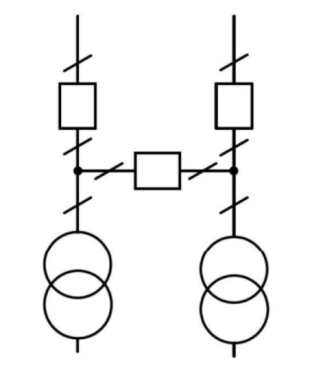
\includegraphics[width=0.2\textwidth]{inc/img/mostik}
	\caption{Схема РУ «мостик с выключателями в цепях линий»}
	\label{fig:мостик}
\end{figure}

\begin{figure}[ht]
	\centering
	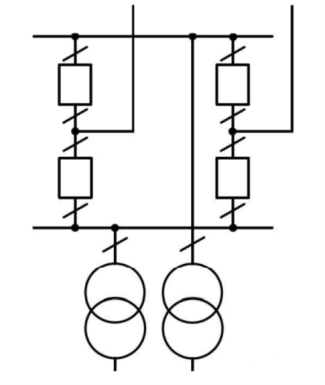
\includegraphics[width=0.2\textwidth]{inc/img/четырехугольник}
	\caption{Схема РУ «четырехугольник»}
	\label{fig:четырехугольник}
\end{figure}

\begin{figure}[ht]
	\centering
	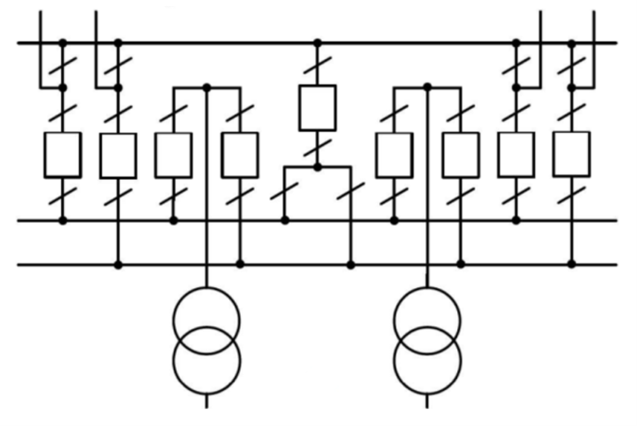
\includegraphics[width=0.4\textwidth]{inc/img/однорабоч_секц_с_обходкой}
	\caption{Схема РУ «одна рабочая секционированная выключателями и обходная системы шин с подключением трансформаторов к секциям шин через развилку из выключателей»}
	\label{fig:однарабоч_секц_с_обходкой}
\end{figure}

\begin{figure}[ht]
	\centering
	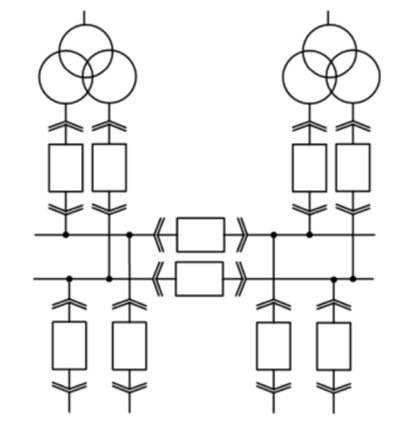
\includegraphics[width=0.2\textwidth]{inc/img/две_секц-ые_выключ}
	\caption{Схема РУ «две секционированные выключателями системы шин»}
	\label{fig:две_секц}
\end{figure}

\begin{figure}[ht]
	\centering
	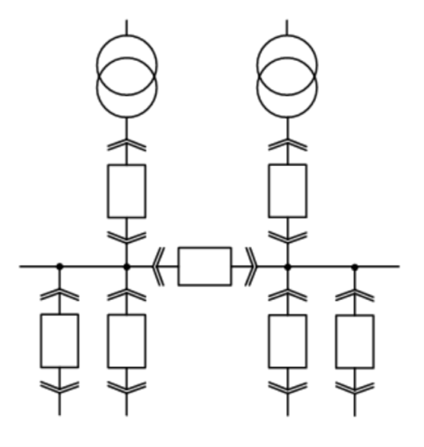
\includegraphics[width=0.2\textwidth]{inc/img/одна_секц-ая_выключ}
	\caption{Схема РУ «одна секционированная выключателем система шин»}
	\label{fig:одна_секц}
\end{figure}
\newpage
В качестве примера приведем расчет числа ячеек выключателей для варианта схемы сети 1. Для второго варианта схемы сети расчет выполняется аналогично. 
\subsection*{Тупиковая ПС5 110/10 кВ}

На стороне ВН применяется схема «мостик с выключателями в цепях линий» (рис. \ref{fig:мостик}), так как ПС5 тупиковая, и к ней присоединяются две трёхфазные цепи линий. Количество ячеек выключателей 110 кВ РУ ВН равно \(n_\textup{яч5}^{110} = 3\).


На стороне НН применяется схема «две секционированные выключателями системы шин» (рис. \ref{fig:две_секц}), поскольку на ПС5 установлено два трансформатора ТРДН-25000/110 с расщепленной обмоткой НН. Суммарное количество ячеек в цепях силовых трансформаторов и секционных выключателей \(n_\textup{яч.тр.и.св5}^{10} = 6\). Всего на шинах НН ПС5 установлено 8 БСК (см. табл. \ref{tab:нагрузки_с_батареями_кольцо} и табл. \ref{tab:первичная_компенсация}), подключаемых к каждой секции через 4 выключателя, т.е. общее число выключателей компенсирующих устройств \(n_\textup{яч.пс5}^\textup{БСК}=4\). Количество линий 10 кВ, отходящих от шин НН понижающих подстанций, примерно оценивается исходя из нагрузки подстанции и мощности, условно приходящейся на одну линию 10 кВ – 3,5 МВА \cite{глазунов_шведов}:
\begin{eqndesc}[H]
	\[n_\textup{кл5}^\textup{1секц} = \frac{S_\textup{нб5}}{3,5\cdot n_\textup{секц5}} = \frac{38,5}{3,5 \cdot 4} = 2,75,\]
где \(n_\textup{кл5}^\textup{1секц}\)- число линий, отходящих от одной секции РУ НН ПС5; \(n_\textup{секц5}\) – число секций в выбранной схеме РУ НН ПС5.
\end{eqndesc}

Округляем полученное значение \(n_\textup{кл5}^\textup{1секц}\) до ближайшего целого числа. Получаем \(n_\textup{кл5}^\textup{1секц}\) = 3, следовательно, количество ячеек выключателей отходящих линий 10 кВ будет: \(n_\textup{кл5}^{10} = n_\textup{кл5}^\textup{1секц}\cdot n_\textup{секц5} = 3\cdot 4 = 12\)

Итого получим суммарное количество ячеек выключателей 10 кВ РУ НН:
\[n_\textup{яч5}^{10} = n_\textup{яч.тр.и.св5}^{10} + n_\textup{яч.пс5}^\textup{БСК} + n_\textup{кл5}^{10} = 6 + 4 + 12 = 22\]

\subsection*{Проходные ПС1 и ПС2 220/10 кВ}

На стороне ВН применяется схема «четырехугольник» (рис. \ref{fig:четырехугольник}), так как ПС1 и ПС2 проходные и имеют 4 подключения со стороны ВН. Количество ячеек выключателей 220 кВ РУ ВН равно \(n_\textup{яч1}^{220} = 4\).

На стороне НН применяется схема «две секционированные выключателями системы шин» (рис. \ref{fig:две_секц}), поскольку на ПС1 и ПС2 установлено два трансформатора ТРДН-63000/220 с расщепленной обмоткой НН. Суммарное количество ячеек в цепях силовых трансформаторов и секционных выключателей \(n_\textup{яч.тр.и.св1}^{10} = 6\). Всего на шинах НН ПС1 и ПС2 установлено 8 БСК (см. табл. \ref{tab:нагрузки_с_батареями_кольцо} и табл. \ref{tab:первичная_компенсация}), подключаемых к каждой секции через 4 выключателя, т.е. общее число выключателей компенсирующих устройств \(n_\textup{яч.пс1}^\textup{БСК}=4\). Количество линий 10 кВ, отходящих от шин НН понижающих подстанций:
\[n_\textup{кл1}^\textup{1секц} = \frac{S_\textup{нб1}}{3,5\cdot n_\textup{секц1}} = \frac{76,1}{3,5 \cdot 4} = 5,43\]

Округляем полученное значение \(n_\textup{кл1}^\textup{1секц}\) до ближайшего целого числа. Получаем \(n_\textup{кл1}^\textup{1секц}\) = 5, следовательно, количество ячеек выключателей отходящих линий 10 кВ будет: \(n_\textup{кл1}^{10} = n_\textup{кл1}^\textup{1секц}\cdot n_\textup{секц1} = 5\cdot 4 = 20\)

Итого получим суммарное количество ячеек выключателей 10 кВ РУ НН:
\[n_\textup{яч1}^{10} = n_\textup{яч.тр.и.св1}^{10} + n_\textup{яч.пс1}^\textup{БСК} + n_\textup{кл1}^{10} = 6 + 4 + 20 = 30\]

\subsection*{Проходная ПС4 110/10 кВ}

На стороне ВН применяется схема «одна рабочая секционированная выключателями и обходная системы шин с подключением трансформаторов к секциям шин через развилку из выключателей» (рис. \ref{fig:однарабоч_секц_с_обходкой}), так как ПС4 проходная, и к ней присоединяются 2 двухцепные трёхфазные цепи линий. Количество ячеек выключателей 110 кВ РУ ВН равно \(n_\textup{яч4}^{110} = 9\).

На стороне НН применяется схема «две секционированные выключателями системы шин» (рис. \ref{fig:две_секц}), поскольку на ПС4 установлено два трансформатора ТРДН-40000/110 с расщепленной обмоткой НН. Суммарное количество ячеек в цепях силовых трансформаторов и секционных выключателей \(n_\textup{яч.тр.и.св4}^{10} = 6\). Всего на шинах НН ПС4 установлено 8 БСК (см. табл. \ref{tab:нагрузки_с_батареями_кольцо} и табл. \ref{tab:первичная_компенсация}), подключаемых к каждой секции через 4 выключателя, т.е. общее число выключателей компенсирующих устройств \(n_\textup{яч.пс4}^\textup{БСК}=4\). Количество линий 10 кВ, отходящих от шин НН понижающих подстанций:
\[n_\textup{кл1}^\textup{1секц} = \frac{S_\textup{нб1}}{3,5\cdot n_\textup{секц1}} = \frac{44,9}{3,5 \cdot 4} = 3,21\]

Округляем полученное значение \(n_\textup{кл4}^\textup{1секц}\) до ближайшего целого числа. Получаем \(n_\textup{кл4}^\textup{1секц}\) = 3, следовательно, количество ячеек выключателей отходящих линий 10 кВ будет: \(n_\textup{кл4}^{10} = n_\textup{кл4}^\textup{1секц}\cdot n_\textup{секц4} = 3\cdot 4 = 12\)

Итого получим суммарное количество ячеек выключателей 10 кВ РУ НН:
\[n_\textup{яч4}^{10} = n_\textup{яч.тр.и.св4}^{10} + n_\textup{яч.пс4}^\textup{БСК} + n_\textup{кл4}^{10} = 6 + 4 + 12 = 22\]

\subsection*{Автотрансформаторная ПС3 220/110/10 кВ}

На стороне ВН применяется схема «четырехугольник» (рис. \ref{fig:четырехугольник}), так как ПС3 проходная и к ней присоединяются две трехфазные цепи линии: \(n_\textup{яч3}^{220} = 4\).

На стороне СН применяется схема «одна рабочая секционированная выключателями и обходная система шин с подключением трансформаторов к секциям шин через развилку из выключателей» (рис. \ref{fig:однарабоч_секц_с_обходкой}). Общее количество присоединенных цепей линий – 2 (двухцепная линия 3-4).

Количество ячеек выключателей 110 кВ РУ CН складывается из 1 ячейки для обходной системы шин, из 2 ячеек на каждое присоединение автотрансформатора и 1 ячейки на каждую отходящую трёхфазную цепь. С учётом того, что подключается 2 автотрансформатора и 2 цепи линий, получаем 7 ячеек: \(n_\textup{яч3}^{110} = 1 + 4 + 2 = 7\)

На стороне НН применяется схема «одна секционированная выключателем система шин» (рис. \ref{fig:одна_секц}). Суммарное количество ячеек в цепях силовых трансформаторов и секционных выключателей \(n_\textup{яч.тр.и.св3}^{10}=3\), поскольку на ПС установлены автотрансформаторы, где отсутствует расщепление обмотки НН. Всего на шинах НН ПС3 установлено 4 компенсирующих устройства, равномерно распределим их, по 2 на каждую секцию, и тогда число выключателей компенсирующих устройств \(n_\textup{яч3}^\textup{БСК}=2\). Количество ячеек выключателей отходящих линий 10 кВ будет:
\[n_\textup{кл3}^\textup{1секц}=S_\textup{нб3}/(3,5\cdot n_\textup{секц1} )=\frac{33,0}{3,5\cdot 2}= 4,71\]

Округляем полученное значение \(n_\textup{кл3}^\textup{1секц}\) до ближайшего целого числа. Получаем  \(n_\textup{кл3}^\textup{1секц} = 5\), следовательно, количество ячеек выключателей отходящих линий 10 кВ:
\[n_\textup{кл3}^{10}=n_\textup{кл3}^\textup{1секц}\cdot n_\textup{секц1} = 5 \cdot 2 = 10\]

Итого получим суммарное количество ячеек выключателей 10 кВ РУ НН:
\[n_\textup{яч3}^\textup{10} = 3 + 2 + 10 = 15\]

Результаты расчетов числа ячеек выключателей РУ разных классов номинального напряжения для обоих вариантов схемы сети сведены в табл. \ref{tab:параметры_ру_схема_1} и \ref{tab:параметры_ру_схема_2}.

\begin{table}[h]
	\small
	\caption{Параметры РУ для варианта схемы сети 1}
	\label{tab:параметры_ру_схема_1}
	\begin{tabularx}{\linewidth}{|l|Z|Z|Z|Z|Z|Z|}
		\hline
		ПС         & 3(АТ)  & 1 & 2 & 4 & 5 & \multirow{4}{*}{ИТОГО:} \\ \cline{1-6}
		Схема РУВН & рис. \ref{fig:четырехугольник} & рис. \ref{fig:четырехугольник}  & рис. \ref{fig:четырехугольник} & рис. \ref{fig:однарабоч_секц_с_обходкой} & \ref{fig:мостик} & \\ \cline{1-6}
		Схема РУСН & рис. \ref{fig:однарабоч_секц_с_обходкой} & - & - & - & - & \\ \cline{1-6}
		Схема РУНН & рис. \ref{fig:одна_секц} & рис. \ref{fig:две_секц} & рис. \ref{fig:две_секц} & рис. \ref{fig:две_секц} & рис. \ref{fig:две_секц} & \\ \hline
		\(n_\textup{яч}^{220}\) & 4 & 4 & 4 & - & - & 12 \\ \hline
		\(n_\textup{яч}^{110}\) & 7 & - & - & 9 & 3 & 19 \\ \hline
		\(n_\textup{яч.тр.и.св}^{10}\) & 3 & 6 & 6 & 6 & 6 & \multirow{8}{*}{} \\ \cline{1-6}
		\(N_\textup{БСК}\) & 4 & 8 & 8 & 8 & 4 & \\ \cline{1-6}
		\(n_\textup{яч}^\textup{БСК}\) & 2 & 4 & 4 & 4 & 4 & \\ \cline{1-6}
		\(S_\textup{нб}\), МВА & 33,0 & 76,1 & 76,1 & 44,9 & 38,5 & \\ \cline{1-6}
		\(S_\textup{нб} / (3,5\cdot n_\textup{секц})\) & 4,71 & 5,43 & 5,43 & 3,21 & 2,75 & \\ \cline{1-6}
		\(n_\textup{кл}^\textup{1секц}\) & 5 & 5 & 5 & 3 & 3 & \\ \cline{1-6}
		Расщепление (секц.) & - (2) & + (4) & + (4) & + (4) & + (4) & \\ \cline{1-6}
		\(n_\textup{кл}^{10}\) & 10 & 20 & 20 & 12 & 12 & \\ \hline
		\(n_\textup{яч}^{10}\) & 15 & 30 & 30 & 22 & 22 & 119 \\ \hline
	\end{tabularx}
\end{table}

\begin{table}[H]
	\small
	\caption{Параметры РУ для варианта схемы сети 2}
	\label{tab:параметры_ру_схема_2}
	\begin{tabularx}{\linewidth}{|l|Z|Z|Z|Z|Z|Z|}
		\hline
		ПС         & 3(АТ)  & 1 & 2 & 4 & 5 & \multirow{4}{*}{ИТОГО:} \\ \cline{1-6}
		Схема РУВН & рис. \ref{fig:четырехугольник} & рис. \ref{fig:однарабоч_секц_с_обходкой}  & рис. \ref{fig:мостик} & рис. \ref{fig:однарабоч_секц_с_обходкой} & \ref{fig:мостик} & \\ \cline{1-6}
		Схема РУСН & рис. \ref{fig:однарабоч_секц_с_обходкой} & - & - & - & - & \\ \cline{1-6}
		Схема РУНН & рис. \ref{fig:одна_секц} & рис. \ref{fig:две_секц} & рис. \ref{fig:две_секц} & рис. \ref{fig:две_секц} & рис. \ref{fig:две_секц} & \\ \hline
		\(n_\textup{яч}^{220}\) & 4 & 9 & - & - & - & 13 \\ \hline
		\(n_\textup{яч}^{110}\) & 9 & - & 3 & 9 & 3 & 24 \\ \hline
		\(n_\textup{яч.тр.и.св}^{10}\) & 3 & 6 & 6 & 6 & 6 & \multirow{8}{*}{} \\ \cline{1-6}
		\(N_\textup{БСК}\) & 4 & 10 & 10 & 10 & 6 & \\ \cline{1-6}
		\(n_\textup{яч}^\textup{БСК}\) & 2 & 4 & 4 & 4 & 4 & \\ \cline{1-6}
		\(S_\textup{нб}\), МВА & 33,0 & 76,1 & 76,1 & 44,9 & 38,5 & \\ \cline{1-6}
		\(S_\textup{нб} / (3,5\cdot n_\textup{секц})\) & 4,71 & 5,43 & 5,43 & 3,21 & 2,75 & \\ \cline{1-6}
		\(n_\textup{кл}^\textup{1секц}\) & 5 & 5 & 5 & 3 & 3 & \\ \cline{1-6}
		Расщепление (секц.) & - (2) & + (4) & + (4) & + (4) & + (4) & \\ \cline{1-6}
		\(n_\textup{кл}^{10}\) & 10 & 20 & 20 & 12 & 12 & \\ \hline
		\(n_\textup{яч}^{10}\) & 15 & 30 & 30 & 22 & 22 & 119 \\ \hline
	\end{tabularx}
\end{table}


%%% Local Variables:
%%% mode: latex
%%% TeX-master: "rpz"
%%% End:
\chapter{Выбор рационального варианта схемы сети}
\label{cha:рациональная_схема}

На данном этапе проектирования из числа сформированных вариантов схем сети необходимо выбрать наиболее рациональный. Данный раздел проектирования заключается в технико-экономическом сопоставлении рассматриваемых вариантов. Рекомендуется двухэтапное сопоставление рассматриваемых вариантов.

\textit{Сравнение количественных натуральных показателей}

На данном этапе варианты с одинаковым номинальным напряжением сопоставляются по натуральным количественным показателям, отражающим капиталовложения, а, следовательно, и эксплуатационные расходы по сети. Такими показателями являются:
\begin{itemize}
	\item протяженность трасс линий;
	\item протяженность линий в одноцепном исчислении;
	\item суммарные количества ячеек выключателей разных классов напряжения на подстанциях сети.
\end{itemize}

Натуральные количественные показатели для двух рассматриваемых вариантов схемы сети представлены в таблице \ref{tab:натур_показатели}

\begin{table}[H]
	\small
	\caption{Натуральные количественные показатели для обоих вариантов схемы сети}
	\label{tab:натур_показатели}
	\begin{tabularx}{\linewidth}{|Z|Z|Z|Z|Z|}
		\hline
		\multicolumn{2}{|c|}{Cхема №} & 1 & 2 & Лучший показатель \\ \hline
		\multirow{2}{*}{220 кВ} & Протяженность трасс ЛЭП & 182 & 91 & 2\\ \cline{2-5}
		                        & Протяженность цепей & 182 & 182 & 1, 2 \\ \hline
		 \multirow{2}{*}{110 кВ} & Протяженность трасс ЛЭП & 51,8 & 51,8 & 1,2 \\ \cline{2-5}
		 					     & Протяженность цепей & 103,6 & 103,6 & 1, 2 \\ \hline
		 \multicolumn{2}{|c|}{Выключатели 220} & 12 & 13 & 1 \\ \hline
		 \multicolumn{2}{|c|}{Выключатели 110} & 19 & 24 & 1 \\ \hline
		 \multicolumn{2}{|c|}{Выключатели 10} & 119 & 119 & 1, 2 \\ \hline 
	\end{tabularx}
\end{table}

\section{Технико-экономическое сопоставление}

На данном этапе проводится технико-экономическое сопоставление вариантов схем сети в их различающихся частях. Одним из основных показателей экономической эффективности проекта является чистый дисконтированный доход (ЧДД) за расчетный период, приведенный к году начала реализации проекта (первому году):
\begin{eqndesc}[h]
	\begin{equation*}
		\textup{ЧДД} = \sum_{t=1}^{T_\textup{р}} [(\textup{Д}_t - \textup{З}_t)(1 + E)^{1-t}],
		\label{eqn:чдд}
	\end{equation*}
где \(\textup{Д}_t\) "--- величина дохода в год \textit{t}; \(\textup{З}_t\) "--- величина затрат в год \textit{t}; \textit{E} "--- норматив дисконтирования, \(E = 0,1\); \(T_\textup{р}\) "--- расчетный период (\(T_\textup{р} = 10\) лет).
\end{eqndesc}

Проект считается экономически эффективным, если его ЧДД больше нуля, при выборе между несколькими вариантами предпочтение отдается варианту с более высоким ЧДД. Так как все варианты имеют одинаковый производственный эффект, т.е. \(\textup{Д}_{t1} = \textup{Д}_{t2}\), сравнение сводится к сравнению дисконтированных затрат за расчетный период:
\begin{eqndesc}[h]
	\begin{equation}
		\textup{З}_\textup{д} = D_\textup{р}\cdot \textup{К}_\Sigma + D_\textup{д}\cdot \textup{И}_{\textup{пот}\Sigma},
		\label{eqn:упрощ.формула_затрат}
	\end{equation}
где \(D_\textup{р}\) "--- расчетный множитель; \(D_\textup{д}\) "--- дисконтирующий множитель; \(\textup{К}_\Sigma\) "--- суммарные капиталовложения в сеть; \(\textup{И}_{\textup{пот}\Sigma}\) "--- суммарные ежегодные издержки на возмещение потерь электроэнергии.
\end{eqndesc}

\textit{Различия вариантов схем сети 1 и 2}

\begin{itemize}
	\item одноцепные линии 220 кВ: К-1, К-2, 1-3, 2-3 (схема варианта сети 1)
	\item двухцепные линии 220 кВ: К-1, 1-3 (схема варианта сети 2)
	\item двухцепная линия 110 кВ: 3-2 (схема варианта сети 2)
	\item РУВН на подстанциях 1 и 2
	\item трансформаторное оборудование на подстанциях 2 и 3
	\item дополнительное оборудования в виде компенсирующих устройств на каждой подстанции
\end{itemize}

Капиталовложения на сооружение линии электропередачи:
\begin{equation*}
	\textup{К}_\textup{ЛЭП} = \textup{К}_{0\textup{ЛЭП.баз}}\cdot k_\textup{зон}\cdot k_\textup{усл}\cdot k_\textup{деф}\cdot L,
	\label{eqn:капиталовложения_лэп}
\end{equation*}
где \(\textup{К}_{0\textup{ЛЭП.баз}}\) "--- укрупненный показатель стоимости сооружения 1 км воздушной линии; \(k_\textup{зон} = 1,0\) "--- учитывающий удорожание строительства ВЛ в Центре; \(k_\textup{усл} = 1\) "--- коэффициент усложняющих условий строительства, в отсутствии данных принимается равным единице; \(k_\textup{деф} = 4,25\) "--- коэффииент дефляции показывает приведение цен базового года к ценам 2010 года.

Для линии К-1 варианта схемы сети 1:
\[\textup{К}_\textup{ЛЭП.К-1} = 1188\cdot 1,0\cdot 1,0\cdot 4,25\cdot 41,8 = 211048,2 \textup{тыс. руб}\]

Капиталовложения в остальные линии для вариантов схем сети 1 и 2 рассчитываются аналогично, результаты расчетов представлены в таблицах \ref{tab:капиталовложения_лэп_1} и \ref{tab:капиталовложения_лэп_2} соответственно.

\begin{table}[h]
	\small
	\caption{Капиталовложения на сооружение ЛЭП для варианта схемы сети 1}
	\label{tab:капиталовложения_лэп_1}
	\begin{tabularx}{\linewidth}{|Z|Z|Z|Z|Z|Z|}
		\hline
		ЛЭП & К-1 & К-2 & 1-3 & 2-3 & Итого \\ \hline
		\(U_\textup{ном}\), кВ & 220 & 220 & 220 & 220 & - \\ \hline
		\(F,\; \textup{мм}^2\) & 400 & 400 & 240 & 240 & - \\ \hline
		\(n_\textup{ц}\) & 1 & 1 & 1 & 1 & - \\ \hline
		\(\textup{К}_{0\textup{ЛЭП.баз}\; \frac{\textup{тыс.руб}}{км}}\) & 1188 & 1188 & 990 & 990 & - \\ \hline
		\(L_{i-j}\), км & 41,8 & 49,2 & 49,2 & 41,8 & - \\ \hline
		\(\textup{К}_\textup{ЛЭП}\), тыс. руб & 211048,2 & 248419,8 & 207009,0 & 175873,5 & 842341,5 \\ \hline
	\end{tabularx}
\end{table}

\begin{table}[h]
	\small
	\caption{Капиталовложения на сооружение ЛЭП для варианта схемы сети 2}
	\label{tab:капиталовложения_лэп_2}
	\begin{tabularx}{\linewidth}{|Z|Z|Z|Z|Z|}
		\hline
		ЛЭП & К-1 & 1-3 & 2-3 & Итого \\ \hline
		\(U_\textup{ном}\), кВ & 220 & 220 & 110 & - \\ \hline
		\(F,\; \textup{мм}^2\) & 400 & 300 & 240 & - \\ \hline
		\(n_\textup{ц}\) & 2 & 2 & 2  & - \\ \hline
		\(\textup{К}_{0\textup{ЛЭП.баз}}\; \frac{\textup{тыс.руб}}{\textup{км}}\) & 2219 & 2020 & 1403  & - \\ \hline
		\(L_{i-j}\), км & 41,8 & 49,2 & 41,8  & - \\ \hline
		\(\textup{К}_\textup{ЛЭП}\), тыс. руб & 394205,35 & 422382,0 & 249242,95 & 1065830,3 \\ \hline
	\end{tabularx}
\end{table}

Капиталовложения на сооружение подстанций:
\begin{eqndesc}[h]
	\begin{equation*}
		\textup{К}_\textup{ПС} = \textup{К}_{\textup{ТР}\Sigma} + \textup{К}_{\textup{РУ}\Sigma} + \textup{К}_{\textup{доп}\Sigma} + \textup{К}_{\textup{пост}},
		\label{eqn:капит_на_сооруж_пс}
	\end{equation*}
где \(\textup{К}_{\textup{ТР}\Sigma}\) "--- стоимость устанавливаемых трансформаторов (автотрансформаторов), тыс. руб; \(\textup{К}_{\textup{РУ}\Sigma}\) "--- суммарная стоимость РУ всех классов напряжения, тыс. руб; \(\textup{К}_{\textup{доп}\Sigma}\) "--- суммарная стоимость дополнительного оборудования, тыс. руб; \(\textup{К}_{\textup{пост}}\) "--- постоянная часть затрат на сооружение ПС, тыс. руб.
\end{eqndesc}

В курсовом проекте принимаем, что при напряжениях 220 и 110 кВ используются воздушные выключатели, а при 10 кВ - вакуумные \cite{глазунов_шведов}

В качестве примера приведем расчет капиталовложений для ПС2.

\textit{Трансформаторы}

В первой и втором варианте схемы отличается класс уровня напряжения трансформатора (ТРДН-63000/220 и ТРДН-63000/110 соответственно), установленные на ПС2. Капиталовложения для каждой пары ячеек трансформаторов рассчитываются по формуле:
	\begin{equation*}
		\textup{К}_\textup{ТР} = \textup{К}_\textup{тр.баз}\cdot k_\textup{зон}\cdot k_\textup{деф}\cdot n_\textup{т},
	\end{equation*}
где \(\textup{К}_\textup{тр.баз}\) "--- базовый укрупненный показатель стоимости ячейки автотрансформаторов, тыс. руб; \(n_\textup{т}\) "--- число трансформаторов, установленных на ПС.

\[\textup{К}_\textup{ТР2(1)} = \textup{К}_\textup{тр.баз.220}\cdot k_\textup{зон}\cdot k_\textup{деф}\cdot n_\textup{т} = 12625\cdot 1\cdot 4,25\cdot 2 = 107312,5\; \textup{тыс. руб}\]
\[\textup{К}_\textup{ТР2(2)} = \textup{К}_\textup{тр.баз.110}\cdot k_\textup{зон}\cdot k_\textup{деф}\cdot n_\textup{т} = 9000\cdot 1\cdot 4,25\cdot 2 = 76500,0\; \textup{тыс. руб}\]

\textit{Схемы РУ}

На ПС2 в двух вариантах схем сети отличаются схемы РУВН, для первой схемы это "четырехугольник", а для второй схемы сети "мостик". Капиталовложения постоянной части затрат ПС2:
	\begin{equation*}
		\textup{К}_\textup{пост} = \textup{К}_\textup{пост.баз}\cdot k_\textup{зон}\cdot k_\textup{деф},
	\end{equation*}
где \(\textup{К}_\textup{пост.баз}\) "--- базовый укрупненный показатель постоянной части затрат на сооружение ПС в базисных ценах на 01.01.2000 г. для европейской части РФ.
\[\textup{К}_\textup{пост(1)} = \textup{К}_\textup{пост.баз.220}\cdot k_\textup{зон}\cdot k_\textup{деф} = 19500\cdot 1\cdot 4,25 = 82875\; \textup{тыс. руб}\]
\[\textup{К}_\textup{пост(2)} = \textup{К}_\textup{пост.баз.110}\cdot k_\textup{зон}\cdot k_\textup{деф} = 9000\cdot 1\cdot 4,25 = 38250\; \textup{тыс. руб}\]

Разница в ячейках рассчитывается по формуле:
\[\textup{К}_\textup{РУ} = \textup{К}_\textup{выкл.баз}\cdot k_\textup{зон}\cdot k_\textup{деф}\cdot n_\textup{яч},\]
где \(\textup{К}_\textup{выкл.баз}\) "--- базовый укрупненный показатель стоимость ячейки выключателя в базисных ценах на 01.01.2000 для европейской части РФ.
\[\textup{К}_\textup{РУВН(1)} = \textup{К}_\textup{выкл.баз.220(1)}\cdot k_\textup{зон}\cdot k_\textup{деф}\cdot n_\textup{яч}^\textup{220} = 8800\cdot 4,25\cdot 4 = 149600\; \textup{тыс. руб}\]
\[\textup{К}_\textup{РУВН(2)} = \textup{К}_\textup{выкл.баз.110(2)}\cdot k_\textup{зон}\cdot k_\textup{деф}\cdot n_\textup{яч}^\textup{220} = 4150\cdot 4,25\cdot 3 = 52912,5\; \textup{тыс. руб}\]

\textit{Дополнительное оборудование}

В первом варианте схемы сети предполагается установка 8 БСК на ПС2, а во втором варианте схемы сети 10 БСК. Дополнительные капиталовложения в дополнительное оборудование для варианта схемы сети 2:
\[\textup{К}_\textup{доп2(2)} = \textup{К}_\textup{БСК.баз}\cdot k_\textup{зон}\cdot k_\textup{деф}\cdot (n_\textup{БСК1} - n_\textup{БСК2})\]
где \(\textup{К}_\textup{БСК.баз}\) "--- укрупненная стоимость шунтовой конденсаторной батареи 10 кВ единичной мощностью 1,2 МВар; \(n_\textup{БСК1}\) "--- общее число КУ, установленных в 1 варианте схемы сети; \(n_\textup{БСК2}\) "--- общее число КУ, установленных во 2 варианте схемы сети.
\[\textup{К}_\textup{доп2(2)} = \textup{К}_\textup{БСК.баз}\cdot k_\textup{зон}\cdot k_\textup{деф}\cdot (n_\textup{БСК1} - n_\textup{БСК2}) = 375\cdot 425\cdot (10-8) = 3187,5\; \textup{тыс. руб}\]

Для остальных ПС с различной стоимостью составляющих в двух вариантах схемы сети расчет проводится аналогично. Результаты расчетов различной стоимости ПС вместе с капиталовложениями в ЛЭП сведем в табл. \ref{tab:сравнение_схем}.

%\begin{table}
%	\small
{\small
	\begin{xltabular}{\linewidth}{|Z|Z|Z|Z|Z|}		
		\caption{Сравнение вариантов схем сети по стоимости ЛЭП и ПС} 
		\label{tab:сравнение_схем} \\ \hline
		\multicolumn{5}{|c|}{ЛЭП} \\ 
		\endfirsthead
		\caption{\textit{(Продолжение)} Сравнение вариантов схем сети по стоимости ЛЭП и ПС}\\
		\hline
		\endhead
		\multicolumn{5}{r}{\textit{Продолжение на следующей странице}} \\
		\endfoot
		\endlastfoot
		\hline
		Вариант & Линия & \(\textup{К}_{0\textup{ЛЭП.баз}}\), тыс. руб/км & \(\textup{К}_\textup{ЛЭП}\), тыс. руб & \(\textup{К}_{\textup{ЛЭП}\Sigma}\), тыс. руб \\ \hline
		\multirow{4}{*}{№ 1} & К-1 & 1188 & 211048,2 & \multirow{4}{*}{842348,5} \\ \cline{2-4}
		                     & К-2 & 1188 & 248419,8 &                           \\ \cline{2-4}
		                     & 1-3 & 990  & 207009,0 &                           \\ \cline{2-4}
		                     & 2-3 & 990  & 175873,5 &                           \\ \hline
		\multirow{3}{*}{№ 2} & К-1 & 2219 & 394205,4 & \multirow{3}{*}{1065830,3}\\ \cline{2-4}
		                     & 1-3 & 2020 & 422382,0 &                           \\ \cline{2-4}
		                     & 2-3 & 1403 & 249243,0 &                           \\ \hline
		 \multicolumn{5}{|c|}{ПС2} \\ \hline
		 Вариант & \multicolumn{2}{c|}{Тип ТР} & \(\textup{К}_\textup{тр.баз}\), тыс. руб & \(\textup{К}_\textup{ТР.2}\), тыс. руб \\ \hline
		 № 1 & \multicolumn{2}{c|}{ТРДН-63000/220} & 12625 & 107312,5 \\ \hline
		 № 2 & \multicolumn{2}{c|}{ТРДН-63000/110} & 9000  & 76500,0  \\ \hline
		 \multicolumn{5}{|c|}{РУВН ПС2} \\ \hline
		 Вариант & \multicolumn{2}{c|}{\(n_\textup{яч}\)} & \(\textup{К}_\textup{выкл. баз}\), тыс. руб & \(\textup{К}_\textup{РУВН2}\), тыс. руб \\ \hline
		 № 1 & \multicolumn{2}{c|}{4} & 8800 & 149600 \\ \hline
		 № 2 & \multicolumn{2}{c|}{3} & 4150 & 52912,5 \\ \hline
		 \multicolumn{5}{|c|}{Дополнительное оборудование ПС2} \\ \hline
		 Вариант & \multicolumn{2}{c|}{\(N_\textup{БСК}\)} & \(\textup{К}_\textup{БСК.баз}\), тыс. руб & \(\textup{К}_\textup{доп2(2)}\), тыс. руб \\ \hline
		 № 1 & \multicolumn{2}{c|}{8} & 375 & - \\ \hline
		 № 2 & \multicolumn{2}{c|}{10} & 375 & 3187,5 \\ \hline
		 \multicolumn{5}{c|}{Постоянная часть затрат на сооружение ПС2} \\ \hline
		 Вариант & \multicolumn{2}{c|}{Схема РУВН (ВН/НН)} & \(\textup{К}_\textup{пост.баз}\), тыс. руб & \(\textup{К}_\textup{пост2}\), тыс. руб. \\ \hline
		 № 1 & \multicolumn{2}{c|}{Четырехугольник (220/10)} & 19500 & 82875 \\ \hline
		 № 2 & \multicolumn{2}{c|}{Мостик (110/10)} & 9000 & 38250 \\ \hline
		 \multicolumn{5}{|c|}{ПС3} \\ \hline
		 Вариант & \multicolumn{2}{c|}{Тип ТР} & \(\textup{К}_\textup{тр.баз}\), тыс. руб & \(\textup{К}_\textup{ТР.3}\), тыс. руб \\ \hline
		 № 1 & \multicolumn{2}{c|}{АТДЦТН-125000/220/110} & 15525 & 131962,5 \\ \hline
		 № 2 & \multicolumn{2}{c|}{АТДЦТН-200000/220/110} & 21050 & 178925,0 \\ \hline
		 \multicolumn{5}{|c|}{РУCН ПС3} \\ \hline
		 Вариант & \multicolumn{2}{c|}{\(n_\textup{яч}^{110}\)} & \(\textup{К}_\textup{выкл. баз}\), тыс. руб & \(\textup{К}_\textup{РУСН3(2)}\), тыс. руб \\ \hline
		 № 1 & \multicolumn{2}{c|}{7} & 4150 & - \\ \hline
		 № 2 & \multicolumn{2}{c|}{9} & 4150 & 35275 \\ \hline
		 \multicolumn{5}{|c|}{ПС1} \\ \hline
		  \multicolumn{5}{|c|}{Постоянная часть затрат на сооружение ПС1} \\ \hline
		 Вариант & \multicolumn{2}{c|}{Схема РУВН (ВН/НН)} & \(\textup{К}_\textup{пост.баз}\), тыс. руб & \(\textup{К}_\textup{пост1}\), тыс. руб. \\ \hline
		 № 1 & \multicolumn{2}{c|}{Четырехугольник (220/10)} & 19500 & - \\ \hline
		 № 2 & \multicolumn{2}{c|}{Сборные шины (220/10)} & 19500 & - \\ \hline
		 \multicolumn{5}{|c|}{Дополнительное оборудование ПС1} \\ \hline
		 Вариант & \multicolumn{2}{c|}{\(N_\textup{БСК}\)} & \(\textup{К}_\textup{БСК.баз}\), тыс. руб & \(\textup{К}_\textup{доп1(2)}\), тыс. руб \\ \hline
		 № 1 & \multicolumn{2}{c|}{8} & 375 & - \\ \hline
		 № 2 & \multicolumn{2}{c|}{10} & 375 & 3187,5 \\ \hline
		 \multicolumn{5}{|c|}{ПС4} \\ \hline
		 \multicolumn{5}{|c|}{Дополнительное оборудование ПС4} \\ \hline
		 Вариант & \multicolumn{2}{c|}{\(N_\textup{БСК}\)} & \(\textup{К}_\textup{БСК.баз}\), тыс. руб & \(\textup{К}_\textup{доп4(2)}\), тыс. руб \\ \hline
		 № 1 & \multicolumn{2}{c|}{8} & 375 & - \\ \hline
		 № 2 & \multicolumn{2}{c|}{10} & 375 & 3187,5 \\ \hline
		 \multicolumn{5}{|c|}{ПС5} \\ \hline
		 \multicolumn{5}{|c|}{Дополнительное оборудование ПС5} \\ \hline
		 Вариант & \multicolumn{2}{c|}{\(N_\textup{БСК}\)} & \(\textup{К}_\textup{БСК.баз}\), тыс. руб & \(\textup{К}_\textup{доп5(1)}\), тыс. руб \\ \hline
		 № 1 & \multicolumn{2}{c|}{8} & 375 & 3187,5 \\ \hline
		 № 2 & \multicolumn{2}{c|}{6} & 375 & - \\ \hline
		 \multicolumn{5}{|c|}{Итого} \\ \hline
		 Вариант & \multicolumn{2}{c|}{\(\textup{К}_{\textup{ЛЭП}\Sigma}\), тыс. руб.} & \(\textup{К}_{\textup{ПС.220}\Sigma}\), тыс. руб & \(\textup{К}_{\textup{ПС.110}\Sigma}\), тыс. руб \\ \hline
		 № 1 & \multicolumn{2}{c|}{842348,5} & 471750,0 & 3187,5 \\ \hline
		 № 2 & \multicolumn{2}{c|}{1065830,3} & 178925,0 & 212500,0 \\ \hline
	\end{xltabular}
}
%\end{table}

\textit{Издержки на возмещение потерь электроэнергии}

Приведем пример расчета нагрузочных потерь активной мощности для линии К-1 схемы:
\[\Delta P_{K-1} = \frac{S_{K-1}^2\cdot R_{K-1}}{U_\textup{ном}^2} = \frac{134,9^2\cdot 3,05}{220^2} = 1,15\; \textup{МВт}\]

Расчет для других линий вариантов схемы сети 1 и 2 проведен аналогично. Результаты расчета сведены в таблицы \ref{tab:нагр_потери_1} и \ref{tab:нагр_потери_2}.

\begin{table}[h]
	\small
	\caption{Нагрузочные потери в линиях для варианта схемы сети 1}
	\label{tab:нагр_потери_1}
	\begin{tabularx}{\linewidth}{|Z|Z|Z|Z|Z|Z|Z|Z|}
		\hline
		Линия                           & К-1   & К-2   & 1-3  & 2-3  & 3-4  & 4-5  & Итого \\ \hline
		\textit{S}, МВА                          & 134,9 & 129,0 & 60,3 & 54,4 & 80,2 & 37,7 &  -    \\ \hline
		\(R_\textup{л}\), Ом            & 3,05  & 3,59  & 5,81 & 4,93 & 1,53 & 3,16 &  -    \\ \hline
		\(\Delta P_\textup{л(1)}\), МВт & 1,15  & 1,23  & 0,44 & 0,30 & 0,81 & 0,37 & 4,30  \\ \hline
	\end{tabularx}
\end{table}

\begin{table}[h]
	\small
	\caption{Нагрузочные потери в линиях для варианта схемы сети 1}
	\label{tab:нагр_потери_2}
	\begin{tabularx}{\linewidth}{|Z|Z|Z|Z|Z|Z|Z|}
		\hline
		Линия                           & К-1   & 1-3   & 3-2  & 3-4  & 4-5  & Итого \\ \hline
		\textit{S}, МВА                          & 262,5 & 188,7 & 73,9 & 78,6 & 36,9 &  -    \\ \hline
		\(R_\textup{л}\), Ом            & 1,53  & 2,36  & 2,47 & 1,53 & 3,16 &  -    \\ \hline
		\(\Delta P_\textup{л(1)}\), МВт & 2,18  & 1,73  & 1,11 & 0,78 & 0,36 & 6,17  \\ \hline
	\end{tabularx}
\end{table}

В соответствии с исходными данными время наибольших нагрузок \(T_\textup{нб} = 4350\; \frac{\textup{ч}}{\textup{год}}\). Тогда время наибольших потерь:
\[\tau = \frac{1}{3}\cdot T_\textup{нб} + \frac{2}{3}\cdot \frac{T_\textup{нб}^2}{8760} = \frac{1}{3}\cdot 4350 + \frac{2}{3}\cdot \frac{4350^2}{8760} = 2890,1\; \frac{\textup{ч}}{\textup{год}}\]

Рассчитаем нагрузочные потери активной мощности в трансформаторах: 2xТРДН-63000/220 для варианта схемы сети 1 и 2xТРДН-63000/110 для варианта схемы сети 2, установленных на ПС2 (с учетом компенсации реактивной мощности):
\[\Delta P_\textup{Т2(1)} = \frac{S_\textup{нб2}^{''2}\cdot R_\textup{Т2(1)}}{U_\textup{ном}^2\cdot n_\textup{т}} = \frac{72,9^2\cdot 3,9}{220^2\cdot 2} = 0,214\; \textup{МВт};\]
\[\Delta P_\textup{Т2(2)} = \frac{S_\textup{нб2}^{''2}\cdot R_\textup{Т2(2)}}{U_\textup{ном}^2\cdot n_\textup{т}} = \frac{72,2^2\cdot 0,87}{110^2\cdot 2} = 0,187\; \textup{МВт},\]
где \(R_\textup{т(1)}\) и \(R_\textup{т(2)}\) "--- активные сопротивления обмоток трансформаторов ТРДН-63000/220 и ТРДН-63000/110 соответственно.

Проведем расчет нагрузочных потерь активной мощности в двух автотрансформаторах АТДЦТН-125000/220/110, установленных на ПС3, для варианта схемы сети 1 (с учетом компенсации реактивной мощности):
\[\Delta P_\textup{ат3(1)ВН} = \frac{S_\textup{нб.ВН(1)}^{''2}\cdot R_\textup{ат3(ВН)}}{U_\textup{ном}^2\cdot n_\textup{ат}} = \frac{111,4^2\cdot 0,5}{220^2\cdot 2} = 0,0641\; \textup{МВт};\]
\[\Delta P_\textup{ат3(1)CН} = \frac{S_\textup{нб.CН(1)}^{''2}\cdot R_\textup{ат3(CН)}}{U_\textup{ном}^2\cdot n_\textup{ат}} = \frac{80,2^2\cdot 0,5}{220^2\cdot 2} = 0,0332\; \textup{МВт};\]
\[\Delta P_\textup{ат3(1)НН} = \frac{S_\textup{нб.НН(1)}^{''2}\cdot R_\textup{ат3(НН)}}{U_\textup{ном}^2\cdot n_\textup{ат}} = \frac{31,3^2\cdot 1}{220^2\cdot 2} = 0,0101\; \textup{МВт},\]
где \(R_\textup{т.нн}\), \(R_\textup{т.сн}\) и \(R_\textup{т.вн}\) "--- каталожные данные по активным сопротивлениям обмоток автотрансформатора АТДЦТН-125000/220/110 \cite{файбисович}.
\[\Delta P_\textup{ат(1)} = \Delta P_\textup{ат3(1)ВН} + \Delta P_\textup{ат3(1)CН} + \Delta P_\textup{ат3(1)НН} =\] \[= 0,0641 + 0,0332 + 0,0101 = 0,107\; \textup{МВт}\]

Проведем расчет нагрузочных потерь активной мощности в двух автотрансформаторах АТДЦТН-200000/220/110, установленных на ПС3, для варианта схемы сети 2 (с учетом компенсации реактивной мощности):
\[\Delta P_\textup{ат3(2)ВН} = \frac{S_\textup{нб.ВН(2)}^{''2}\cdot R_\textup{ат3(ВН)}}{U_\textup{ном}^2\cdot n_\textup{ат}} = \frac{183,8^2\cdot 0,3}{220^2\cdot 2} = 0,105\; \textup{МВт};\]
\[\Delta P_\textup{ат3(2)CН} = \frac{S_\textup{нб.CН(2)}^{''2}\cdot R_\textup{ат3(CН)}}{U_\textup{ном}^2\cdot n_\textup{ат}} = \frac{152,4^2\cdot 0,3}{220^2\cdot 2} = 0,0720\; \textup{МВт};\]
\[\Delta P_\textup{ат3(2)НН} = \frac{S_\textup{нб.НН(ц)}^{''2}\cdot R_\textup{ат3(НН)}}{U_\textup{ном}^2\cdot n_\textup{ат}} = \frac{31,3^2\cdot 0,6}{220^2\cdot 2} = 0,0061\; \textup{МВт},\]
где \(R_\textup{т.нн}\), \(R_\textup{т.сн}\) и \(R_\textup{т.вн}\) "--- каталожные данные по активным сопротивлениям обмоток автотрансформатора АТДЦТН-200000/220/110 \cite{файбисович}.
\[\Delta P_\textup{ат(2)} = \Delta P_\textup{ат3(2)ВН} + \Delta P_\textup{ат3(2)CН} + \Delta P_\textup{ат3(2)НН} =\] \[=0,105 + 0,0720 + 0,0061 = 0,183\; \textup{МВт}\]

Суммарные годовые нагрузочные потери электроэнергии для вариантов схемы сети 1 и 2:
\[\Delta \textup{Э}_\textup{нагр(1)} = \Delta P_{(1)}\cdot \tau = (\Delta P_\textup{л(1)} + \Delta P_\textup{Т2(1)} + \Delta P_\textup{ат(1)})\cdot \tau =\] \[= (4,30 + 0,214 + 0,107)\cdot 2890,1 = 13355,2\; \frac{\textup{МВт}\cdot \textup{ч}}{\textup{год}}\]
\[\Delta \textup{Э}_\textup{нагр(2)} = \Delta P_{(2)}\cdot \tau = (\Delta P_\textup{л(2)} + \Delta P_\textup{Т2(2)} + \Delta P_\textup{ат(2)})\cdot \tau =\] \[= (6,17 + 0,187 + 0,183)\cdot 2890,1 = 18901,3\; \frac{\textup{МВт}\cdot \textup{ч}}{\textup{год}}\]

\textit{Условно-постоянные потери активной мощности}

Разница между схемами сети 1 и 2 будет состоять в потерях в стали силовых ТР на ПС3 и ПС2, так как там разные ТР. Величина условно постоянных потерь для вариантов схемы сети 1 и 2 будет определяться:
\[\Delta P_\textup{усл.пост(1)} = \Delta P_\textup{х.экв.тр2(1)} + \Delta P_\textup{х.экв.ат3(1)} = 82\cdot 2 + 85\cdot 2 = 310\; \textup{кВт} = 0,334\; \textup{МВт};\]
\[\Delta P_\textup{усл.пост(2)} = \Delta P_\textup{х.экв.тр2(2)} + \Delta P_\textup{х.экв.ат3(2)} = 59\cdot 2 + 125\cdot 2 = 310\; \textup{кВт} = 0,368\; \textup{МВт},\]
где \(\Delta P_\textup{х.экв.тр2(1)}\) и \(\Delta P_\textup{х.экв.тр2(2)}\) "--- каталожные данные по потерям холостого хода трансформаторов ТРДН-63000/220 и ТРДН-63000/110 соответственно; \(\Delta P_\textup{х.экв.ат3(1)}\) и \(\Delta P_\textup{х.экв.ат3(2)}\) "--- каталожные данные по потерям холостого хода автотрансформаторов АТДЦТН-125000/220/110 и АТДЦТН-200000/220/110 соответственно, приведенные в справочнике \cite{файбисович}.

Суммарные годовые условно-постоянные потери электроэнергии для вариантов схемы сети 1 и 2:
\[\Delta \textup{Э}_{\textup{усл.пост(1)}\Sigma} = \Delta P_\textup{усл.пост(1)}\cdot T_\textup{год} = 0,334\cdot 8760 = 2925,8\; \frac{\textup{МВт}\cdot \textup{ч}}{\textup{год}}\]
\[\Delta \textup{Э}_{\textup{усл.пост(2)}\Sigma} = \Delta P_\textup{усл.пост(2)}\cdot T_\textup{год} = 0,368\cdot 8760 = 3223,7\; \frac{\textup{МВт}\cdot \textup{ч}}{\textup{год}}\]

Суммарные ежегодные потери электроэнергии для вариантов схемы сети 1 и 2:
\[\Delta \textup{Э}_{(1)\Sigma} = \Delta \textup{Э}_\textup{нагр(1)} + \Delta \textup{Э}_{\textup{усл.пост(1)}\Sigma} = 13355,2 + 2925,8 = 16281,0\; \frac{\textup{МВт}\cdot \textup{ч}}{\textup{год}}\]
\[\Delta \textup{Э}_{(2)\Sigma} = \Delta \textup{Э}_\textup{нагр(2)} + \Delta \textup{Э}_{\textup{усл.пост(2)}\Sigma} = 18901,3 + 3223,7 = 22125\; \frac{\textup{МВт}\cdot \textup{ч}}{\textup{год}}\]

Суммарные ежегодные издержки на возмещение потерь электроэнергии в элементах электрической сети:
\[\textup{И}_{\textup{пот}\Sigma} = \textup{с}_\textup{э}\cdot \Delta \textup{Э}_\Sigma,\]
где \(\textup{с}_\textup{э} = 1,75\; \frac{\textup{тыс. руб.}}{\textup{МВт}\cdot \textup{ч}}\) "--- стоимость потерь электроэнергии в Костромской области на 2010 год \cite{глазунов_шведов}.

Рассчитаем суммарные ежегодные издержки на возмещение потерь электроэнергии в элементах электрической сети для двух вариантов схемы сети:
\[\textup{И}_{\textup{пот}\Sigma(1)} = \textup{с}_\textup{э}\cdot \Delta \textup{Э}_{(1)\Sigma} = 1,75\cdot 16281,0 = 28491,8\; \frac{\textup{тыс. руб}}{\textup{год}}\]
\[\textup{И}_{\textup{пот}\Sigma(2)} = \textup{с}_\textup{э}\cdot \Delta \textup{Э}_{(2)\Sigma} = 1,75\cdot 22125 = 38718,75\; \frac{\textup{тыс. руб}}{\textup{год}}\]

Определим по таблицам П2.12, П2.14, П2.15 приложения 2 \cite{глазунов_шведов} значения множителей, необходимых для расчета дисконтированных затрат:
\begin{itemize}
	\item дисконтирующий множитель \(D_\textup{д} = 5,759\)
	\item расчетный множитель для воздушных линий напряжением 35 кВ и выше на железобетонных опорах \(D_\textup{р.ЛЭП} = 0,813\)
	\item расчетный множитель для силового электрооборудования и коммутационной аппаратуры ПС при высшем напряжении 110 кВ \(D_\textup{р.ПС.110} = 1,107\)
	\item расчетный множитель для силового электрооборудования и коммутационной аппаратуры ПС при высшем напряжении 220 кВ \(D_\textup{р.ПС.220} = 1,049\)
\end{itemize}

Для удобства расчета при учете компонентов на ПС разного уровня напряжения, преобразуем формулу \eqref{eqn:упрощ.формула_затрат} в следующий вид:
\[\textup{З}_\textup{д} = \textup{К}_{\Sigma ЛЭП}\cdot D_\textup{р.ЛЭП} + \textup{К}_{\Sigma ПС.110}\cdot D_\textup{р.ПС.110} + \textup{К}_{\Sigma ПС.220}\cdot D_\textup{р.ПС.220} + \textup{И}_{\textup{пот}\Sigma}\cdot D_\textup{д}\]

Величина дисконтированных затрат для вариантов схемы сети 1 и 2:
\[\textup{З}_\textup{д1} = \textup{К}_{\Sigma ЛЭП(1)}\cdot D_\textup{р.ЛЭП} + \textup{К}_{\Sigma ПС.110(1)}\cdot D_\textup{р.ПС.110} + \textup{К}_{\Sigma ПС.220(1)}\cdot D_\textup{р.ПС.220} + \textup{И}_{\textup{пот(1)}\Sigma}\cdot D_\textup{д} =\] \[= 842348,5\cdot 0,813 + 3187,5\cdot 1,107 + 471750\cdot 1,049 + 28491,8\cdot 5,759 = 1347307,9\; \textup{тыс. руб}\]
\[\textup{З}_\textup{д2} = \textup{К}_{\Sigma ЛЭП(2)}\cdot D_\textup{р.ЛЭП} + \textup{К}_{\Sigma ПС.110(2)}\cdot D_\textup{р.ПС.110} + \textup{К}_{\Sigma ПС.220(2)}\cdot D_\textup{р.ПС.220} + \textup{И}_{\textup{пот(2)}\Sigma}\cdot D_\textup{д} =\] \[= 1065830,3\cdot 0,813 + 212500\cdot 1,107 + 178925\cdot 1,049 + 38718,8\cdot 5,759 = 1512431,4\; \textup{тыс. руб}\]

Разница дисконтированных затрат вариантов схемы сети 1 и 2:
\[\Delta \textup{З}_\textup{д} = \frac{\textup{З}_\textup{д2} - \textup{З}_\textup{д1}}{\textup{З}_\textup{д2}}\cdot 100\% = \frac{1512431,4 - 1347307,9}{1512431,4}\cdot 100\% = 10,9 \%\]

Варианты схемы сети 1 и 2 отличаются по дисконтированным затратам на 10,9 \% > 5 \%, следовательно, варианты схем не являются равноэкономичными. В дальнейшем будем рассматривать вариант схемы № 1, так как он более выгодный.

%%% Local Variables:
%%% mode: latex
%%% TeX-master: "rpz"
%%% End:
\chapter{Расчет и анализ основных режимов работы спроектированной сети}
\label{cha:rastr_win}

В курсовом проекте необходимо рассмотреть четыре установившихся режима: наибольших нагрузок (НБ), наименьших нагрузок (НМ), послеаварийные (П/АВ) режимы в сетях напряжением 220 кВ и 110 кВ. Расчет проводится в программно-вычислительном комплексе (далее ПВК) RastrWin3.

В режиме наибольших нагрузок и послеаварийных режимах напряжение на шинах источника питания:
\[U_\textup{ИПК}^\textup{нб} = 1,1\cdot U_\textup{ном} = 1,1\cdot 220 = 242\; \textup{кВ}\]

В режиме наименьших нагрузок напряжение на шинах источника питания:
\[U_\textup{ИПК}^\textup{нм} = 1,0\cdot 220 = 220\; \textup{кВ}\]

Параметры узлов, ветвей и регулировочных устройств задаются в Приложении (А) в соответствии с приведенными ниже исходными данными.

В данном разделе в табл. \ref{tab:данные_по_нагрузкам_нб} "--- \ref{tab:установленные_бск} приводятся исходные данные для расчёта режимов проектируемой электрической сети.

\begin{table}
	\small
	\caption{Данные по нагрузкам пунктов в режиме наибольших нагрузок}
	\label{tab:данные_по_нагрузкам_нб}
	\begin{tabularx}{\linewidth}{|Z|Z|Z|Z|Z|Z|}
		\hline
		№ пункта & 1 & 2 & 3 & 4 & 5 \\ \hline
		\(P_\textup{нб}\), МВт & 70 & 70 & 30 & 40 & 35 \\ \hline
		\(Q_\textup{нб}\), МВар & 29,8 & 29,8 & 13,7 & 20,5 & 16,0 \\ \hline
	\end{tabularx}
\end{table}

Согласно исходным данным курсового проекта, нагрузка пунктов в режиме наименьших нагрузок принимается равной 37 \% от наибольшей. Данные по нагрузкам пунктов в режиме наименьших нагрузок приведены в табл. \ref{tab:данные_по_нагрузкам_нм}.

\begin{table}[H]
	\small
	\caption{Данные по нагрузкам пунктов в режиме наименьших нагрузок нагрузок}
	\label{tab:данные_по_нагрузкам_нм}
	\begin{tabularx}{\linewidth}{|Z|Z|Z|Z|Z|Z|}
		\hline
		№ пункта & 1 & 2 & 3 & 4 & 5 \\ \hline
		\(P_\textup{нб}\), МВт & 25,9 & 25,9 & 11,1 & 14,8 & 13,0 \\ \hline
		\(Q_\textup{нб}\), МВар & 11,0 & 11,0 & 5,07 & 7,59 & 5,92 \\ \hline
	\end{tabularx}
\end{table}

\begin{table}[H]
	\small
	\caption{Номинальные напряжения и коэффициенты трансформации двухобмоточных трансформаторов}
	\label{tab:кэффы_транса}
	\begin{tabularx}{\linewidth}{|>{\hsize=0.5\hsize\linewidth=\hsize}Z|>{\hsize=1.5\hsize\linewidth=\hsize}Z|Z|Z|Z|}
		\hline
		№ ПС & Тип трансформатора & \(U_\textup{ном}^\textup{ВН}\), кВ & \(U_\textup{ном}^\textup{НН}\), кВ & \(k_{\textup{т.ном}}\) \\ \hline
		1 & ТРДН-63000/220 & 230 & 11,0 & 0,0478 \\ \hline
		2 & ТРДН-63000/220 & 230 & 11,0 & 0,0478 \\ \hline
		4 & ТРДН-40000/110 & 115 & 10,5 & 0,0913 \\ \hline
		5 & ТРДН-25000/110 & 115 & 10,5 & 0,0913 \\ \hline
	\end{tabularx}
\end{table}

\begin{table}[H]
	\small
	\caption{Номинальные напряжения и коэффициенты трансформации двухобмоточных трансформаторов}
	\label{tab:кат_данные_двухобм_трансов}
	\begin{tabularx}{\linewidth}{|Z|Z|Z|Z|Z|}
		\hline
		№ ПС & \(R_\textup{т.экв}\), Ом & \(X_\textup{т.экв}\), Ом & \(\Delta P_\textup{х.экв}\), МВт & \(\Delta Q_\textup{х.экв}\), МВар \\ \hline
		1 & 1,95 & 50,4 & 0,164 & 1,008 \\ \hline
		2 & 1,95 & 50,4 & 0,164 & 1,008 \\ \hline
		4 & 0,7 & 17,4 & 0,072 & 0,52 \\ \hline
		5 & 1,27 & 28,0 & 0,054 & 0,350 \\ \hline
	\end{tabularx}
\end{table}

\begin{table}[H]
	\small
	\caption{Номинальные напряжения и коэффициенты трансформации автотрансформатора}
	\label{tab:коэффы_ат}
	\begin{tabularx}{\linewidth}{|>{\hsize=0.5\hsize\linewidth=\hsize}Z|>{\hsize=1.5\hsize\linewidth=\hsize}Z|Z|Z|Z|Z|Z|}
		\hline
		№ ПС & Тип автотрансформатора & \(U_\textup{ном}^\textup{ВН}\), кВ & \(U_\textup{ном}^\textup{ВН}\), кВ & \(U_\textup{ном}^\textup{ВН}\), кВ & \(k_\textup{т}^\textup{в-с}\) & \(k_\textup{т}^\textup{в-с}\) \\ \hline
		3 & АТДЦТН 125000/220/110 & 230 & 121 & 11 & 0,526 & 0,0478 \\ \hline
 	\end{tabularx}
\end{table}

\begin{table}[H]
	\small
	\caption{Каталожные данные автотрансформатора}
	\label{tab:кат_данные_ат}
	\begin{tabularx}{\linewidth}{|>{\hsize=1.3\hsize\linewidth=\hsize}Z|>{\hsize=0.5\hsize\linewidth=\hsize}Z|>{\hsize=0.5\hsize\linewidth=\hsize}Z|>{\hsize=0.5\hsize\linewidth=\hsize}Z|>{\hsize=0.5\hsize\linewidth=\hsize}Z|>{\hsize=0.5\hsize\linewidth=\hsize}Z|>{\hsize=0.5\hsize\linewidth=\hsize}Z|>{\hsize=0.6\hsize\linewidth=\hsize}Z|>{\hsize=0.6\hsize\linewidth=\hsize}Z|}
		\hline
		Тип АТР & \(R_\textup{в.экв}\), Ом & \(R_\textup{с.экв}\), Ом & \(R_\textup{н.экв}\), Ом & \(X_\textup{в.экв}\), Ом & \(X_\textup{с.экв}\), Ом & \(X_\textup{н.экв}\), Ом & \(\Delta P_\textup{х.экв}\), МВт & \(\Delta Q_\textup{х.экв}\), МВар \\ \hline
		АТДЦТН 125000/220/110 & 0,258 & 0,258 & 0,516 & 24,5 & 0 & 65,5 & 0,130 & 1,25 \\ \hline
	\end{tabularx}
\end{table}

\begin{table}[H]
	\small
	\caption{Параметры регулировочных устройств двухобмоточных трансформаторов, установленных на ПС сети}
	\label{tab:рпн_трансов}
	\begin{tabularx}{\linewidth}{|Z|Z|Z|Z|Z|}
		\hline
		№ ПС & Тип регулировочного устройства & Диапазон регулирования & Напряжение регулируемой стороны & Напряжение нерегулируемой стороны \\ \hline
		1 & РПН Т & \(\pm 8\times 1,5\%\) & 11,0 & 230 \\ \hline
		2 & РПН Т & \(\pm 8\times 1,5\%\) & 11,0 & 230 \\ \hline
		4 & РПН Т & \(\pm 9\times 1,78\%\) & 10,5 & 115 \\ \hline
		5 & РПН Т & \(\pm 9\times 1,78\%\) & 10,5 & 115 \\ \hline
	\end{tabularx}
\end{table}

\begin{table}[H]
	\small
	\caption{Параметры регулировочных устройств автотрансформатора типа АТДЦТН-125000/220/110}
	\label{tab:рпн_атр}
	\begin{tabularx}{\linewidth}{|Z|Z|Z|Z|}
		\hline
		Тип регулировочного устройства & Диапазон регулирования & Напряжение регулируемой стороны & Напряжение нерегулируемой стороны \\ \hline
		 РПН АТР ВН/СН & \(\pm 6\times 2\%\) & 121,0 & 230 \\ \hline
		 ЛРТ АТР & \(\pm 10\times 1,5\%\) & 11,0 & 230 \\ \hline
	\end{tabularx}
\end{table}

\begin{table}[H]
	\small
	\caption{Параметры схемы замещения ВЛ на одну цепь}
	\label{tab:параметры_вл_на_одну_цепь}
	\begin{tabularx}{\linewidth}{|Z|Z|Z|Z|Z|Z|}
		\hline
		Линия & Марка провода & \textit{L}, км & \(R_\textup{л}\), Ом & \(X_\textup{л}\), Ом & \(B_\textup{л}\cdot 10^{-6}\), См \\ \hline
		К1 & АС 400/51 & 41,8 & 3,05 & 17,6 & 113,0 \\ \hline
		К2 & АС 400/51 & 49,2 & 3,59 & 20,7 & 132,8 \\ \hline
		13 & АС 240/32 & 49,2 & 5,81 & 21,4 & 128,2 \\ \hline
		23 & АС 240/32 & 41,8 & 4,93 & 18,2 & 108,8 \\ \hline
		34 & АС 240/32 & 25,9 & 3,06 & 10,5 & 290,8 \\ \hline
		45 & АС 120/19 & 25,9 & 6,32 & 11,1 & 275,2 \\ \hline
	\end{tabularx}
\end{table}

\begin{table}[H]
	\small
	\caption{Количество и суммарная мощность установленных на подстанциях компенсирующих устройств}
	\label{tab:установленные_бск}
	\begin{tabularx}{\linewidth}{|Z|Z|Z|Z|Z|Z|}
		\hline
		№ Пункта & 1 & 2 & 3 & 4 & 5 \\ \hline
		\(N_\textup{БСК}\) & 8 & 8 & 4 & 8 & 4 \\ \hline
		\(Q_{\textup{БСК}\Sigma}\), МВар & 9,6 & 9,6 & 4,8 & 9,6 & 4,8 \\ \hline
	\end{tabularx}
\end{table}

\section{Анализ режима наибольших нагрузок (НБ)}

При расчете режимов сети двух номинальных напряжений 220 и 110 кВ, связанных через автотрансформаторную подстанцию, необходимо сначала отрегулировать с помощью устройства РПН напряжение на шинах СН подстанции 3. В зависимости от протяженности линий 110 кВ и их нагрузки рекомендуется выбирать желаемое напряжение на шинах СН в режиме НБ в диапазоне \((1,05 \div 1,15)\cdot U_\textup{ном}\), выберем \(1,1\cdot U_\textup{ном} = 121\) кВ. В соответствии с принципом встречного регулирования, в режиме НБ напряжение на шинах 10 кВ понижающих ПС должно быть не менее \(1,05\cdot U_\textup{ном} = 10,5\) кВ \cite{глазунов_шведов}.

Результаты регулировки приведены на рисунке \ref{fig:ветви_нб_отрег} в приложении А, а также сведены в таблицу \ref{tab:пв_отрег}.

\begin{table}[H]
	\small
	\caption{Результаты регулировки напряжений в режиме НБ}
	\label{tab:пв_отрег}
	\begin{tabularx}{\linewidth}{|Z|Z|Z|Z|Z|Z|Z|}
		\hline
		№ ПС & 3 (РПН) & 3 (ЛРТ) & 1 & 2 & 4 & 5 \\ \hline
		Пределы регулирования & \(\pm 6\times 2\%\) & \(\pm 10\times 1,5\%\) & \(\pm 8\times 1,5\%\) & \(\pm 8\times 1,5\%\) & \(\pm 9\times 1,78\%\) & \(\pm 9\times 1,78\%\) \\ \hline
		\(k_\textup{т.ном}\) & 0,526 & 0,0478 & 0,0478 & 0,0478 & 0,0913 & 0,0913 \\ \hline
		\(k_\textup{т.рег}\) & 0,526 & 0,0464 & 0,0457 & 0,0457 & 0,0897 & 0,0913 \\ \hline
		\(n_\textup{отв}\) & 0 & 2 & 3 & 3 & 1 & 0 \\ \hline
		\(U_\textup{НН(СН)}\), кВ & 122,1 & 10,64 & 10,61 & 10,58 & 10,62 & 10,55 \\ \hline
	\end{tabularx}
\end{table}

Анализируя данные, приведенные в табл. \ref{tab:пв_отрег}, можно сделать вывод о достаточности регулировочного диапазона устройств РПН и ЛРТ трансформаторов и автотрансформаторов и о приемлемости уровней напряжения на шинах 10 кВ понижающих ПС в режиме НБ.

Значение реактивной мощности \(Q_\textup{г}\), генерируемой сетью, оказалось меньше значения располагаемой мощности \(Q_{\textup{расп}\Sigma}\):
\[Q_{\textup{расп}\Sigma} = 87\; \textup{МВар} > Q_\textup{г} = 69,2\; \textup{МВар}\]

Суммарные потери активной мощности в проектируемой сети составляют:
\[\Delta P_{\Sigma \%} = \frac{P_\textup{г} - \Sigma P_\textup{нб}}{\Sigma P_\textup{нб}}\cdot 100\% = \frac{249,7 - 245}{245}\cdot 100\% = 1,92\; \%,\]
где \(P_\textup{г}\) "--- значение активной мощности, выдаваемое в спроектированную сеть с шин 220 кВ ПС К.

Значение суммарных потерь активной мощности в проектируемой сети не превышает значение \((4 \div 5) \%\), характерное для сетей 110 "--- 220 кВ \cite{глазунов_шведов}.

\section{Анализ режима наименьших нагрузок (НМ)}

Выберем желаемое напряжение на шинах СН в режиме НМ в диапазоне \((1,0 \div 1,1)\cdot U_\textup{ном}\), выберем \(1,05\cdot U_\textup{ном} = 115,5\; \textup{кВ}\). В соответствии с принципом встречного регулирования, в режиме НМ напряжение на шинах 10 кВ должно быть не более \(U_\textup{ном}\) \cite{глазунов_шведов}. Результаты регулирования напряжений представлены на рисунке \ref{fig:режим_нм_ветви_отрег} в приложении А, а также сведены в табл. \ref{tab:нм_отрег}.

\begin{table}[H]
	\small
	\caption{Результаты регулировки напряжений в режиме НМ}
	\label{tab:нм_отрег}
	\begin{tabularx}{\linewidth}{|Z|Z|Z|Z|Z|Z|Z|}
		\hline
		№ ПС & 3 (РПН) & 3 (ЛРТ) & 1 & 2 & 4 & 5 \\ \hline
		Пределы регулирования & \(\pm 6\times 2\%\) & \(\pm 10\times 1,5\%\) & \(\pm 8\times 1,5\%\) & \(\pm 8\times 1,5\%\) & \(\pm 9\times 1,78\%\) & \(\pm 9\times 1,78\%\) \\ \hline
		\(k_\textup{т.ном}\) & 0,526 & 0,0478 & 0,0478 & 0,0478 & 0,0913 & 0,0913 \\ \hline
		\(k_\textup{т.рег}\) & 0,5366 & 0,0464 & 0,0457 & 0,0464 & 0,0864 & 0,0864 \\ \hline
		\(n_\textup{отв}\) & -1 & 2 & 3 & 2 & 3 & 3 \\ \hline
		\(U_\textup{НН(СН)}\), кВ & 116,56 & 10,0 & 9,86 & 10,0 & 9,92 & 9,84 \\ \hline
	\end{tabularx}
\end{table}

Анализируя данные, приведенные в табл. \ref{tab:нм_отрег}, можно сделать вывод о достаточности регулировочного диапазона устройств РПН и ЛРТ трансформаторов и автотрансформаторов и о приемлемости уровней напряжения на шинах 10 кВ понижающих ПС в режиме НМ.

Значение потребляемой сетью реактивной мощности \(Q_\textup{г} = 12,3\) МВар имеет положительный знак, что означает отсутствие недопустимого перетока мощности из проектируемой сети в систему.

\section{Анализ послеаварийного режима}

Послеаварийный режим рассматривается в период наибольших нагрузок, поэтому желаемый уровень напряжения на шинах 10 кВ в таких режимах должен соответствовать уровню напряжения, требуемому в режиме НБ. Результаты регулировки напряжений приведены в приложении А на рисунках \ref{fig:п/ав_в_сети_220_кв_ветви_отрег} и \ref{fig:п/ав_в_сети_110_кв_ветви_отрег}, а так же сведены в табл. \ref{tab:п/ав_220_отрег} и \ref{tab:п/ав_110_отрег}.

\begin{table}[H]
	\small
	\caption{Результаты регулировки напряжений в послеаварийном режиме в сети 220 кВ при отключении линии К-1}
	\label{tab:п/ав_220_отрег}
	\begin{tabularx}{\linewidth}{|Z|Z|Z|Z|Z|Z|Z|}
		\hline
		№ ПС & 3 (РПН) & 3 (ЛРТ) & 1 & 2 & 4 & 5 \\ \hline
		Пределы регулирования & \(\pm 6\times 2\%\) & \(\pm 10\times 1,5\%\) & \(\pm 8\times 1,5\%\) & \(\pm 8\times 1,5\%\) & \(\pm 9\times 1,78\%\) & \(\pm 9\times 1,78\%\) \\ \hline
		\(k_\textup{т.ном}\) & 0,526 & 0,0478 & 0,0478 & 0,0478 & 0,0913 & 0,0913 \\ \hline
		\(k_\textup{т.рег}\) & 0,5577 & 0,0493 & 0,0500 & 0,0471 & 0,0897 & 0,0929 \\ \hline
		\(n_\textup{отв}\) & -3 & -2 & -3 & 1 & 1 & -1 \\ \hline
		\(U_\textup{НН(СН)}\), кВ & 121,11 & 10,55 & 10,50 & 10,53 & 10,53 & 10,64 \\ \hline
	\end{tabularx}
\end{table}

\begin{table}[H]
	\small
	\caption{Результаты регулировки напряжений в послеаварийном режиме в сети 110 кВ при отключении одной цепи линии 3-4}
	\label{tab:п/ав_110_отрег}
	\begin{tabularx}{\linewidth}{|Z|Z|Z|Z|Z|Z|Z|}
		\hline
		№ ПС & 3 (РПН) & 3 (ЛРТ) & 1 & 2 & 4 & 5 \\ \hline
		Пределы регулирования & \(\pm 6\times 2\%\) & \(\pm 10\times 1,5\%\) & \(\pm 8\times 1,5\%\) & \(\pm 8\times 1,5\%\) & \(\pm 9\times 1,78\%\) & \(\pm 9\times 1,78\%\) \\ \hline
		\(k_\textup{т.ном}\) & 0,526 & 0,0478 & 0,0478 & 0,0478 & 0,0913 & 0,0913 \\ \hline
		\(k_\textup{т.рег}\) & 0,5261 & 0,0464 & 0,0457 & 0,0457 & 0,0913 & 0,0946 \\ \hline
		\(n_\textup{отв}\) & 0 & 2 & 3 & 3 & 0 & -2 \\ \hline
		\(U_\textup{НН(СН)}\), кВ & 121,32 & 10,57 & 10,60 & 10,57 & 10,54 & 10,64 \\ \hline
	\end{tabularx}
\end{table}

Анализируя данные, приведенные в таблицах \ref{tab:п/ав_220_отрег} и \ref{tab:п/ав_110_отрег}, можно сделать вывод о достаточности регулировочного диапазона устройств РПН и ЛРТ трансформаторов и автотрансформаторов и о приемлемости уровней напряжения на шинах 10 кВ понижающих ПС в послеаварийном режиме.

В послеаварийном режиме на участке сети 220 кВ реактивная мощность \(Q_\textup{г}\), генерируемая сетью, оказалась больше значения располагаемой мощности \(Q_{\textup{расп}\Sigma}\), в то время как на участке сети 110 кВ она оказалась меньше:
\[Q_{\textup{расп.п/ав.220}\Sigma} = 87\; \textup{МВар} < Q_\textup{г} = 110,5\; \textup{МВар}\]
\[Q_{\textup{расп.п/ав.110}\Sigma} = 87\; \textup{МВар} > Q_\textup{г} = 70,7\; \textup{МВар}\]

Так как этот режим работы сети не является долгосрочным и не скажется на экономичности работы сети, допускается отклонение от заданного потребления реактивной мощности \cite{глазунов_шведов}.

Выполним проверку условия длительно допустимого нагрева проводов ВЛ по результатам расчета двух послеаварийных режимов:
\[I_{max} \leq I_\textup{дл.доп}^{'}\cdot k_\textup{Т}\]
\[k_\textup{Т} = 1,35\; \textup{из пункта 4.2}\]

Результаты проверки сечений проводов по длительно допустимому нагреву приведены в таблицах \ref{tab:проверка_сечений_в_п.ав_220} и \ref{tab:проверка_сечений_в_п.ав_110}, из которых видно, что

\begin{table}[H]
	\small
	\caption{Проверка сечений проводов по длительно допустимому нагреву в послеаварийном режиме в сети 220 кВ}
	\label{tab:проверка_сечений_в_п.ав_220}
	\begin{tabularx}{\linewidth}{|Z|Z|Z|Z|Z|Z|}
		\hline
		Линия & Марка провода & \(I_{max}\), А & \(I_\textup{дл.доп}\), А & \(I_\textup{дл.доп}^{'}\), А & статус проверки \\ \hline
		К-2 & АС 400/51 & 673 & 825 & 1114 & + \\ \hline
	\end{tabularx}
\end{table}

\begin{table}[H]
	\small
	\caption{Проверка сечений проводов по длительно допустимому нагреву в послеаварийном режиме в сети 110 кВ}
	\label{tab:проверка_сечений_в_п.ав_110}
	\begin{tabularx}{\linewidth}{|Z|Z|Z|Z|Z|Z|}
		\hline
		Линия & Марка провода & \(I_{max}\), А & \(I_\textup{дл.доп}\), А & \(I_\textup{дл.доп}^{'}\), А & статус проверки \\ \hline
		3-4 & АС 240/32 & 386 & 605 & 816,8 & + \\ \hline
	\end{tabularx}
\end{table}

Сечения проводов ВЛ удовлетворяют условию длительно допустимого нагрева в ПА/В режимах 220 и 110 кВ.

%%% Local Variables:
%%% mode: latex
%%% TeX-master: "rpz"
%%% End:
\chapter{Основные технико-экономические показатели спроектированной сети}
\label{cha:экономика}

\section{Суммарные капиталовложения на сооружение спроектированной сети}

Суммарные капиталовложения \(K_\Sigma\) учитывают полную стоимость сооружения всех линий электропередачи и понижающих подстанций сети от шин источника питания до шин 10 кВ понижающих ПС.

\textit{Капиталовложения на сооружение линий электропередачи}

Расчеты для кольцевой сети 220 кВ возьмем из пункта \ref{cha:рациональная_схема}.

В качестве примера рассчитаем капиталовложения на сооружение линии 3-4 длиной 25,9 км, сооружаемой на железобетонных двухцепных опорах с проводами марки АС 240/32 в I-м районе по гололеду \eqref{eqn:капиталовложения_лэп}:
\[K_\textup{ЛЭП(34)} = 1403\cdot 1\cdot 1\cdot 4,25\cdot 25,9 = 154435,2\; \textup{тыс. руб}\]

Результаты расчетов для всех линий электропередачи сведены в таблицу \ref{tab:капиталовложения_вл}.

\begin{table}[H]
	\small
	\caption{Капиталовложения на сооружение ВЛ}
	\label{tab:капиталовложения_вл}
	\begin{tabularx}{\linewidth}{|>{\hsize=1.3\hsize\linewidth=\hsize}Z|>{\hsize=0.95\hsize\linewidth=\hsize}Z|>{\hsize=0.95\hsize\linewidth=\hsize}Z|>{\hsize=0.95\hsize\linewidth=\hsize}Z|>{\hsize=0.95\hsize\linewidth=\hsize}Z|>{\hsize=0.95\hsize\linewidth=\hsize}Z|>{\hsize=0.95\hsize\linewidth=\hsize}Z|}
		\hline
		ЛЭП & К-1 & К-2 & 1-3 & 2-3 & 3-4 & 4-5 \\ \hline
		\(U_\textup{ном}\), кВ & 220 & 220 & 220 & 220 & 110 & 110  \\ \hline
		\(F_a\; \textup{мм}^2\) & 400/51 & 400/51 & 240/32 & 240/32 & 240/32 & 120/19\\ \cline{1-7}
		\(n_\textup{ц}\) & 1 & 1 & 1 & 1 & 2 & 2 \\ \hline
		\(\textup{К}_\textup{0.ЛЭП},\; \frac{\textup{тыс. руб}}{\textup{км}}\) & 1188 & 1188 & 990 & 990 & 1403 & 1148 \\ \hline
		\(L\), км & 41,8 & 49,2 & 49,2 & 41,8 & 25,9 & 25,9 \\ \hline
		\(\textup{К}_\textup{ЛЭП}\), тыс. руб & 211048,2 & 248410,8 & 207009,0 & 175873,5 & 154435,2 & 126366,1 \\ \hline
	\end{tabularx}
\end{table}

Итого: \(K_{\textup{ЛЭП}\Sigma} = 1123142,8\) тыс. руб.

\textit{Капиталовложения на сооружение понижающих подстанций}

Капиталовложения на сооружение понижающих подстанций рассчитывается по формуле \eqref{eqn:капит_на_сооруж_пс}:
\begin{equation}
	\textup{К}_\textup{ПС} = \textup{К}_{\textup{ТР}\Sigma} + \textup{К}_{\textup{РУ}\Sigma} + \textup{К}_{\textup{доп}\Sigma} + \textup{К}_{\textup{пост}},
\end{equation}
где  \(\textup{К}_{\textup{тр}\Sigma}\) – суммарные капиталовложения в \(n_{т}\) однотипных трансформаторов, устанавливаемых на ПС, тыс.руб; \(\textup{К}_{\textup{ру}\Sigma}\) – суммарные капиталовложения в РУ всех классов напряжения ПС, тыс.руб; \(\textup{К}_{\textup{доп}\Sigma}\) – суммарные капиталовложения в дополнительное оборудование, устанавливаемое на ПС, тыс.руб; \(\textup{К}_{пост}\) – постоянная часть затрат, тыс.руб.

Приведем пример расчета капиталовложения на сооружение подстанций для ПС1:
На ПС1 установлены 2 двухобмоточных трансформатора ТРДН-63000/220, для которых \(\textup{К}_\textup{ТР.баз} = 12625\) тыс. руб. Тогда стоимость двух трансформаторов на подстанции:
\[K_\textup{ТР1} = K_\textup{ТР.баз}\cdot k_\textup{зон}\cdot k_\textup{деф}\cdot n_\textup{т} = 12625\cdot 1\cdot 4,25\cdot 2 = 107312,5\; \textup{тыс. руб}\]

РУВН выполнено по схеме «четырехугольник», в которой используется 4 воздушных выключателя базовой укрупненной стоимостью \(\textup{К}_\textup{выкл.220.баз} = 8800\) тыс. руб.

Капиталовложения в РУВН ПС1:
\[\textup{К}_\textup{РУВН1} = \textup{К}_\textup{выкл.220.баз}\cdot k_\textup{зон}\cdot k_\textup{деф}\cdot n_\textup{яч1}^{220} = 8800\cdot 1\cdot 4,25\cdot 4 = 149600\; \textup{тыс. руб.}\]

Суммарное количество ячеек выключателей 10 кВ распределительного устройства низшего напряжения ПС1 было рассчитано в разделе 7: \(n_\textup{яч}^{10} = 30\).

В РУНН 10 кВ используются вакуумные выключатели, для которых:
\[\textup{К}_\textup{выкл.10.баз} = 120\; \textup{тыс. руб}\]

Тогда стоимость распределительного устройства низшего напряжения:
\[\textup{К}_\textup{РУНН1} = \textup{К}_\textup{выкл.10.баз.}\cdot k_\textup{зон}\cdot k_\textup{деф}\cdot n_\textup{яч1}^{10} = 120\cdot 1\cdot 4,25\cdot 30 = 15300\; \textup{тыс. руб.}\]

Суммарные капиталовложения в распределительные устройства ПС1:
\[\textup{К}_{\textup{РУ1}\Sigma} = \textup{К}_\textup{РУВН} + \textup{К}_\textup{РУНН} = 149600 + 15300 = 164900\; \textup{тыс. руб}\]

Определим стоимость дополнительного оборудования. На ПС1 установлены 8 батарей статических конденсаторов. Базовая укрупненная стоимость шунтовой конденсаторной батареи 10 кВ единичной мощностью 1,2 Мвар: \(\textup{К}_\textup{БСК.баз} = 375\) тыс. руб.

Суммарные капиталовложения в дополнительное оборудование ПС1:
\[\textup{К}_\textup{доп1} = \textup{К}_\textup{БСК.баз}\cdot k_\textup{зон}\cdot k_\textup{деф}\cdot N_\textup{БСК} = 375\cdot 1\cdot 4,25\cdot 8 = 12750\; \textup{тыс. руб.}\]

Определим постоянную часть затрат на сооружение ПС1 напряжением 220/10 кВ со схемой РУВН «четырехугольник>>, для которой \(\textup{К}_\textup{пост.220.баз} = 19500\) тыс.руб.

Постоянная часть затрат на сооружение ПС1:
\[\textup{К}_\textup{пост1} = \textup{К}_\textup{пост.220.баз}\cdot k_\textup{зон}\cdot k_\textup{деф} = 19500\cdot 1\cdot 4,25 = 82875\; \textup{тыс. руб.}\]

Тогда суммарные капиталовложения на сооружение ПС1:
\[\textup{К}_\textup{ПС1} = \textup{К}_{\textup{ТР1}\Sigma} + \textup{К}_{\textup{РУ1}\Sigma} + \textup{К}_\textup{доп1} + \textup{К}_\textup{пост1} =\] \[= 107312,5 + 164900 + 12750 + 82875 = 367837,5\; \textup{тыс. руб.}\]

Для остальных подстанций расчет аналогичный, результаты расчетов сведен в таблицу \ref{tab:расчет_капиталовложений_пс}.

%\begin{table}[H]
{	\small
	\begin{xltabular}{\linewidth}{|>{\hsize=1.5\hsize\linewidth=\hsize}Z|>{\hsize=0.9\hsize\linewidth=\hsize}Z|>{\hsize=0.9\hsize\linewidth=\hsize}Z|>{\hsize=0.9\hsize\linewidth=\hsize}Z|>{\hsize=0.9\hsize\linewidth=\hsize}Z|>{\hsize=0.9\hsize\linewidth=\hsize}Z|}
		\caption{Капиталовложения на сооружение подстанций проектируемой сети.} 
		\label{tab:расчет_капиталовложений_пс} \\ \hline
		\endfirsthead
		\caption{\textit{(Продолжение)} Капиталовложения на сооружение подстанций проектируемой сети.}\\
		\hline
		\endhead
		\multicolumn{6}{r}{\textit{Продолжение на следующей странице}} \\
		\endfoot
		\endlastfoot
		№ ПС                                           & 3 (АТ)   & 1        & 2        & 4        & 5       \\ \hline
		\(\textup{К}_\textup{ТР.баз}\), тыс. руб       & 15525    & 12625    & 12625    & 7300     & 5500    \\ \hline
		\(\textup{К}_{\textup{ТР}\Sigma}\), тыс. руб   & 131962,5 & 107312,5 & 107312,5 & 62050,0  & 46750   \\ \hline
		\(\textup{К}_\textup{выкл.220.баз}\), тыс. руб & 8800     & 8800     & 8800     & -        & -       \\ \hline
		\(n_\textup{яч}^{220}\)                        & 4        & 4        & 4        & -        & -       \\ \hline
		\(\textup{К}_\textup{РУ.220}\), тыс. руб       & 149600   & 149600   & 149600   & -        & -       \\ \hline
		\(\textup{К}_\textup{выкл.110.баз}\), тыс. руб & 4150     & -        & -        & 4150     & 4150    \\ \hline
		\(n_\textup{яч}^{110}\)                        & 7        & -        & -        & 9        & 3       \\ \hline
		\(\textup{К}_\textup{РУ.110}\), тыс. руб       & 123462,5 & -        & -        & 158737,5 & 52912,5 \\ \hline
		\(\textup{К}_\textup{выкл.10.баз}\), тыс. руб  & 120      & 120      & 120      & 120      & 120     \\ \hline
		\(n_\textup{яч}^{10}\)                         & 15       & 30       & 30       & 22       & 22      \\ \hline
		\(\textup{К}_\textup{РУ.10}\), тыс. руб        & 7650     & 15300    & 15300    & 11220    & 11220   \\ \hline
		\(\textup{К}_{\textup{РУ}\Sigma}\), тыс. руб   & 280712,5 & 164900   & 164900   & 169957,5 & 64132,5 \\ \hline
		\(\textup{К}_\textup{БСК.баз}\), тыс. руб      & 375      & 375      & 375      & 375      & 375     \\ \hline
		\(n_\textup{БСК}\)                             & 4        & 8        & 8        & 8        & 4       \\ \hline
		\(\textup{К}_\textup{БСК}\), тыс. руб          & 6375     & 12750    & 12750    & 12750    & 6375    \\ \hline
		\(\textup{К}_\textup{ЛРТ.баз}\), тыс. руб      & 3750     & -        & -        & -        & -       \\ \hline
		\(n_\textup{ЛРТ}\)                             & 2        & -        & -        & -        & -       \\ \hline
		\(\textup{К}_\textup{ЛРТ}\), тыс. руб          & 31875    & -        & -        & -        & -       \\ \hline
		\(\textup{К}_\textup{пост.баз}\), тыс. руб     & 30000    & 19500    & 19500    & 12250    & 9000    \\ \hline
		\(\textup{К}_\textup{пост}\), тыс. руб         & 127500   & 82875    & 82875    & 52062,5  & 38250   \\ \hline
		\(\textup{К}_\textup{ПС}\), тыс. руб           & 578425   & 367837,5 & 367837,5 & 296820   & 219640  \\ \hline
	\end{xltabular}
}
%\end{table}

Капиталовложения в источник питания:
\[\textup{К}_\textup{ИП} = \textup{К}_\textup{выкл.220.баз}\cdot k_\textup{зон}\cdot k_\textup{деф}\cdot n_\textup{яч} = 8800\cdot 1\cdot 4,25\cdot 2 = 74800\; \textup{тыс. руб}\]

Суммарные капиталовложения в оборудование подстанций 220 кВ:
\[\textup{К}_\textup{ПС220} = \textup{К}_\textup{ПС1} + \textup{К}_\textup{ПС2} + \textup{К}_\textup{ПС3} + \textup{К}_\textup{ИП} =\] \[367837,5 + 149600 + 578425 + 74800 = 1170662,5\; \textup{тыс. руб.}\]

Суммарные капиталовложения в оборудование подстанций 110 кВ:
\[\textup{К}_\textup{ПС110} = \textup{К}_\textup{ПС4} + \textup{К}_\textup{ПС5} = 296820 + 219640 = 516460\; \textup{тыс. руб.}\]

Суммарные капиталовложения на сооружение понижающих подстанций:
\[\textup{К}_{\textup{ПС}\Sigma} = \textup{К}_\textup{ПС220} + \textup{К}_\textup{ПС110} = \] \[= 1170662,5 + 516460 = 1687122,5\; \textup{тыс. руб.}\]

Суммарные капиталовложения на сооружение спроектированной сети:
\[\textup{К}_\Sigma = \textup{К}_{\textup{ПС}\Sigma} + \textup{К}_{\textup{ЛЭП}\Sigma} =\] \[= 1687122,5 + 1123142,8 = 2810265,3\; \textup{тыс. руб.}\]

\section{Потери активной мощности и годовые потери электроэнергии в сети}

\textit{Потери активной мощности в линиях электропередачи на корону}

По табл. 3.10 \cite{файбисович} находим удельные среднегодовые потери мощности для ВЛ 220 кВ с одним проводом в фазе с сечением \(F_a = 300\; \textup{мм}^2\):
\[\Delta P_\textup{уд.кор.300} = 0,84\; \frac{\textup{кВт}}{\textup{км}}\]

Для ВЛ 110 кВ при \(F_a = 120\; \textup{мм}^2\):
\[\Delta P_\textup{уд.кор.120} = 0,08\; \textup{мм}^2\]

Для проводов ВЛ 220 кВ с сечением отличным от \(300\; \textup{мм}^2\), значение удельных среднегодовых потерь мощности на корону можно оценить по выражению:
\begin{equation}
	\Delta P_\textup{уд.кор.} = \Delta P_\textup{уд.кор.300}\cdot \frac{300}{F}
	\label{eqn:потери_на_корону_220}
\end{equation}

Для проводов ВЛ 110 кВ:
\begin{equation}
	\Delta P_\textup{уд.кор.} = \Delta P_\textup{уд.кор.120}\cdot \frac{120}{F}
	\label{eqn:потери_на_корону_110}
\end{equation}

Тогда с учетом формулы \eqref{eqn:потери_на_корону_220} среднегодовые потери мощности на корону для одноцепной ВЛ 220 кВ с проводами АС 400/51 протяженностью 41,8 км будут равны:
\[\Delta P_\textup{кор.К1} = \Delta P_\textup{уд.кор.300}\cdot \frac{300}{F_\textup{К1}}\cdot  L_\textup{К1}\cdot n_\textup{ц.К1} = 0,84\cdot 10^{-3}\cdot \frac{300}{400}\cdot 41,8\cdot 1 = 0,026\; \textup{МВт}\]

Для ВЛ 110 кВ среднегодовые потери мощности на корону считаются с учетом формулы \eqref{eqn:потери_на_корону_110}.

Для остальных линий расчет проводится аналогично. Результаты расчетов сведены в таблицу \ref{tab:потери_на_корону}

\begin{table}[H]
	\small
	\caption{Потери активной мощности в линиях на корону}
	\label{tab:потери_на_корону}
	\begin{tabularx}{\linewidth}{|Z|Z|Z|Z|Z|Z|Z|Z|}
		\hline
		Линия                          & К-1    & К-2    & 1-3    & 2-3    & 3-4    & 3-5    & Итого                 \\ \hline
		\(n_\textup{ц}\)               & 1      & 1      & 1      & 1      & 2      & 2      & \multirow{5}{*}{0,159} \\ \cline{1-7}
		\textit{L}, км                 & 41,8   & 49,2   & 49,2   & 41,8   & 25,9   & 25,9   &                       \\ \cline{1-7}
		\(U_\textup{ном}\), кВ         & 220    & 220    & 220    & 220    & 110    & 110    &                       \\ \cline{1-7}
		\(F\; \textup{мм}^2\)          & 400/51 & 400/51 & 240/32 & 240/32 & 240/32 & 120/19 &                       \\ \cline{1-7}
		\(\Delta P_\textup{кор}\), МВт & 0,026  & 0,031  & 0,052  & 0,044  & 0,0021 & 0,0041 &                       \\ \hline
	\end{tabularx}
\end{table}

\textit{Диэлектрические потери в батареях статических конденсаторов:}
\[\Delta P_{\textup{БСК}\Sigma} = 0,003\cdot n_{\textup{БСК}\Sigma}\cdot Q_\textup{БСК} = 0,003\cdot 32\cdot 1,2 = 0,115\; \textup{МВт},\]
где \(n_{\textup{БСК}\Sigma}\) "--- суммарное количество БСК, установленных на всех ПС.

Суммарные потери активной мощности в любом режиме работы спроектированной электрической сети, за исключением потерь на корону в проводах воздушных линий и диэлектрических потерь в батареях статических конденсаторов, наиболее просто могут быть определены по разности суммарной активной мощности, поступающей в сеть с шин источника питания, и полезно отпускаемой потребителям активной мощности \cite{глазунов_шведов}

\textit{Потери активной мощности без учета потерь на корону и диэлектрических потерь в БСК:}
\[\Delta P = P_\textup{г} - P_{\textup{нб}\Sigma} = 249,973 - 245 = 4,97\; \textup{МВт},\]
где \(P_\textup{г} = 249,973\) МВт "--- активная мощность, поступающая в спроектированную сеть с шин 220 кВ ПС К,  рассчитанная в ПВК RastrWin3 (см. рис. \ref{fig:узлы_нб_отрег}).
\(P_{\textup{нб}\Sigma} = 245\) МВт "--- полезно отпускаемая потребителям активная мощность.

\textit{Суммарные потери активной мощности в спроектированной сети:}
\[\Delta P_\Sigma = \Delta P + \Delta P_{\textup{кор}\Sigma} + \Delta P_{\textup{БСК}\Sigma} = 4,97 + 0,159 + 0,115 = 4,86\; \textup{МВт}\]
\[\Delta P_{\Sigma \%} = \frac{\Delta P_\Sigma}{P_{\textup{нб}\Sigma}}\cdot 100\% = \frac{4,86}{245}\cdot 100\% = 1,98 \%\]

Полученное значение показывает допустимость суммарных потерь активной мощности в режиме наибольших нагрузок (\(\Delta P_{\Sigma \%}\) для сетей 110-220 кВ не должно превышать 4-5\%) \cite{глазунов_шведов}.

Эквивалентные активные потери холостого хода трансформаторов и автотрансформаторов, установленных на ПС проектируемой сети, представлены в таблице \ref{tab:потери_хх}

\begin{table}[H]
	\small
	\caption{Эквивалентные активные потери холостого хода ТР и АТР, установленных на ПС проектируемой сети}
	\label{tab:потери_хх}
	\begin{tabularx}{\linewidth}{|Z|Z|Z|Z|Z|Z|Z|}
		\hline
		№ ПС                             & 1 & 2 & 3 & 4 & 5 & \(\Delta P_{\textup{х}\Sigma}\) \\ \hline
		\(\Delta P_\textup{х.экв}\), МВт & 0,164  & 0,164 & 0,130 & 0,072 & 0,054 & 0,584 \\ \hline 
	\end{tabularx}
\end{table}

\textit{Условно-постоянные потери:}
\[\Delta P_\textup{усл-пост} = \Delta P_{\textup{кор}\Sigma} + \Delta P_{\textup{БСК}\Sigma} + \Delta P_{\textup{х}\Sigma} = 0,159 + 0,115 + 0,584 = 0,858\; \textup{МВт}\]

\textit{Нагрузочные потери:}
\[\Delta P_\textup{нагр} = \Delta P_\Sigma - \Delta P_\textup{усл-пост} = 4,86 - 0,858 = 4,00\; \textup{МВт}\]

\textit{Расчет годовых потерь электроэнергии в сети:}
\[T_\textup{нб} = 4350\; \frac{\textup{ч}}{\textup{год}}; \ \tau = 2890,1\; \frac{\textup{ч}}{\textup{год}}\; \textup{(см. пункт 8.1)}\]

Суммарная полезно отпущенная потребителям с шин 10 кВ всех подстанций электроэнергия:

\[\textup{Э}_{\textup{отп}\Sigma} = P_{\textup{нб}\Sigma} \cdot T_\textup{нб} = 245\cdot 4350 = 1065750\; \frac{\textup{МВт}\cdot \textup{ч}}{\textup{год}}\]

Нагрузочные годовые потери электроэнергии:
\[\Delta \textup{Э}_\textup{нагр} = \Delta P_\textup{нагр}\cdot \tau = 4,00\cdot 2890,1 = 11560,4\; \frac{\textup{МВт}\cdot \textup{ч}}{\textup{год}}\]

Время работы линий электропередачи и трансформаторов в течение года принимаются равным 8760 ч, конденсаторных батарей "--- 6000 ч \cite{глазунов_шведов}. Тогда условно-постоянные годовые потери электроэнергии:
\[\Delta \textup{Э}_\textup{усл-пост} = \Delta P_\textup{БСК} \cdot 6000 + (\Delta P_{\textup{кор}\Sigma} + \Delta P_{\textup{х}\Sigma})\cdot 8760 =\] \[ = 0,115\cdot 6000 + (0,159 + 0,584)\cdot 8760 = 7198,7\; \frac{\textup{МВт}\cdot \textup{ч}}{\textup{год}}\]

\textit{Суммарные годовые потери электроэнергии в рассматриваемой сети:}
\[\Delta \textup{Э}_\Sigma = \Delta \textup{Э}_\textup{нагр} + \Delta \textup{Э}_\textup{усл-пост} = \] \[= 11560,4 + 7198,7 = 18759,1\; \frac{\textup{МВт}\cdot \textup{ч}}{\textup{год}}\]
\[\Delta \textup{Э}_{\Sigma \%} = \frac{\Delta \textup{Э}_\Sigma}{\textup{Э}_{\textup{отп}\Sigma}}\cdot 100 \% = \frac{18759,1}{1065750}\cdot 100 \% = 1,76\%\]

\section{Суммарные ежегодные издержки на передачу электроэнергии по спроектированной сети}

Суммарные ежегодные издержки на передачу электроэнергии по спроектированной электрической сети состоят из суммарных ежегодных издержек на эксплуатацию элементов электрической сети \(\textup{И}_{\textup{экспл}\Sigma}\) и суммарных ежегодных издержек на возмещение потерь электроэнергии при её передаче по элементам электрической сети \(\textup{И}_{\textup{пот}\Sigma}\):
\begin{equation}
	 \textup{И}_\Sigma = \textup{И}_{\textup{экспл}\Sigma} + \textup{И}_{\textup{пот}\Sigma},
	 \label{eqn:сумм_издержки}
\end{equation}
где \(\textup{И}_{\textup{экспл}\Sigma}\) "--- ежегодные издержки на эксплуатацию элемента электрической сети, состоящие из издержек на амортизацию \(\textup{И}_\textup{ам}\), ремонты \(\textup{И}_\textup{рем}\) и обслуживание \(\textup{И}_\textup{обсл}\); \(\textup{И}_{\textup{пот}\Sigma}\) "--- суммарные ежегодные издержки на возмещение потерь электроэнергии в элементах электрической сети.

\begin{equation}
	\textup{И}_{\textup{ПОТ}\Sigma} = \textup{с}_\textup{э}\cdot \Delta \textup{Э}_\Sigma,
	\label{eqn:издержки_на_потери}
\end{equation}
где \(\textup{с}_\textup{э}\) "--- стоимость потерь электроэнергии; \(\Delta \textup{Э}_\Sigma\) "--- суммарные годовые потери электроэнергии в элементах электрической сети.

Суммарные ежегодные издержки на эксплуатацию сети:
\[\textup{И}_{\textup{экспл}\Sigma} = \textup{И}_\textup{экспл}^\textup{ЛЭП} + \textup{И}_\textup{экспл}^\textup{ПС.110} + \textup{И}_\textup{экспл}^\textup{ПС.220}\]

Ежегодные издержки эксплуатации элемента электрической сети \(\textup{И}_\textup{экспл}\) складываются из ежегодных издержек на амортизацию (реновацию) \(\textup{И}_\textup{ам}\), ремонты \(\textup{И}_\textup{рем}\) и обслуживание \(\textup{И}_\textup{обсл}\) объекта:
\begin{equation}
	\textup{И}_\textup{экспл} = \textup{И}_\textup{ам} + \textup{И}_\textup{рем} + \textup{И}_\textup{обсл} = (\textup{а}_\textup{ам} + \textup{а}_\textup{рем} + \textup{а}_\textup{обсл}) \cdot K = \textup{а}_\Sigma \cdot K,
	\label{eqn:издержки_экспл}
\end{equation}
где \(\textup{а}_\textup{рем}\), \(\textup{а}_\textup{ам}\), \(\textup{а}_\textup{обсл}\) "--- нормы отчисления \(\frac{\textup{о.е.}}{\textup{год}}\).

Рассчитанные по формуле \eqref{eqn:сумм_издержки} издержки используются для расчета себестоимости передачи электроэнергии по сети:
\begin{equation}
	\textup{с} = \frac{\textup{И}_\Sigma}{\textup{Э}_{\textup{отп}\Sigma}}
	\label{eqn:себестоимость_э/э}
\end{equation}

Тогда по формуле \eqref{eqn:издержки_экспл} суммарные ежегодные издержки на эксплуатацию линий электропередачи:
\[\textup{И}_\textup{экспл}^\textup{ЛЭП} = (\textup{а}_\textup{ам}^\textup{ЛЭП} + \textup{а}_\textup{рем}^\textup{ЛЭП} + \textup{а}_\textup{обсл}^\textup{ЛЭП})\cdot \textup{К}_{\textup{ЛЭП}\Sigma} = \textup{а}_\Sigma^\textup{ЛЭП}\cdot \textup{К}_{\textup{ЛЭП}\Sigma} = \] \[= \frac{5,8}{100}\cdot 1123142,8 = 65142,3\; \frac{\textup{тыс.руб.}}{\textup{год}}\]

Суммарные ежегодные издержки на эксплуатацию подстанций при высшем напряжении 110 кВ:
\[\textup{И}_\textup{экспл}^\textup{ПС.110} = (\textup{а}_\textup{ам}^\textup{ПС.110} + \textup{а}_\textup{рем}^\textup{ПС.110} + \textup{а}_\textup{обсл}^\textup{ПС.110})\cdot \textup{К}_{\textup{ПС.110}\Sigma} = \textup{а}_\Sigma^\textup{ПС.110}\cdot \textup{К}_{\textup{ПС.110}\Sigma} = \] \[= \frac{10,9}{100}\cdot 516460 = 56294\; \frac{\textup{тыс.руб.}}{\textup{год}}\]

Суммарные ежегодные издержки на эксплуатацию подстанций при высшем напряжении 220 кВ:
\[\textup{И}_\textup{экспл}^\textup{ПС.220} = (\textup{а}_\textup{ам}^\textup{ПС.220} + \textup{а}_\textup{рем}^\textup{ПС.220} + \textup{а}_\textup{обсл}^\textup{ПС.220})\cdot \textup{К}_{\textup{ПС.220}\Sigma} = \textup{а}_\Sigma^\textup{ПС.220}\cdot \textup{К}_{\textup{ПС.220}\Sigma} = \] \[= \frac{9,9}{100}\cdot 1170662,5 = 115895,6\; \frac{\textup{тыс.руб.}}{\textup{год}}\]

Суммарные ежегодные издержки на эксплуатацию сети:
\[\textup{И}_{\textup{экспл}\Sigma} = \textup{И}_\textup{экспл}^\textup{ЛЭП} + \textup{И}_\textup{экспл}^\textup{ПС.110} + \textup{И}_\textup{экспл}^\textup{ПС.220} =\] \[ = 65142,3 + 56294,0 + 115895,6 = 237331,9\; \frac{\textup{тыс.руб.}}{\textup{год}}\]

Суммарные ежегодные издержки на возмещение потерь электроэнергии по формуле \eqref{eqn:издержки_на_потери}:
\[\textup{И}_{\textup{ПОТ}\Sigma} = \textup{с}_\textup{Э}\cdot \Delta \textup{Э}_\Sigma = 1,75\cdot 18759,1 = 32828,4\; \frac{\textup{тыс.руб.}}{\textup{год}}\]

Суммарные ежегодные издержки на передачу электроэнергии по спроектированной сети по формуле \eqref{eqn:сумм_издержки}:
\[\textup{И}_\Sigma = \textup{И}_{\textup{экспл}\Sigma} + \textup{И}_{\textup{ПОТ}\Sigma} = 237331,9 + 32828,4 = 270160,3\; \frac{\textup{тыс.руб.}}{\textup{год}}\]

Себестоимость передачи электроэнергии по спроектированной сети по формуле \eqref{eqn:себестоимость_э/э}:
\[\textup{с} = \frac{\textup{И}_\Sigma}{\textup{Э}_{\textup{отп}\Sigma}} = \frac{270160,3}{1065750} = 0,253\; \frac{\textup{руб}}{\textup{кВт}\cdot \textup{ч}}\]


%%% Local Variables:
%%% mode: latex
%%% TeX-master: "rpz"
%%% End:

\backmatter %% Здесь заканчивается нумерованная часть документа и начинаются ссылки и
            
%\include{80-conclusion}%% заключение

% % Список литературы при помощи BibTeX
% Юзать так:
%
% pdflatex rpz
% bibtex rpz
% pdflatex rpz

\bibliography{rpz}

%%% Local Variables: 
%%% mode: latex
%%% TeX-master: "rpz"
%%% End: 


\appendix   % Тут идут приложения

\chapter{Расчет режимов спроектированной сети в ПВК RastrWin3}
\label{cha:растр_вин}

\counterwithin{figure}{section}

\section{Моделирование и расчет режима наибольших нагрузок}

Параметры узлов для режимов НБ и П/АВ приведены на рис. \ref{fig:узлы_нб}, параметры ветвей для режимов НБ и П/АВ приведены на рис. \ref{fig:ветви_нб}.

\begin{figure}[H]
	\centering
	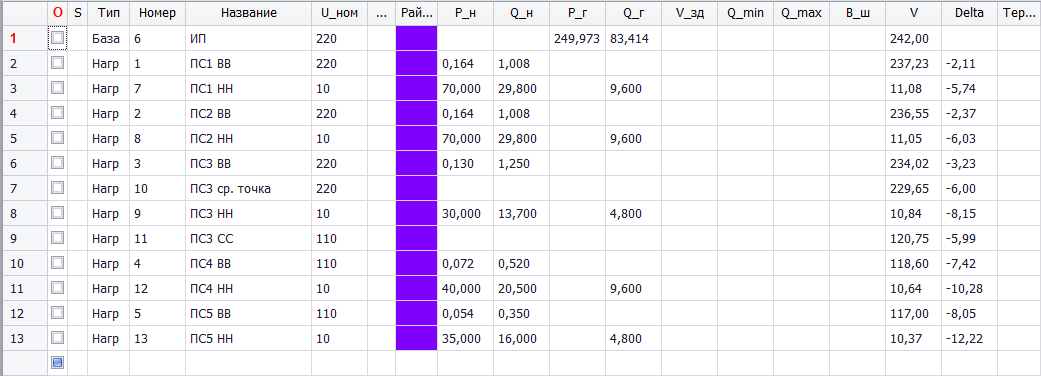
\includegraphics[width=1\textwidth]{inc/img/режим_нб_узлы}
	\caption{Исходные данные по узлам в режиме НБ и П/АВ и результаты расчёта режима НБ во вкладке «Узлы» без регулирования напряжений}
	\label{fig:узлы_нб}
\end{figure}

\begin{figure}[H]
	\centering
	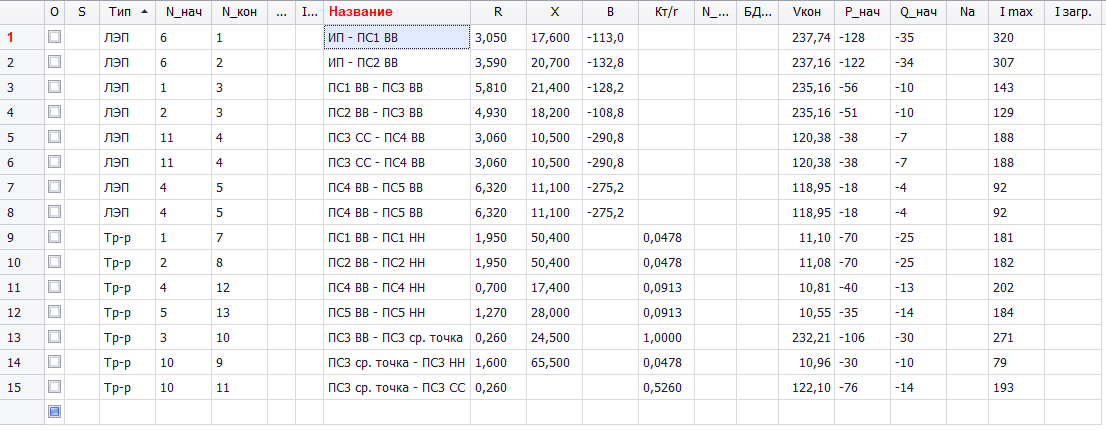
\includegraphics[width=1\textwidth]{inc/img/режим_нб_ветви}
	\caption{Исходные данные по узлам в режиме НБ и П/АВ и результаты расчета режима НБ во вкладке «Ветви» без регулирования напряжений}
	\label{fig:ветви_нб}
\end{figure}

Параметры регулировочных устройств приведены на рис \ref{fig:анцапфы}.

\begin{figure}[H]
	\centering
	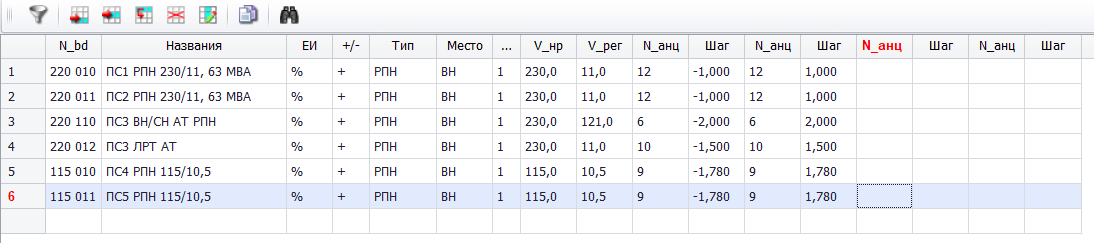
\includegraphics[width=1\textwidth]{inc/img/режим_нб_рпн}
	\caption{Параметры регулировочный устройств}
	\label{fig:анцапфы}
\end{figure}

Результаты регулировки напряжений в режиме НБ приведены на рис. \ref{fig:узлы_нб_отрег}, \ref{fig:ветви_нб_отрег}.

\begin{figure}[H]
	\centering
	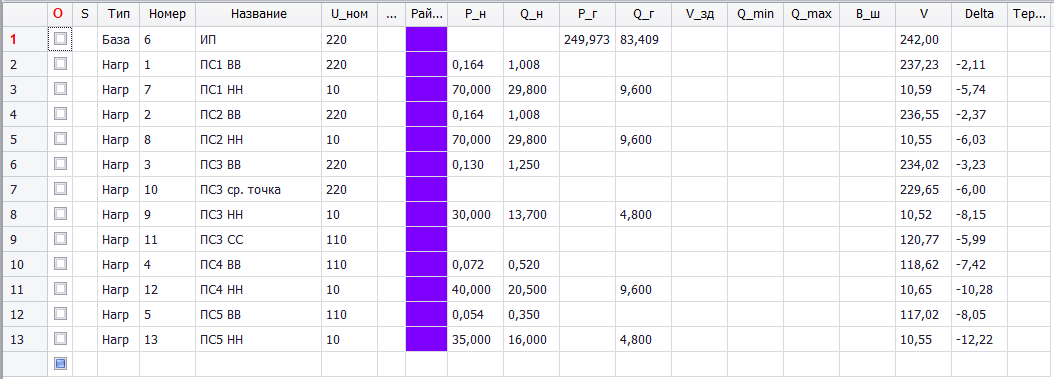
\includegraphics[width=1\textwidth]{inc/img/режим_нб_узлы_отрег}
	\caption{Результаты расчёта режима НБ после регулирования напряжения во вкладке «Узлы»}
	\label{fig:узлы_нб_отрег}
\end{figure}

\begin{figure}[H]
	\centering
	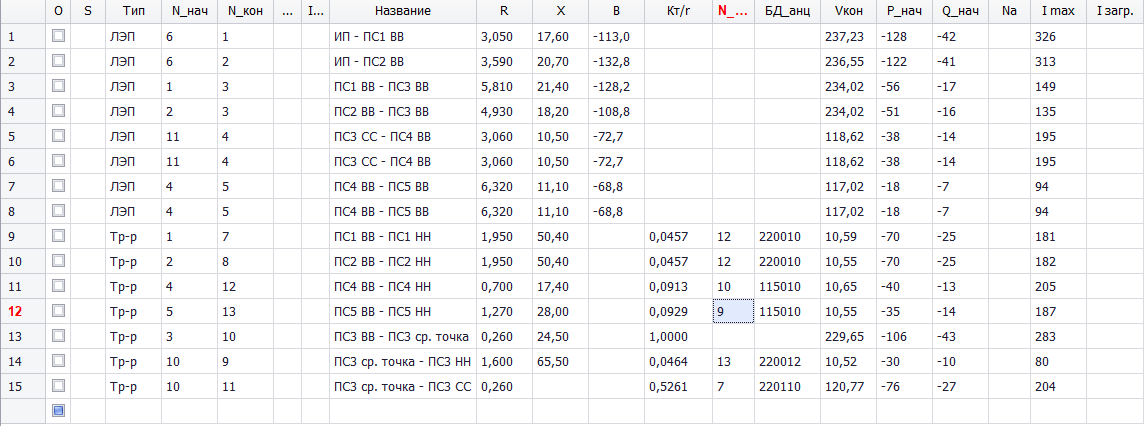
\includegraphics[width=1\textwidth]{inc/img/режим_нб_ветви_отрег}
	\caption{Результаты расчёта режима НБ после регулирования напряжения во вкладке «Ветви»}
	\label{fig:ветви_нб_отрег}
\end{figure}

\section{Моделирование и расчет режима наименьший нагрузок}

Параметры узлов для режима НМ приведены на рис. \ref{fig:режим_нм_узлы}, параметры ветвей для режима НМ приведены на рис. \ref{fig:режим_нм_ветви}.

\begin{figure}[H]
	\centering
	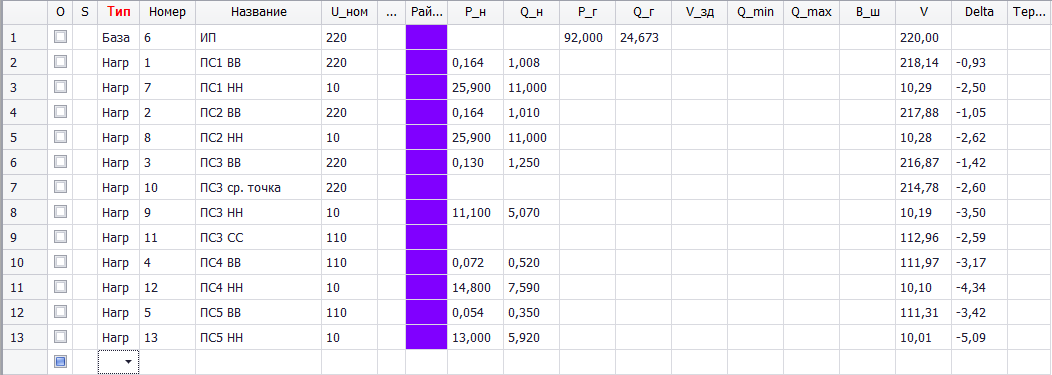
\includegraphics[width=1\textwidth]{inc/img/режим_нм_узлы}
	\caption{Исходные данные по узлам и результаты расчёта режима НМ во вкладке «Узлы» без регулирования напряжений}
	\label{fig:режим_нм_узлы}
\end{figure}

\begin{figure}[H]
	\centering
	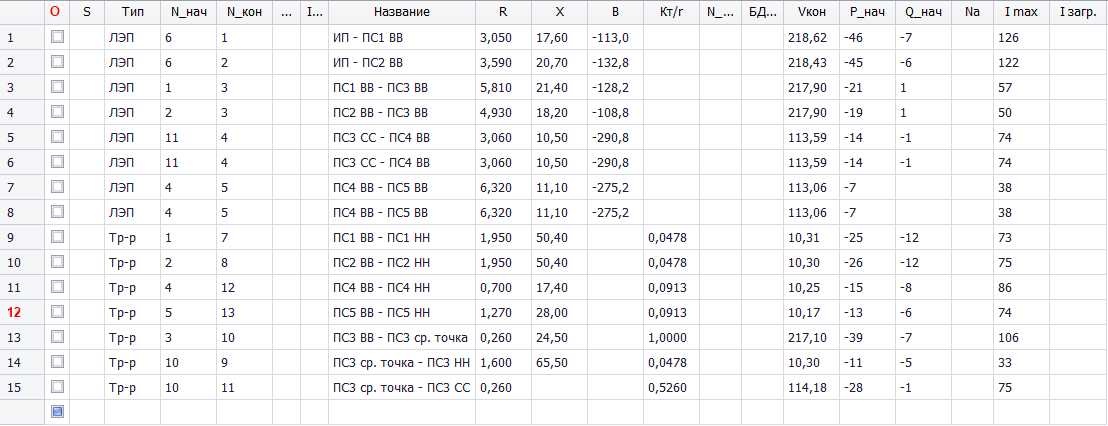
\includegraphics[width=0.8\textwidth]{inc/img/режим_нм_ветви}
	\caption{Исходные данные по ветвям и результаты расчета режима НМ во вкладке «Ветви» без регулирования напряжений}
	\label{fig:режим_нм_ветви}
\end{figure}

Результаты регулировки напряжений в режиме НМ приведены на рис. \ref{fig:режим_нм_узлы_отрег}, \ref{fig:режим_нм_ветви_отрег}.

\begin{figure}[H]
	\centering
	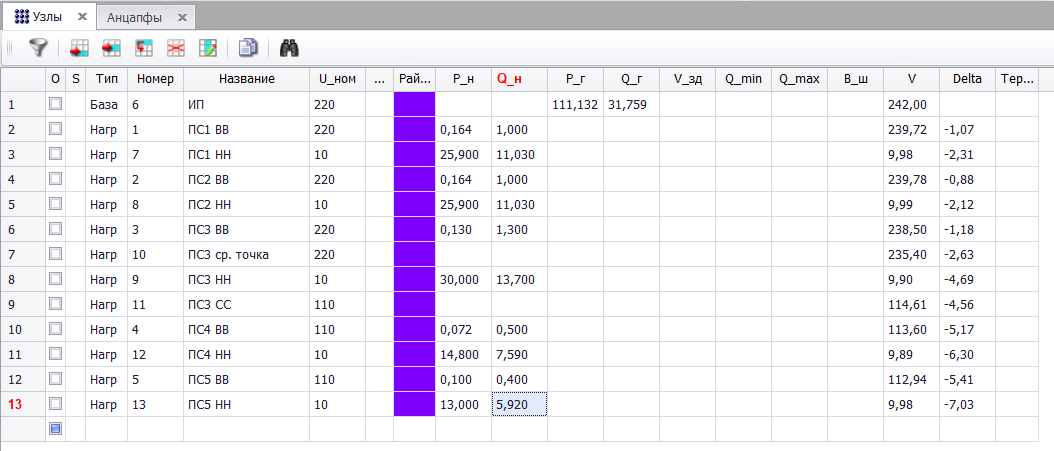
\includegraphics[width=1\textwidth]{inc/img/режим_нм_узлы_отрег}
	\caption{Результаты расчёта режима НМ во вкладке «Узлы» после регулирования напряжений}
	\label{fig:режим_нм_узлы_отрег}
\end{figure}

\begin{figure}[H]
	\centering
	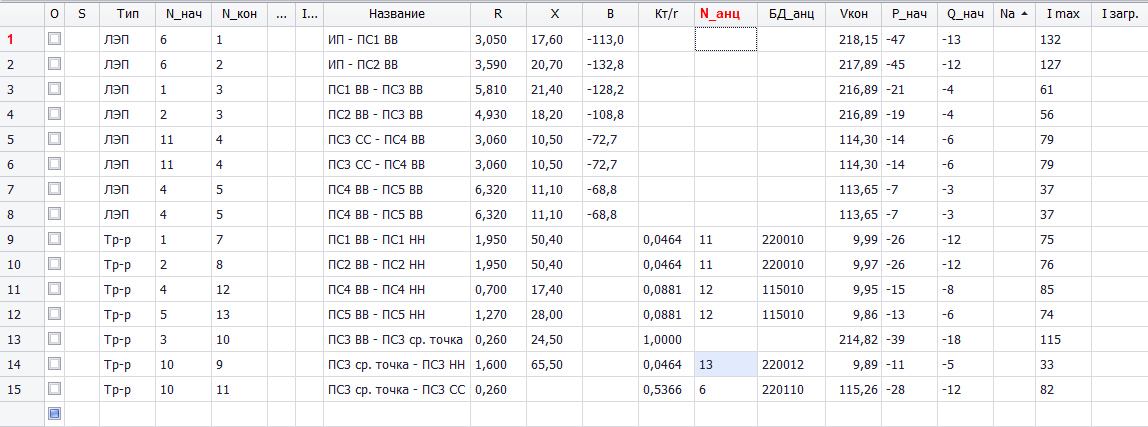
\includegraphics[width=0.8\textwidth]{inc/img/режим_нм_ветви_отрег}
	\caption{Результаты расчёта режима НМ во вкладке «Ветви» после регулирования напряжений}
	\label{fig:режим_нм_ветви_отрег}
\end{figure}

\section{Моделирование и расчёт послеаварийных режимов}

\subsection{Моделирование и расчет послеаварийного режима в сети 220 кВ}

Рассматривается послеаварийный режим в сети 220 кВ, при котором происходит отключение наиболее загруженного головного участка К-1.

Параметры узлов для П/АВ режима в кольцевой сети 220 кВ приведены на рис. \ref{fig:п/ав_в_сети_220_кв_узлы}, параметры ветвей для П/АВ режима в сети 220 кВ приведены на рис. \ref{fig:п/ав_в_сети_220_кв_ветви}.

\begin{figure}[H]
	\centering
	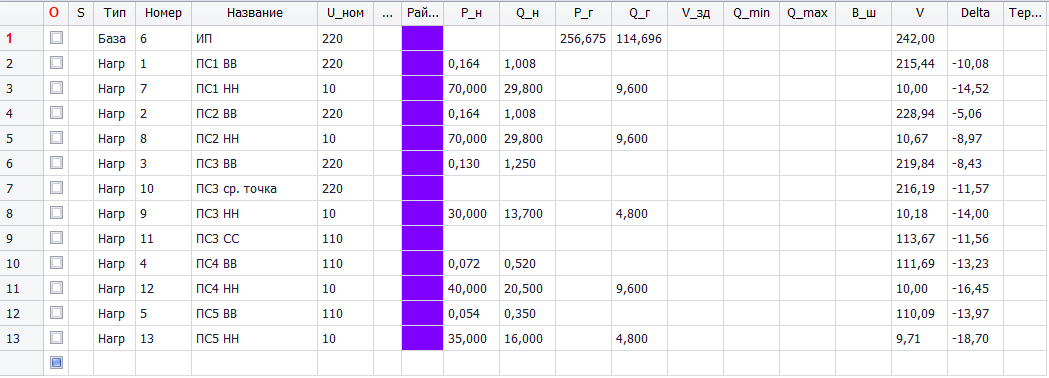
\includegraphics[width=1\textwidth]{inc/img/п_ав_220_кв_узлы}
	\caption{Результаты расчета П/АВ режима в сети 220 кВ при отключении линии К1 во вкладке «Узлы» без регулирования напряжений}
	\label{fig:п/ав_в_сети_220_кв_узлы}
\end{figure}

\begin{figure}[H]
	\centering
	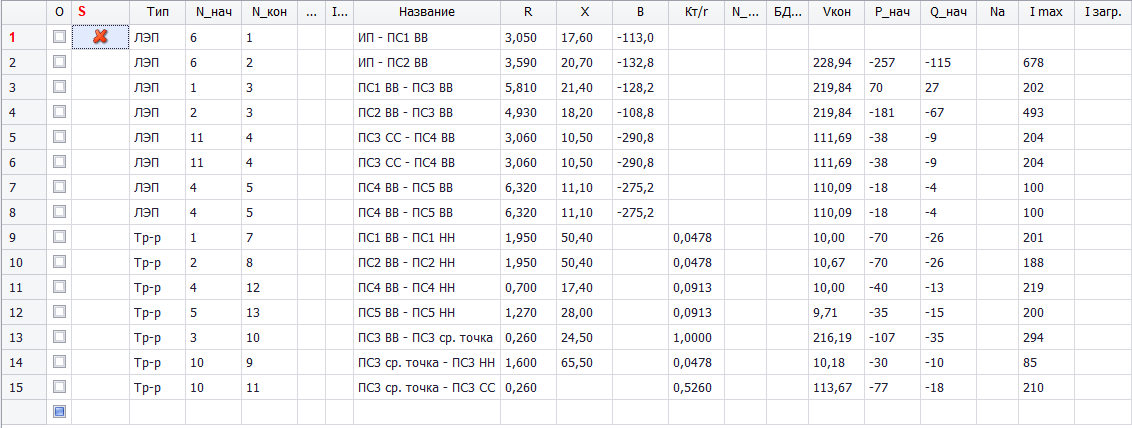
\includegraphics[width=1\textwidth]{inc/img/п_ав_220_кв_ветви}
	\caption{Результаты расчета П/АВ режима в сети 220 кВ при отключении линии К1 во вкладке «Ветви» без регулирования напряжений}
	\label{fig:п/ав_в_сети_220_кв_ветви}
\end{figure}

Результаты регулировки напряжений в режиме П/АВ в сети 220 кВ приведены на рис. \ref{fig:п/ав_в_сети_220_кв_узлы_отрег}, рис. \ref{fig:п/ав_в_сети_220_кв_ветви_отрег}.

\begin{figure}[H]
	\centering
	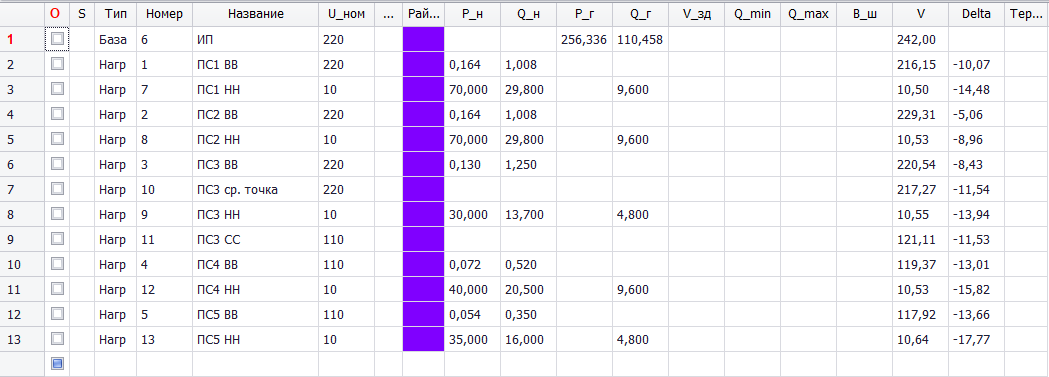
\includegraphics[width=1\textwidth]{inc/img/п_ав_220_кв_узлы_отрег}
	\caption{Регулирование напряжения на шинах НН и СН в П/АВ режиме в сети 220 кВ во вкладке «Узлы»}
	\label{fig:п/ав_в_сети_220_кв_узлы_отрег}
\end{figure}

\begin{figure}[H]
	\centering
	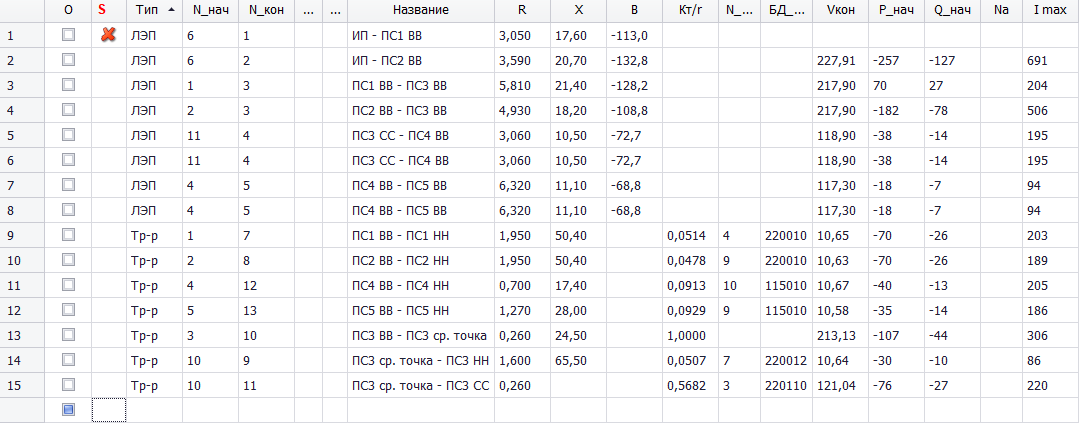
\includegraphics[width=1\textwidth]{inc/img/п_ав_220_кв_ветви_отрег}
	\caption{Регулирование напряжения на шинах НН и СН в П/АВ режиме в сети 220 кВ во вкладке «Ветви»}
	\label{fig:п/ав_в_сети_220_кв_ветви_отрег}
\end{figure}

\subsection{Моделирование и расчет послеаварийного режима в сети 110 кВ}

Рассматривается послеаварийный режим в сети 110 кВ, при котором происходит отключение одной цепи двухцепной линии 3-4.

Параметры узлов для П/АВ режима в сети 110 кВ приведены на рис. \ref{fig:п/ав_в_сети_110_кв_узлы}, параметры ветвей для П/АВ режима в сети 110 кВ приведены на рис. \ref{fig:п/ав_в_сети_110_кв_ветви}.

\begin{figure}[H]
	\centering
	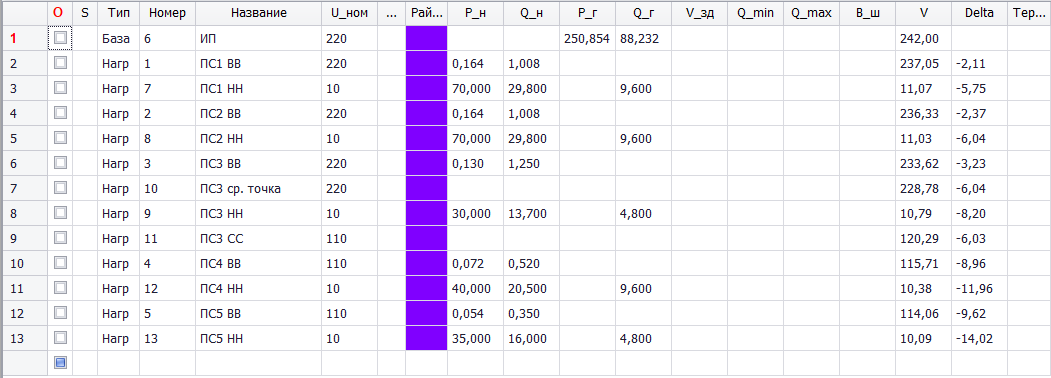
\includegraphics[width=1\textwidth]{inc/img/п_ав_110_кв_узлы}
	\caption{Результаты расчета после отключения наиболее нагруженного головного участка 34 для моделирования П/АВ режима в сети 110 кВ во вкладке «Узлы» без регулирования напряжений}
	\label{fig:п/ав_в_сети_110_кв_узлы}
\end{figure}

\begin{figure}[H]
	\centering
	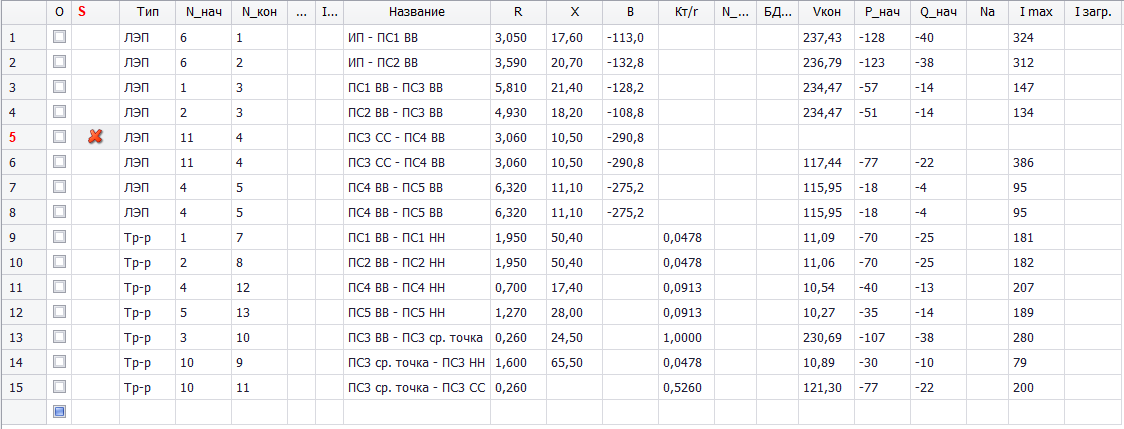
\includegraphics[width=1\textwidth]{inc/img/п_ав_110_кв_ветви}
	\caption{Результаты расчета после отключения наиболее нагруженного головного участка 34 для моделирования П/АВ режима в сети 110 кВ во вкладке «Ветви» без регулирования напряжений}
	\label{fig:п/ав_в_сети_110_кв_ветви}
\end{figure}

Результаты регулировки напряжений в П/АВ режиме в сети 110 кВ приведены на рис. \ref{fig:п/ав_в_сети_110_кв_узлы_отрег}, рис. \ref{fig:п/ав_в_сети_110_кв_ветви_отрег}.

\begin{figure}[H]
	\centering
	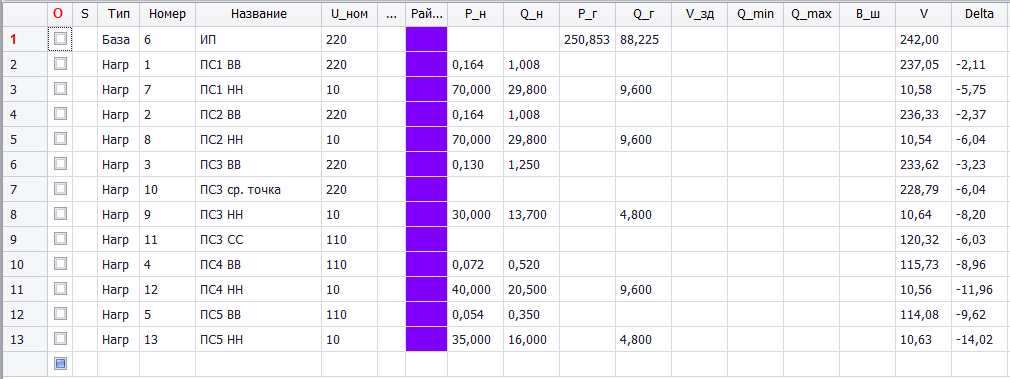
\includegraphics[width=1\textwidth]{inc/img/п_ав_110_кв_узлы_отрег}
	\caption{Результаты регулирования напряжения на шинах НН и СН в П/АВ режиме в сети 110 кВ при отключении наиболее нагруженного головного участка 34 во вкладке «Узлы»}
	\label{fig:п/ав_в_сети_110_кв_узлы_отрег}
\end{figure}

\begin{figure}[H]
	\centering
	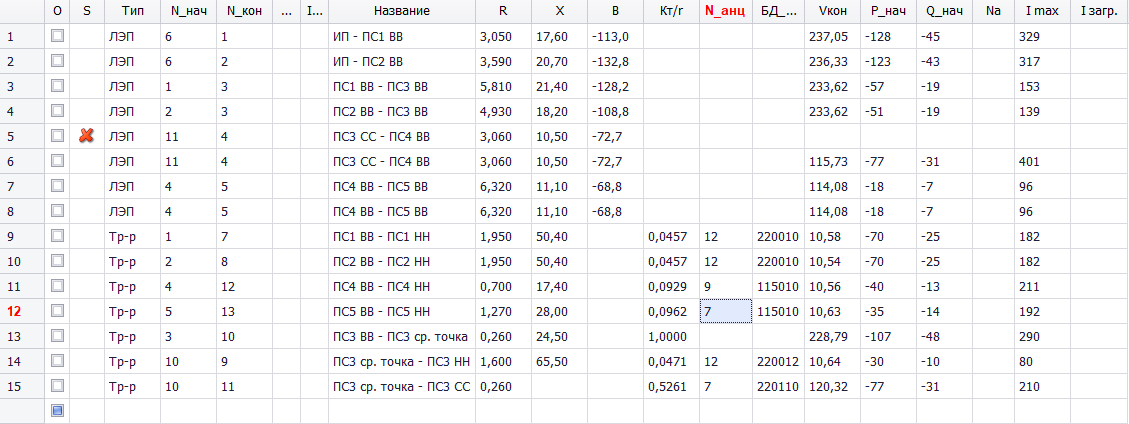
\includegraphics[width=1\textwidth]{inc/img/п_ав_110_кв_ветви_отрег}
	\caption{Результаты регулирования напряжения на шинах НН и СН в П/АВ режиме в сети 110 кВ при отключении наиболее нагруженного головного участка 34 во вкладке «Ветви»}
	\label{fig:п/ав_в_сети_110_кв_ветви_отрег}
\end{figure}

%\include{90-appendix1}

%\include{91-appendix2}

\end{document}

%%% Local Variables:
%%% mode: latex
%%% TeX-master: t
%%% End:
